%%____________________________________________________________________________||
\section{Interpretation in Simplified SUSY models}
\label{sec:susy}
To interpret the results of this search, simplified
%models~\cite{Alwall:2008ag,Alwall:2008va,Alves:2011wf} for the production of
supersymmetric particles are considered.  They use only a limited set of
sparticles in the production and decay and enable comprehensive studies of
individual SUSY event topologies. These studies can be performed in terms of
fundamental properties such as decay modes, production cross sections and
sparticle masses.

\subsection{Signal models}
\label{sec:susy_models}
Interpretations are presented for pair production of gluino, stop, sbottom and
scharm particles with several different possibilities for the decay chain. The
simplified models used in the analysis are summarised in
Tab.~\ref{tab:simplified-models}. Benchmark points are also listed, which will
be used throughout the section. Two benchmarks are provided, where relevant,
to cover the phenomenology of compressed and uncompressed spectra. All the
benchmarks are chosen to be right within the expected exclusion. \\
%A sensitivity study has been performed on these benchmark models, which is
%described in App.~\ref{app:sensitivity-benchmarks}. \\
Sketches of the production and decay in these models are shown in
Fig.~\ref{fig:simplified-models-feyn}. Systematic uncertainties on the signal
acceptance are detailed in Sec.~\ref{sec:sig-syst}.

All the models are generated using the FastSim package \cite{Abdullin:2011zz}.
FastSim Monte Carlo samples are corrected using FastSim-to-FullSim scale factor,
accounting for difference in b-tag efficiency. These scale factors are applied
on top of the FullSim scale factors applied for the other Monte Carlo samples.

\begin{table}[h!]
    \scriptsize
    \caption{A summary of the simplified models used in this analysis.}
    \label{tab:simplified-models}
    \centering
    \begin{tabular}{ lllllll }
        \hline \hline
        Model & Production & Decay & Previous limits & Figure & Benchmarks $(m_{\mathrm{Susy}},m_{\mathrm{LSP}})$ \\ 
        \hline \hline
        T1bbbb & \ppToGluGlu & \gluToBBNo & $m_{\mathrm{Gluino}}>\sim 1850 \,\mathrm{GeV}$ (ICHEP) & \ref{fig:T1bbbb_feyn} & \parbox[t]{5cm}{Compressed: (1300,1100)\\Uncompressed: (1900,100)} \\
        \hline
        T2tt   & \ppToStopStop & \stopToTNo & $m_{\mathrm{\mathrm{Stop}}}>\sim 925 \,\mathrm{GeV}$ (ICHEP) & \ref{fig:T2tt_feyn} & \parbox[t]{5cm}{Compressed: (450,200)\\Uncompressed: (1000,50)\\$W$ corridor: (250,150)} \\
        \hline
        T2cc   & \ppToStopStop & \stopToCNo & $m_{\mathrm{\mathrm{Stop}}}>\sim 350 \,\mathrm{GeV}$ (2015)& \ref{fig:T2cc_feyn} & Compressed: (500,480) \\
        \hline
        T2bb   & \ppToSbotSbot & \sbottomToB & $m_{\mathrm{\mathrm{Sbottom}}}>\sim 980 \,\mathrm{GeV}$ (ICHEP)& \ref{fig:T2bb_feyn} & \parbox[t]{5cm}{Compressed: (550,450)\\Uncompressed: (1000,100)} \\
        \hline \hline
    \end{tabular}
\end{table}

\begin{figure}[h!]
    \begin{center}
        \subfigure[T1bbbb]{
            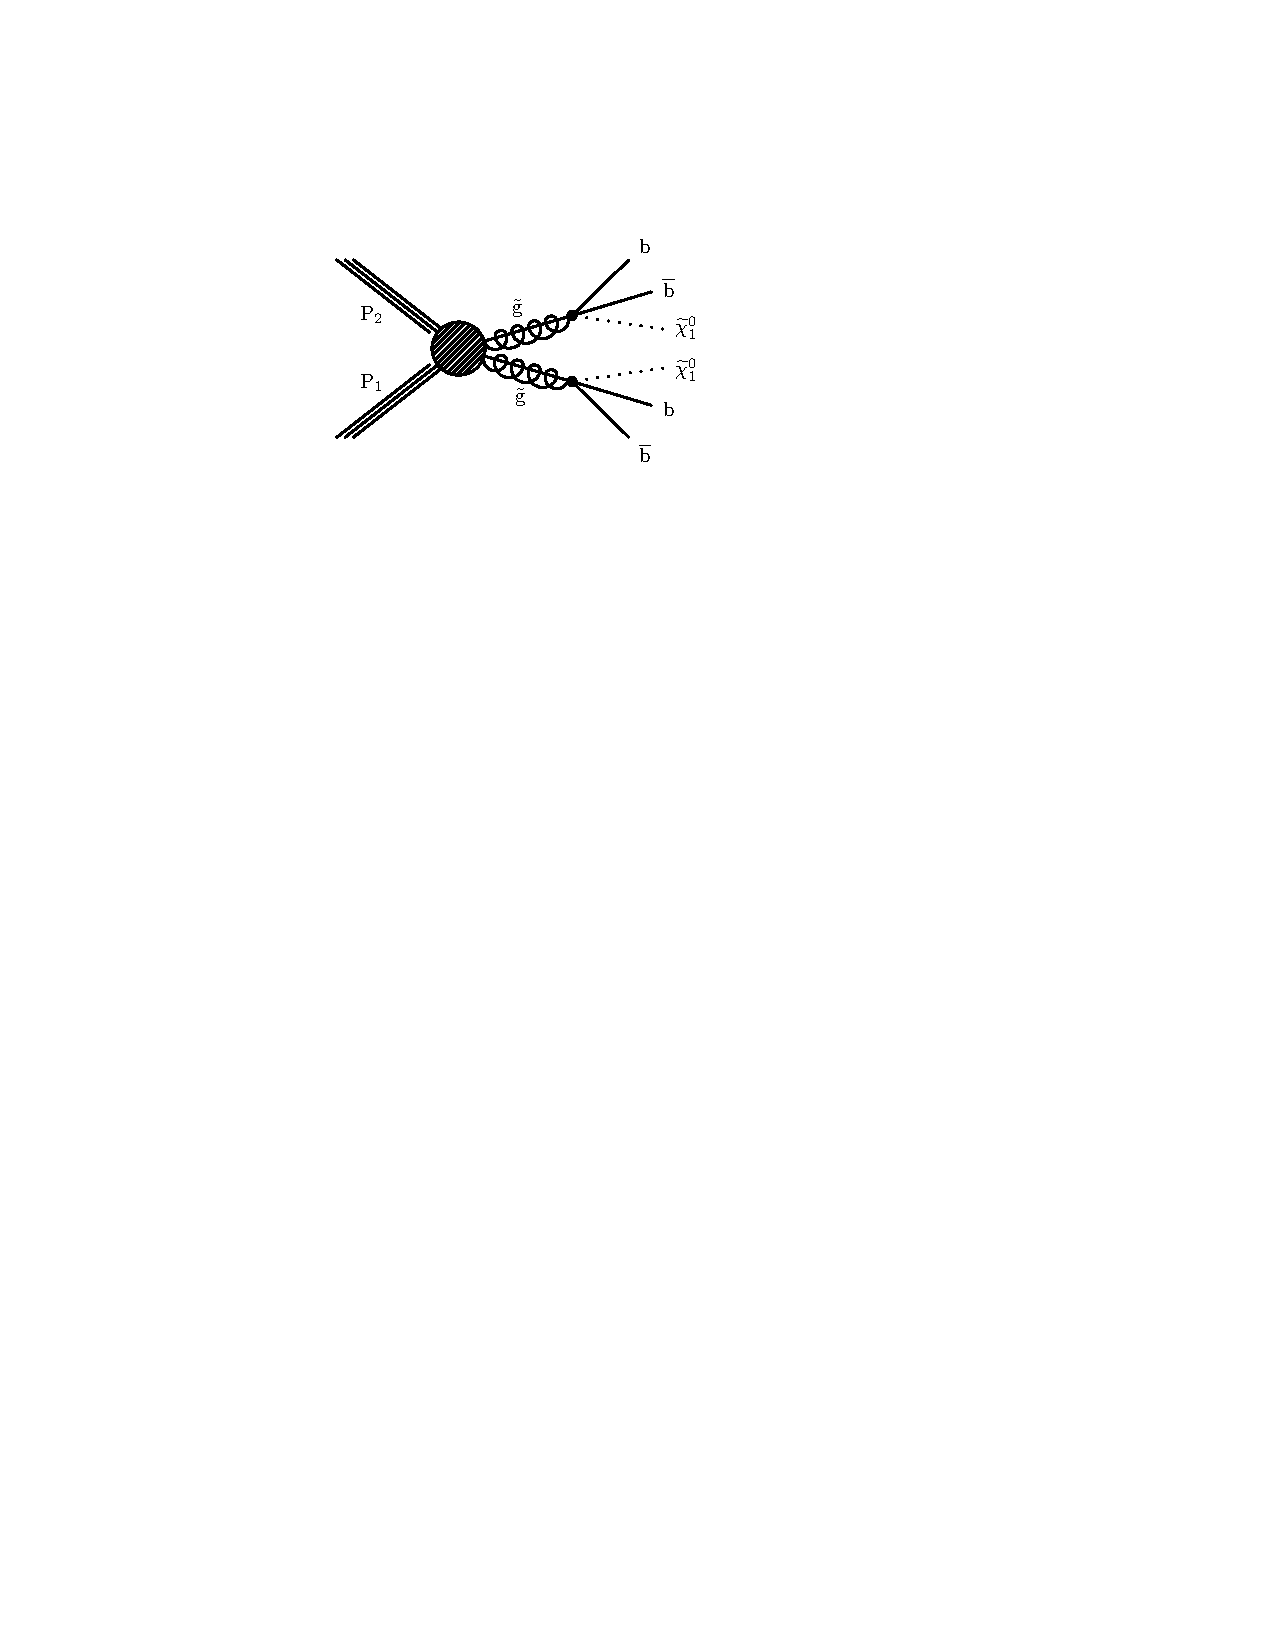
\includegraphics[width=0.35\textwidth]{figures/susyResults/T1bbbb_feyn}
            \label{fig:T1bbbb_feyn}
            } ~~
        \subfigure[T2tt]{
            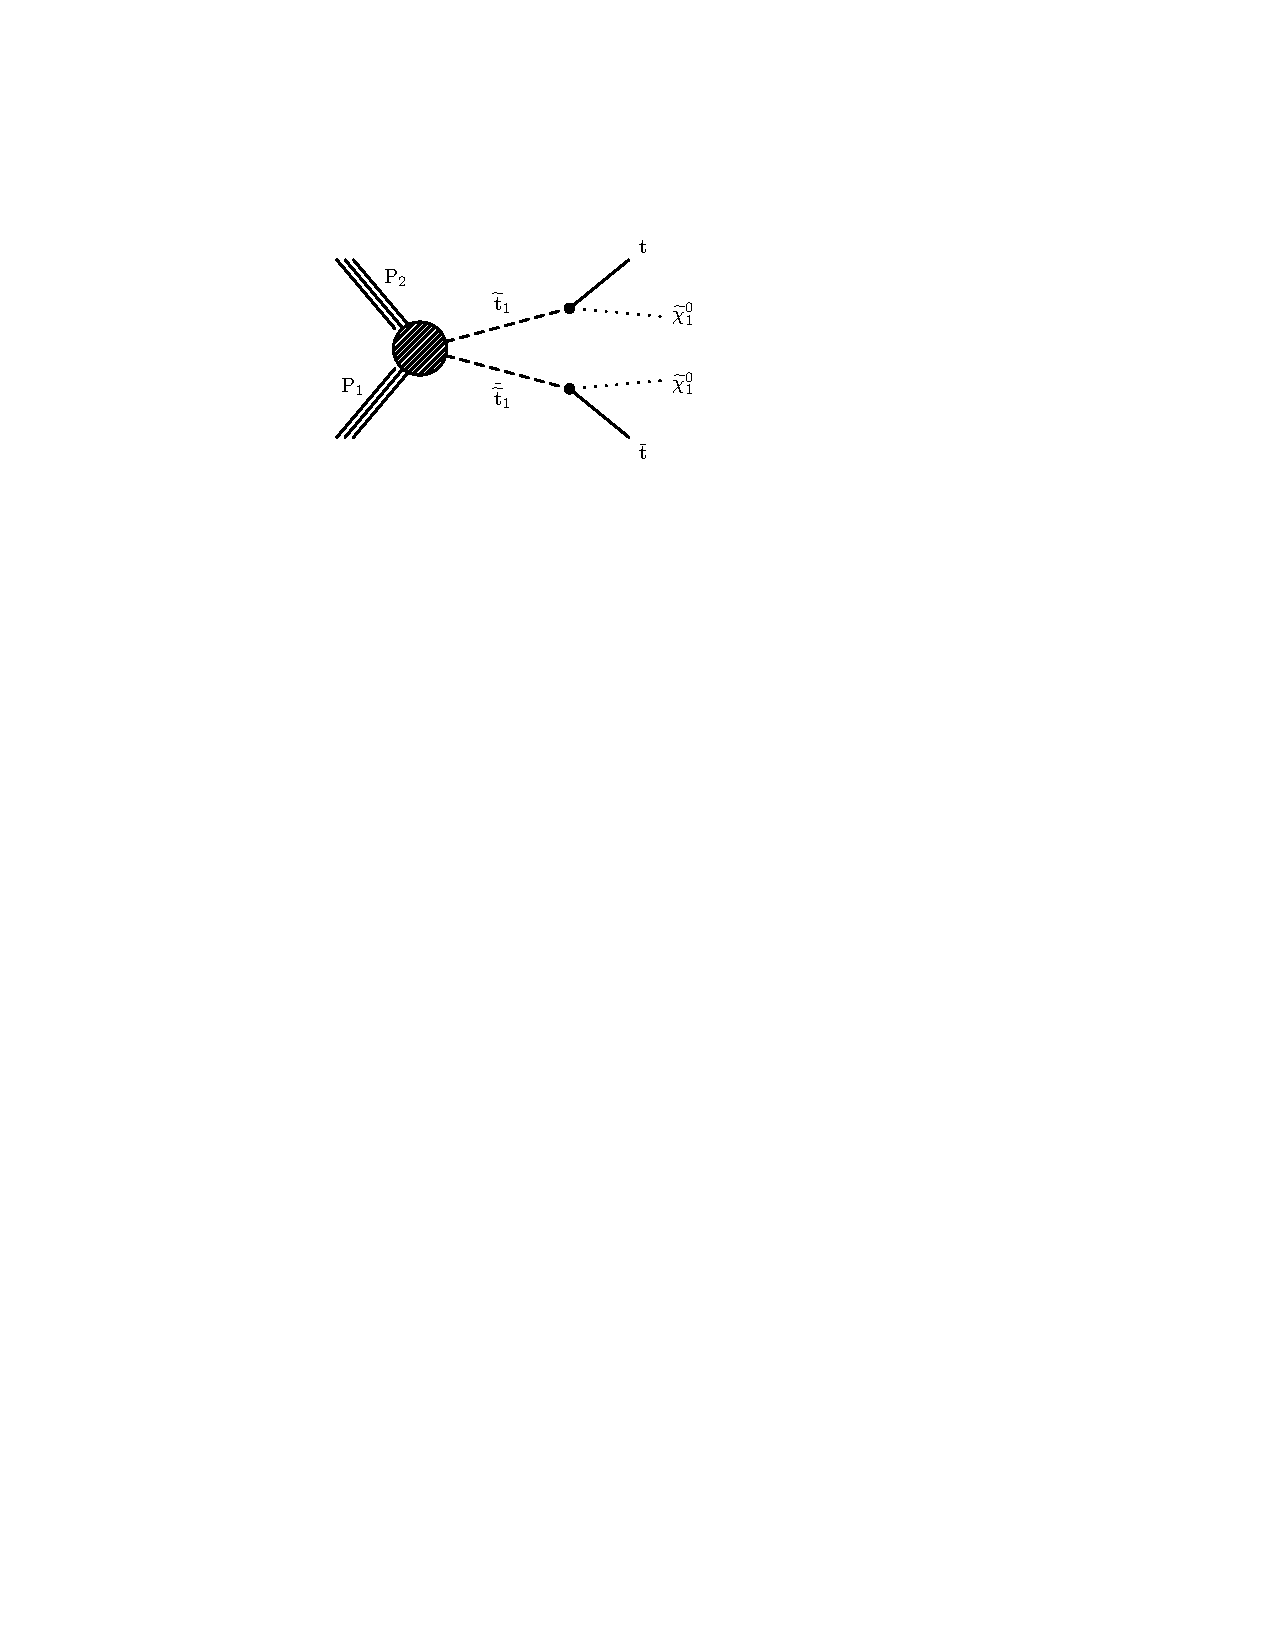
\includegraphics[width=0.35\textwidth]{figures/susyResults/T2tt_feyn}
            \label{fig:T2tt_feyn}
            } \\
        \subfigure[T2bb]{
            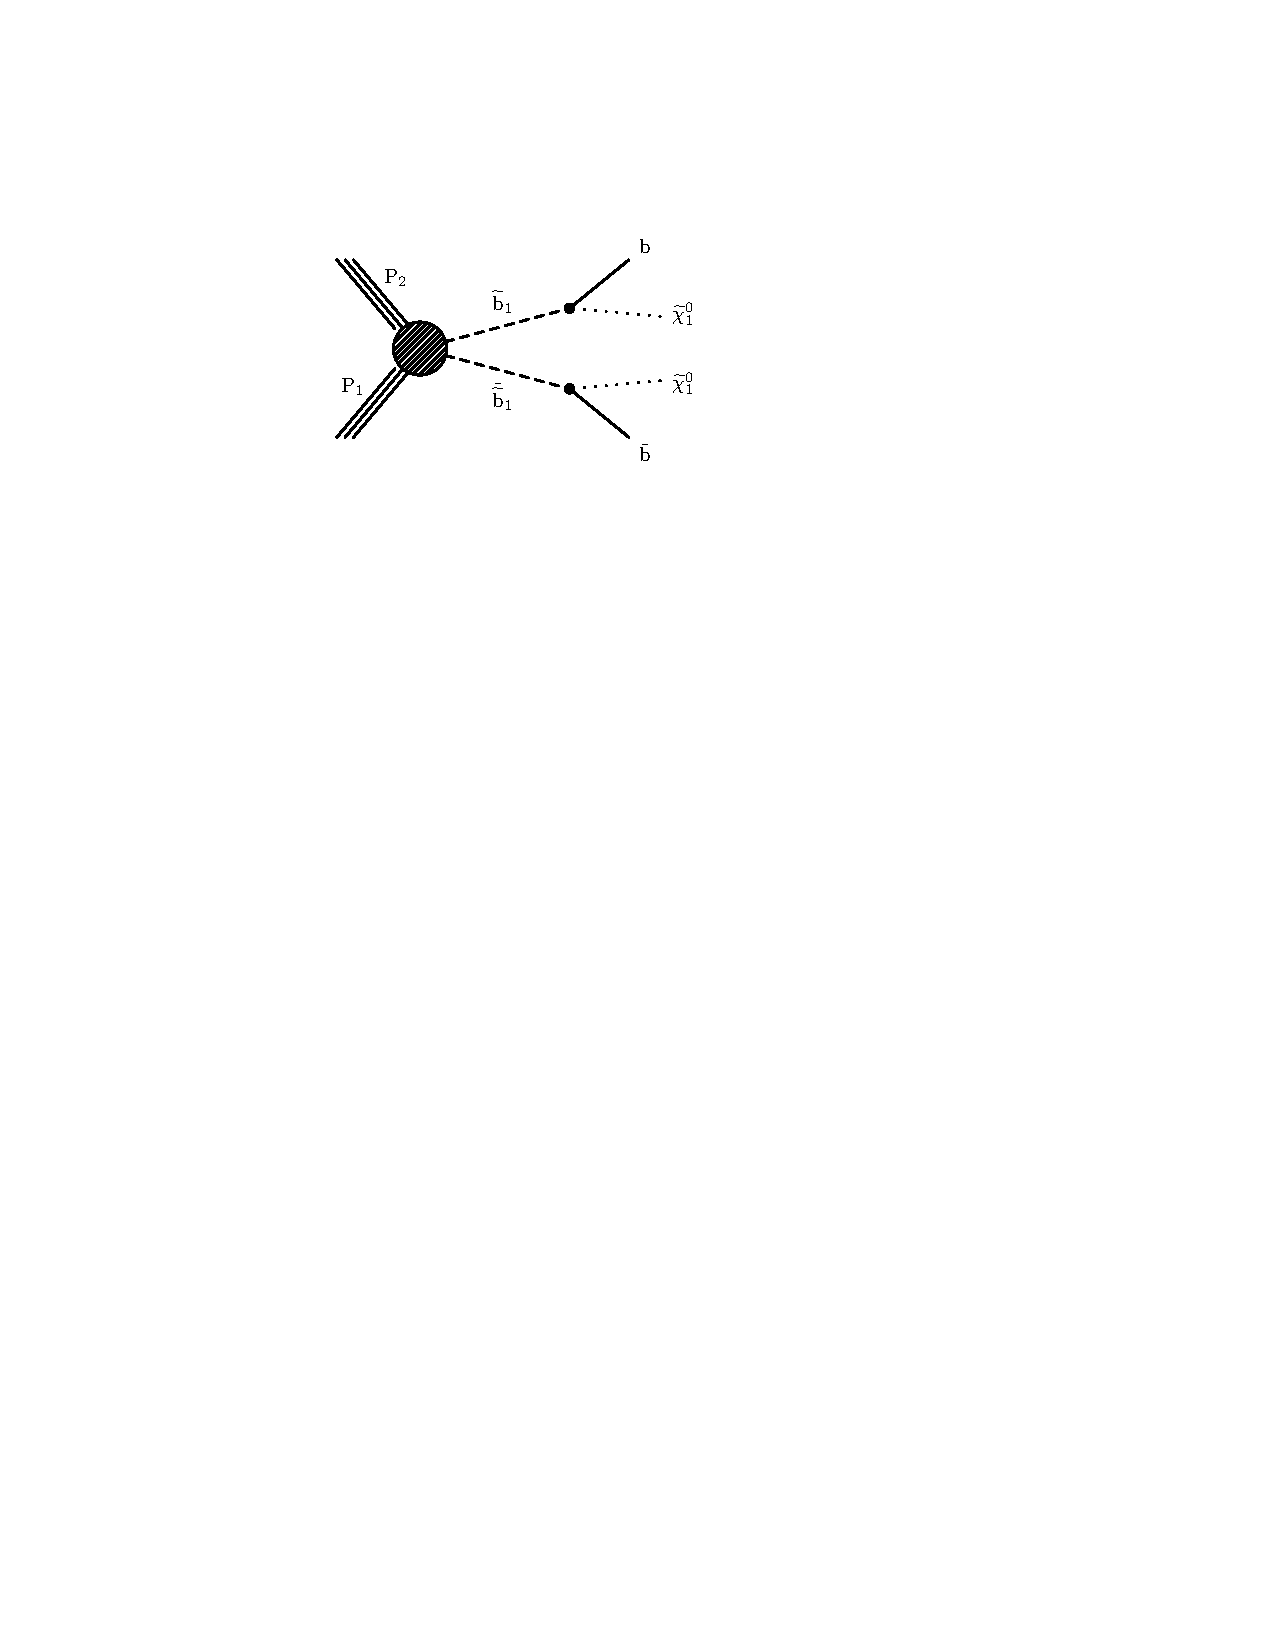
\includegraphics[width=0.35\textwidth]{figures/susyResults/T2bb_feyn}
            \label{fig:T2bb_feyn}
            }
        \subfigure[T2cc]{
            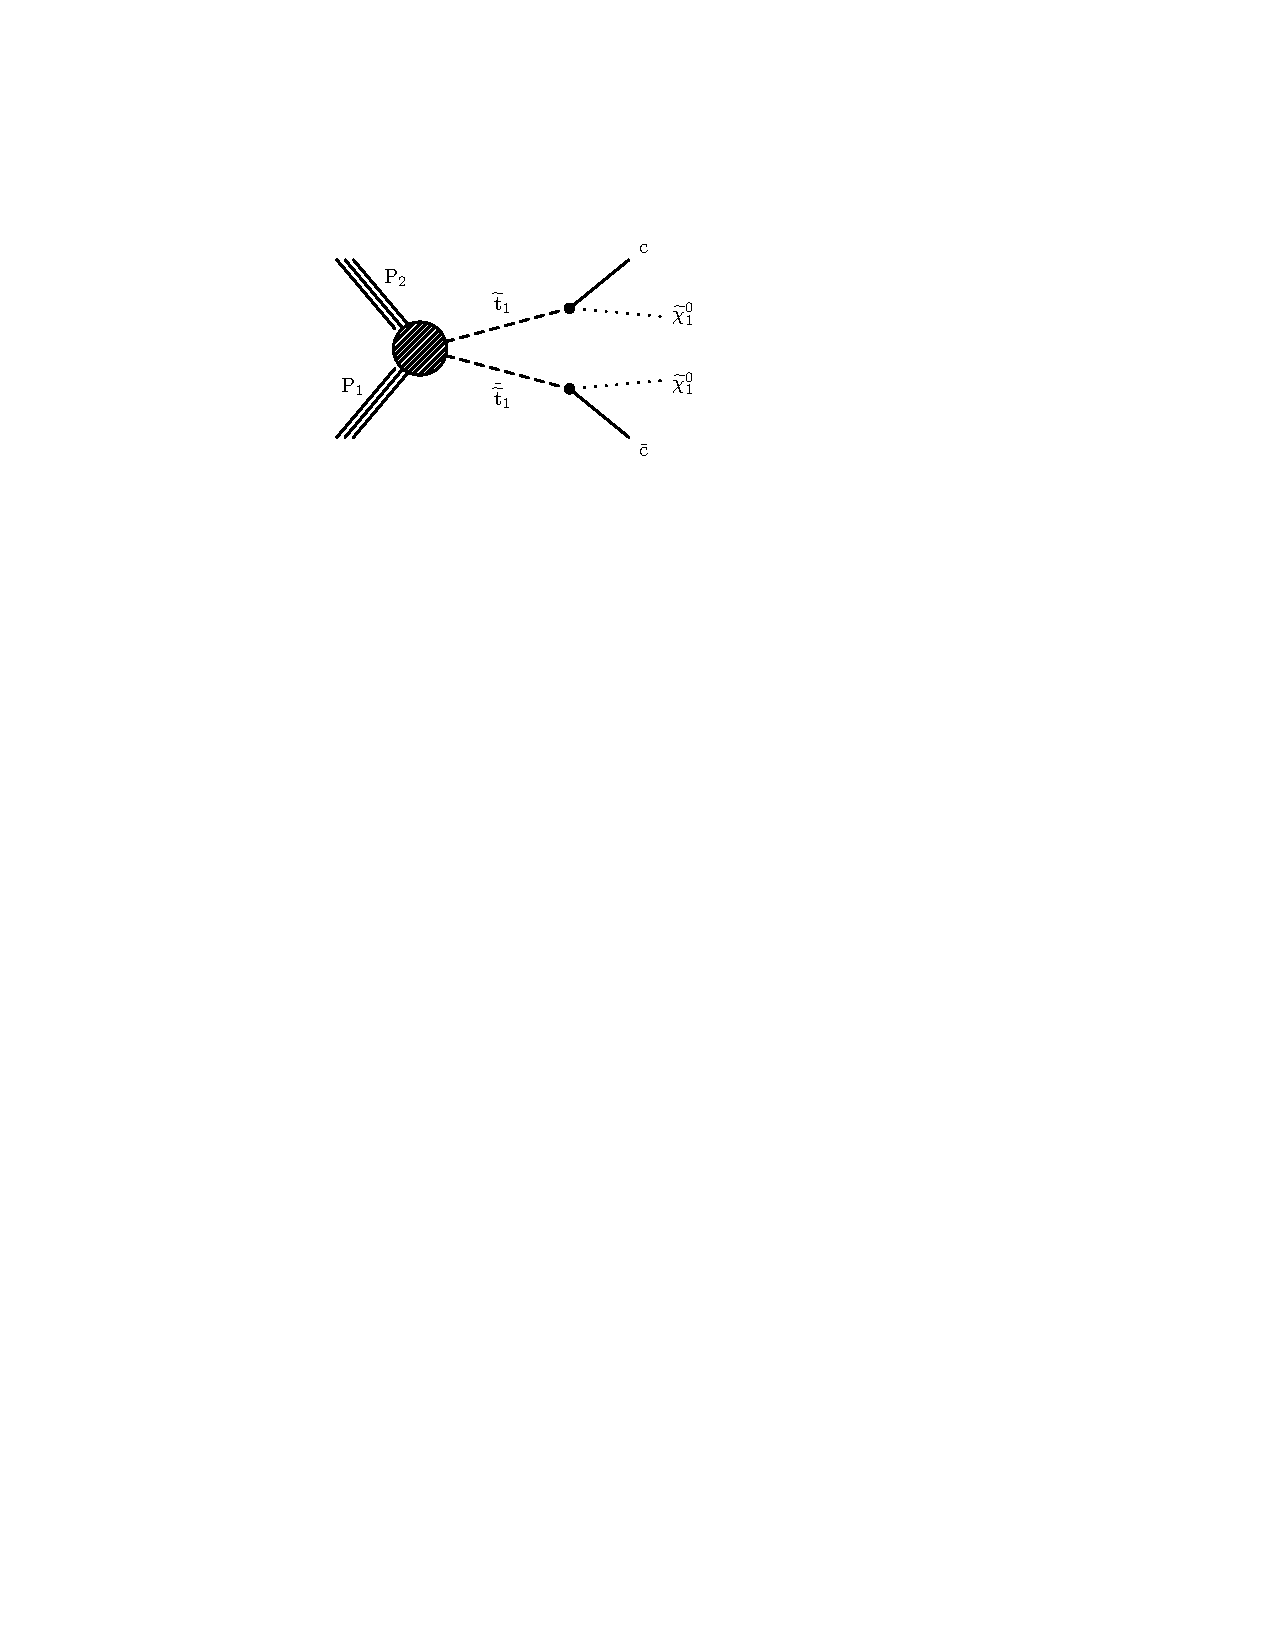
\includegraphics[width=0.35\textwidth]{figures/susyResults/T2cc_feyn}
            \label{fig:T2cc_feyn}
            } ~~
        \caption{Graphical representation of the production and decay of
            supersymmetric particles in models with the production of: (a)
            gluinos (with decoupled third generation squarks), (b) stops, (c)
            sbottoms and (d) scharms.}
        \label{fig:simplified-models-feyn}
    \end{center}
\end{figure}

\subsection{Signal acceptance}
\label{sec:sig-accept-contam}
In Tab. \ref{tab:sig-eff} the signal efficiency for benchmark mass points for
all the models is summarised. The signal efficiency across the whole
($m_{\mathrm{Susy}},m_{\mathrm{LSP}}$) for the simplified models used in the
analysis is shown in Fig.~\ref{fig:T1bbbb_eff}-\ref{fig:T2cc_eff}.

\begin{table}[h!]
    \caption{Signal efficiency for compressed and uncompressed models used in
        the analysis.}
    \label{tab:sig-eff}
    \centering
    \begin{tabular}{ lllll }
        \hline \hline
        Model & $(m_{\mathrm{Susy}},m_{\mathrm{LSP}})$ & Efficiency (total) \\ 
        \hline
        \multirow{2}{*}{T1bbbb}
            & (1900,100)  & 25.0\% \\
            & (1300,1100) & 14.6\% \\
        \hline
        \multirow{2}{*}{T2tt}
            & (1000,50) & 24.0\% \\
            & (450,200) & 4.2\% \\
            & (250,150) & 0.27\% \\
        \hline
        T2cc
            & (500,480) & 20.5\% \\
        \hline
        \multirow{2}{*}{T2bb}
            & (1000,100) & 40.0\% \\
            & (550,450)  & 5.7\% \\
        \hline \hline
    \end{tabular}
\end{table}

%The level of signal contamination in the control regions is expected to be
%negligible for most of the models that are targeted by this search. The
%requirement of one muon or two muons in the \mj and \mmj respectively ensures
%that the control regions are depleted from signal events, in the case where the
%final state is all-hadronic. The only partial exception is the stop pair
%production followed by decay into top quarks, called T2tt. In this case, when
%top decays leptonically, a residual signal contamination may be found in the
%muon control regions. However, the kinematic selection applied to the control
%regions, like the absence of any \alt cut and the $m_{T}$ cut, helps to reduce
%the signal contamination. \\
%The metric that is chosen to study the signal contamination in the following is
%the double-ratio $(S_{SR}/B_{SR})/(S_{CR}/B_{CR})$, as the sensitivity of the
%control region ($S_{CR}/B_{CR}$) is expected to be small compared to the one in
%the signal region ($S_{SR}/B_{SR}$) by definition.
%
%Fig.~\ref{fig:contamination_T2tt} characterises the level of signal
%contamination for the T2tt ($m_{\mathrm{Stop}}=XXX$ GeV, $m_{\mathrm{LSP}}=YYY$ GeV)
%model, as a function of event category and \scalht bin. This benchmark point
%has $m_{\mathrm{Susy}}-m_{\mathrm{LSP}} \sim m_{\mathrm{top}}$, which is the
%scenario where the largest signal contamination is expected, since the
%kinematics is similar to the top quark production, which is more likely to
%satisfy the control region selection with respect to the signal region. \\
%Fig. ~\ref{fig:contamination_T2tt_yields_had} and
%~\ref{fig:contamination_T2tt_yields_had} show the expected signal yield counts
%in the signal region and \mj control region respectively, for the T2tt benchmark
%model. Fig.~\ref{fig:contamination_T2tt_relEff} shows the ratio of signal
%contamination to signal efficiency of the signal region, for the T2tt benchmark
%model. Fig.~\ref{fig:contamination_T2tt_doubleRatio} shows the ratio of
%sensitivity in the control region to the sensitivity in the signal region, for
%T2tt benchmark model. The sensitivity is defined as the ratio of signal to
%background expected counts.

%\begin{figure}[h!]
%    \begin{center}
%        \subfigure[Expected counts in the signal region]{
%            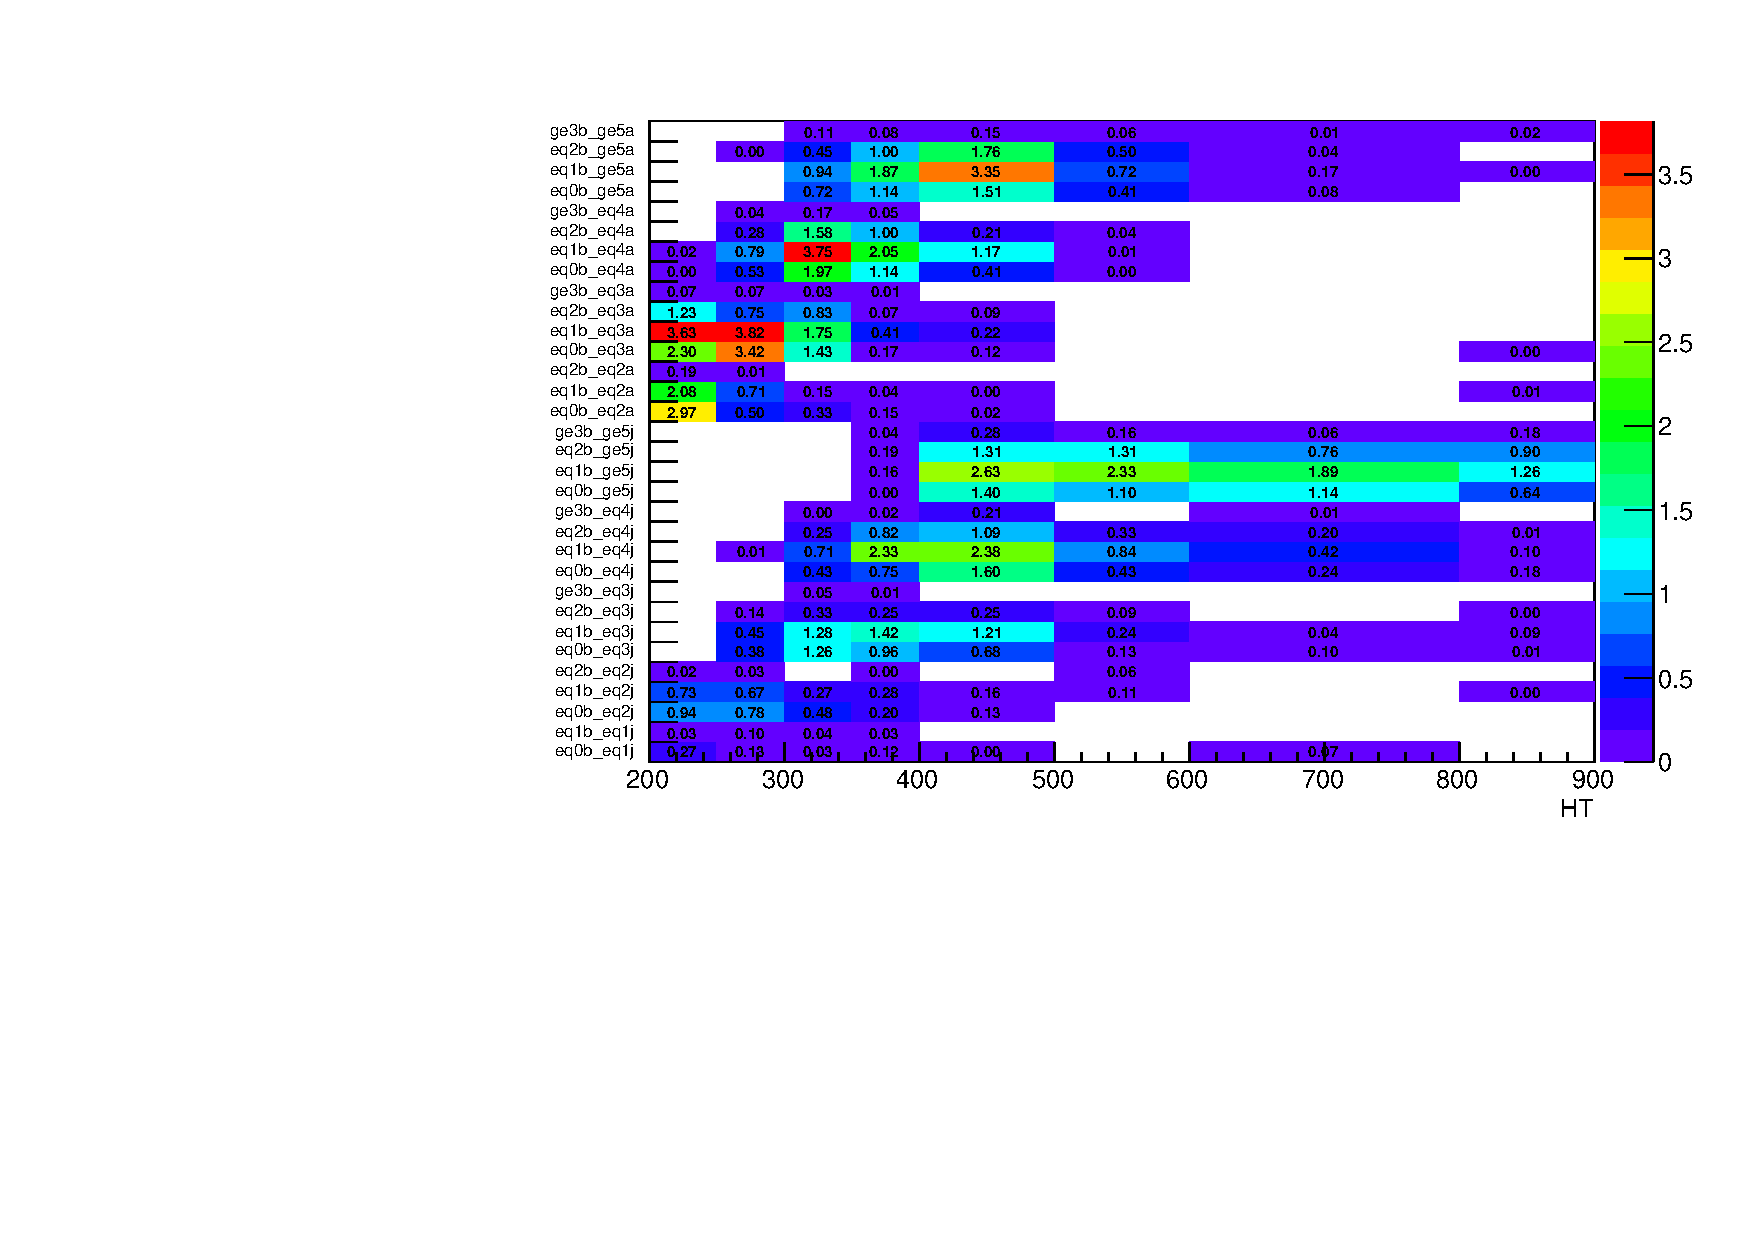
\includegraphics[width=0.5\textwidth]{figures/susyResults/sigYields_had_SMS-T2tt_mStop-250_mLSP-50_25ns}
%            \label{fig:contamination_T2tt_yields_had}
%        }
%        \subfigure[Expected counts in the \mj control region]{
%            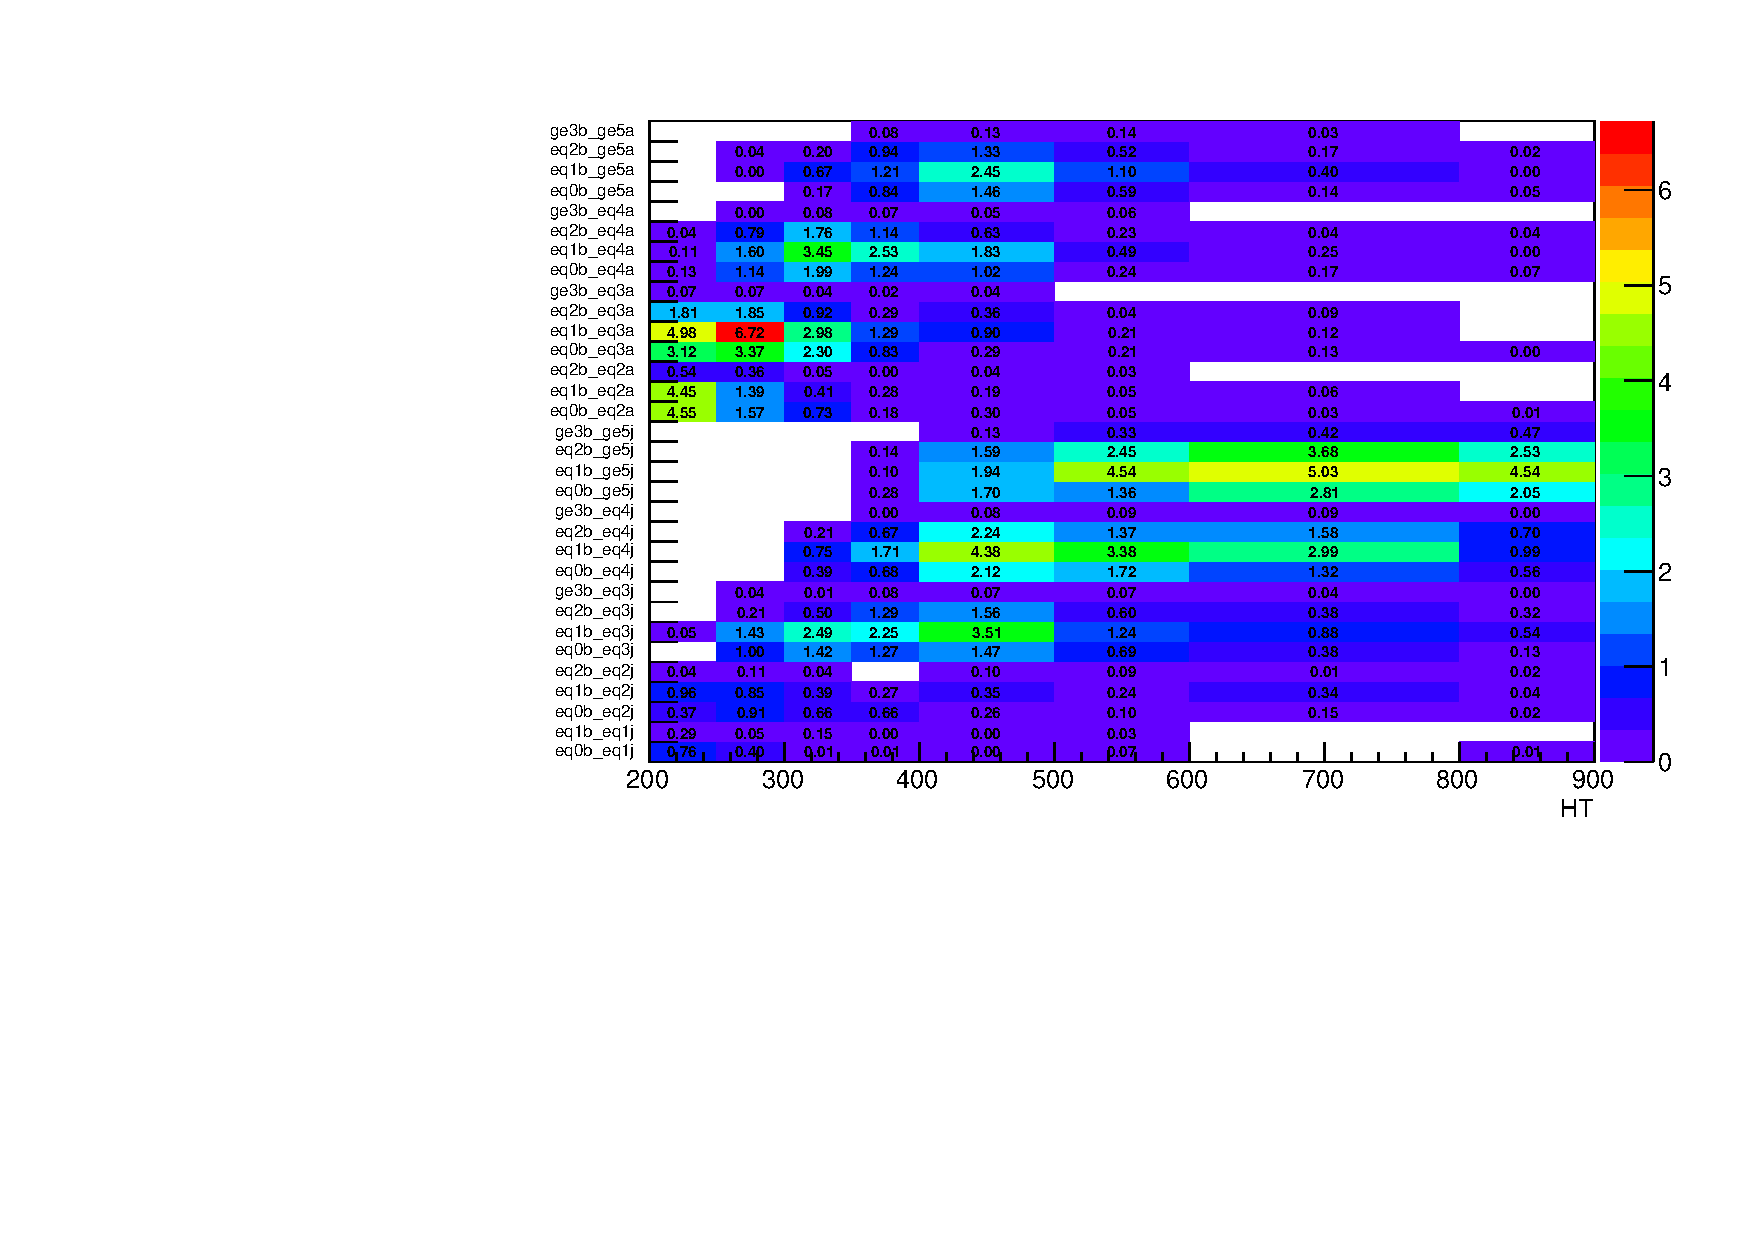
\includegraphics[width=0.5\textwidth]{figures/susyResults/sigYields_SingleMu_SMS-T2tt_mStop-250_mLSP-50_25ns}
%            \label{fig:contamination_T2tt_yields_mj}
%        } \\
%        \subfigure[Ratio of signal acceptance (\mj to signal region)]{
%            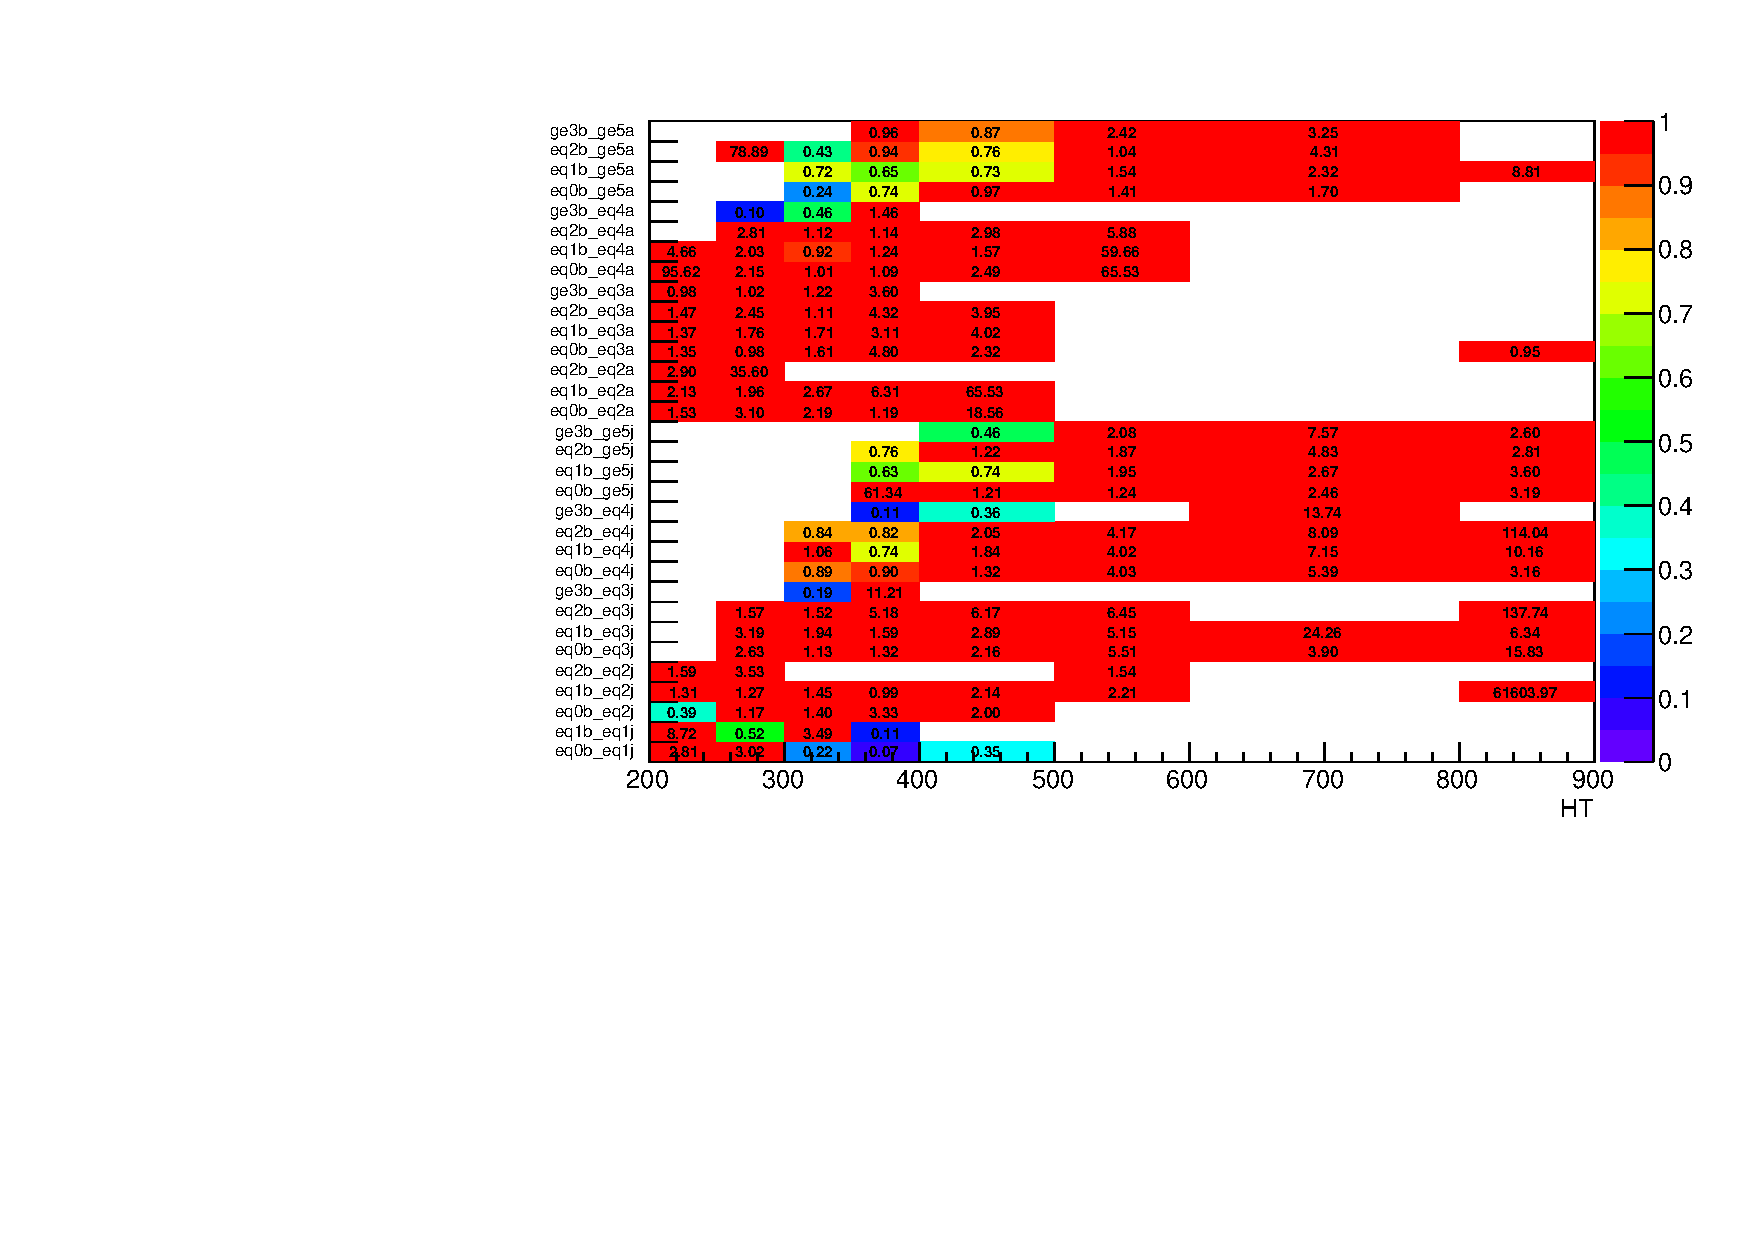
\includegraphics[width=0.5\textwidth]{figures/susyResults/relEff_SingleMu_SMS-T2tt_mStop-250_mLSP-50_25ns}
%            \label{fig:contamination_T2tt_relEff}
%        }
%        \subfigure[Ratio of S/B values (\mj to signal region)]{
%            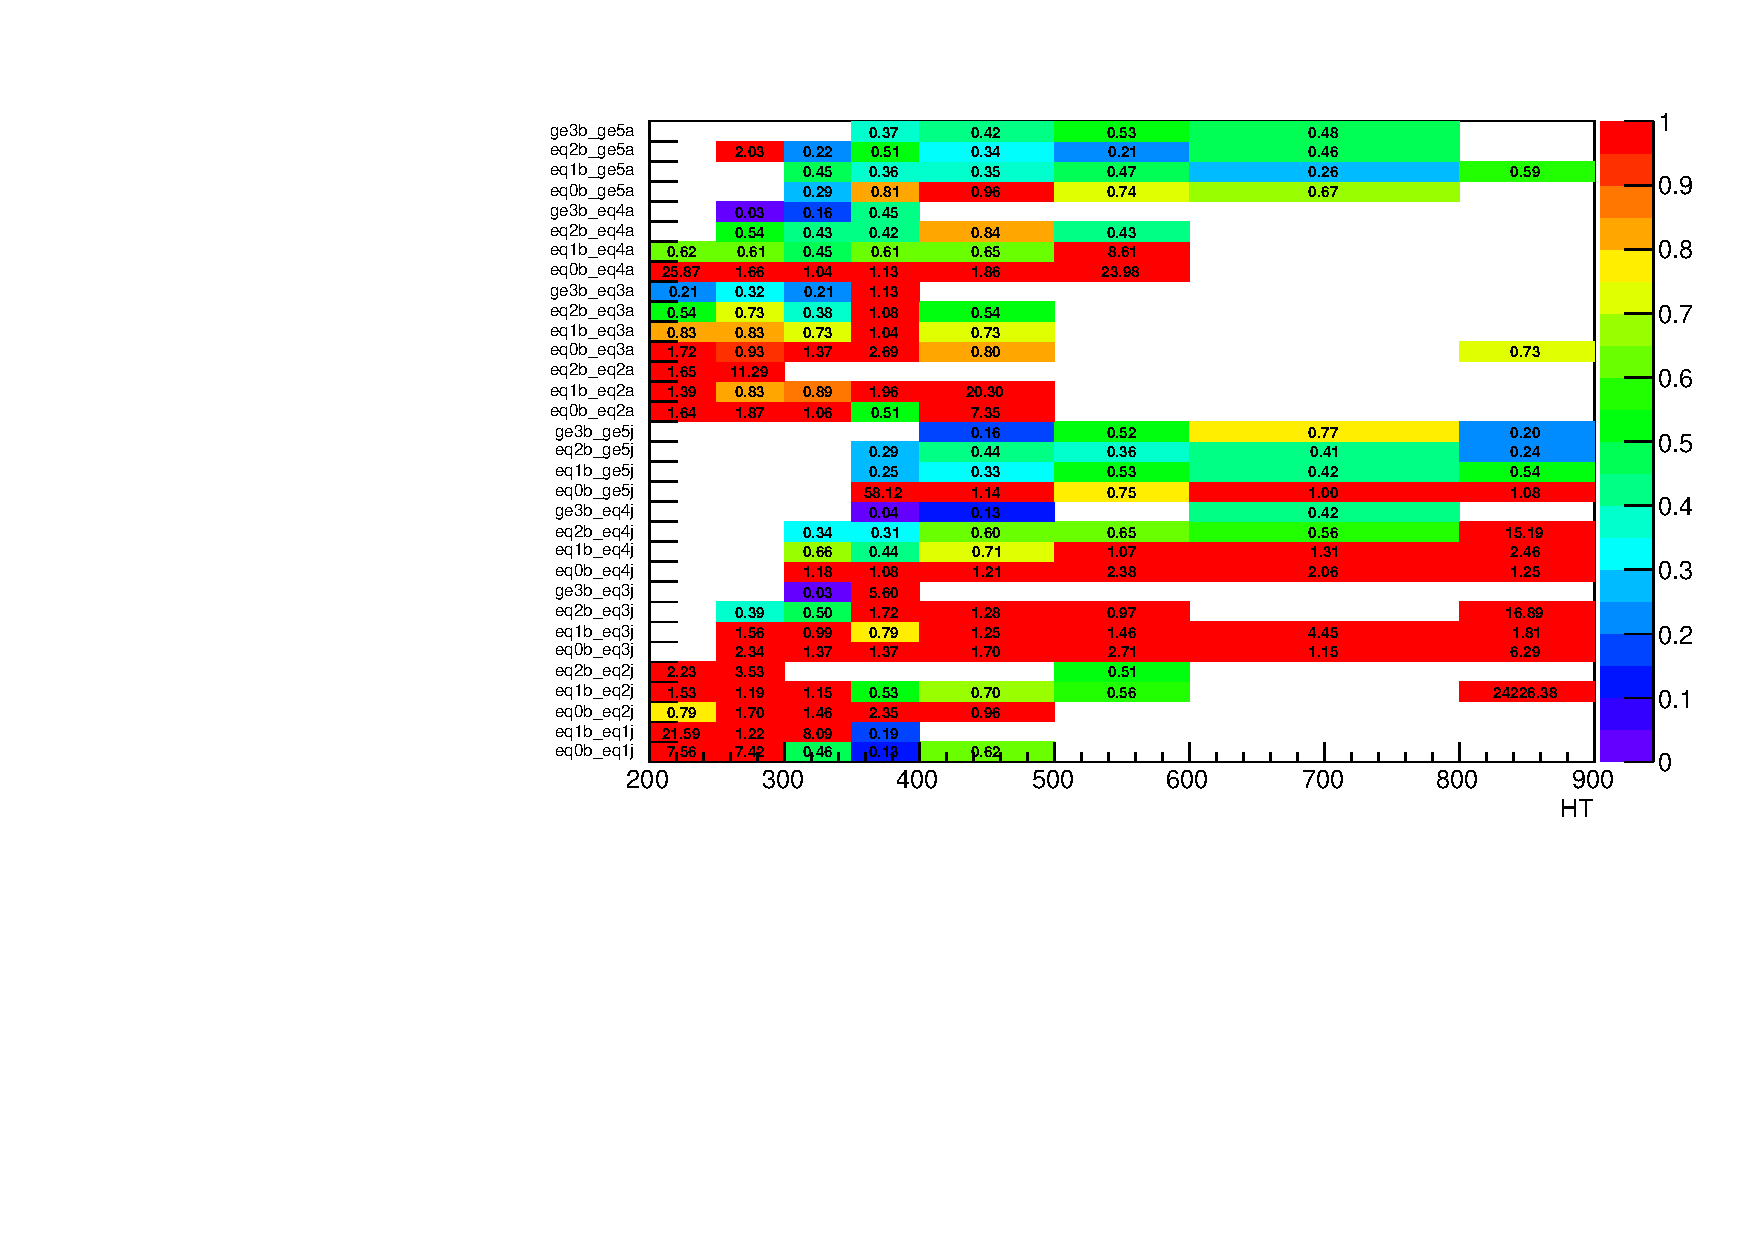
\includegraphics[width=0.5\textwidth]{figures/susyResults/doubleRatio_SingleMu_SMS-T2tt_mStop-250_mLSP-50_25ns}
%            \label{fig:contamination_T2tt_doubleRatio}
%        }
%        \caption{Characterisation of signal acceptance and contamination in the
%            signal and \mj control regions, respectively, for the benchmark
%            model T2tt (250,50).}
%        \label{fig:contamination_T2tt}
%    \end{center}
%\end{figure}

%The effect of signal contamination can be sizeable in these particular scenario
%for T2tt, as shown in Fig.~\ref{fig:contamination_T2tt_doubleRatio}, where in
%the most sensitive bins (high \nb, high \nj) the contribution of the control
%region sensitivity is comparable to the one of the signal region. However this
%is not an issue in the analysis, as the potential for signal contamination in
%all control samples is fully accounted for in the likelihood model used to
%extract the statistical interpretation (see Sec.~\ref{sec:likelihood}).
%
%The level of contamination for the \mmj sample is smaller still due to the
%requirement of a second muon.

\subsection{Systematic uncertainties on signal efficiency times acceptance}
\label{sec:sig-syst}
The following sources of systematic uncertainty are propagated to the signal
acceptance and shape, according to the recommendations agreed on within the
collaboration. Relative effect on the yields are presented in
Tab.~\ref{tab:sig-systematics} for some benchmark models.

\begin{itemize}
    \item Luminosity: 2.6\%, taken as correlated across all bins.
    \item Trigger: conservatively, the size of the inefficiency is taken as
        systematic variation where not in the plateau (see Sec.~\ref{sec:triggers}).
    \item MC statistics:  uncorrelated bin-by-bin uncertainty, affecting the
        shape of the signal.
    \item Pileup reweighting: 5.0\% uncertainty on the minimum bias cross section
        (see Sec.~\ref{sec:pileup-reweighting}).
    \item b-tag efficiency: uncertainty on the FullSim and FastSim b-tag scale
        factor is propagated and taken as correlated across the bins.
    \item Lepton efficiency: uncertainty on the lepton scale factors is
        propagated and taken as correlated across the bins.
    \item Jet energy scale: uncertainty on the jet energy corrections is
        propagated and taken as correlated across the bins.
    \item Initial State Radiation (ISR): Reweighting of the $N_{\text{isr}}$
        distribution. The systematic is taken as half the corrections.
\end{itemize}

\begin{table}[h!]
    \caption{Representative range taken from the $16\%$ and $84\%$ percentiles
        of the uncertainty across the analysis bins for each source of signal
        systematic. Two benchmark point are chosen for each model, corresponding
        to ``compressed'' and ``uncompressed'' scenarios, i.e. with small and
        large mass splitting between the mother particle and the LSP. A third
        benchmark is chosen for T2tt for the $W$ corridor.}
    \label{tab:sig-systematics}
    \centering
    \begin{tabular}{ ccccccccc }
        \hline \hline
        Model & ($m_{\mathrm{Susy}},m_{\mathrm{LSP}}$) & Luminosity & ISR & JEC & PU & b-tag & Trigger & MC stat. \\ \hline
        \multirow{2}{*}{T1bbbb}
            & (1900,100)  & 2.6\% & 2-6\%  & 3-6\%  & 7-11\% & 7-12\% & 3-4\% & 11-19\% \\ 
            & (1300,1100) & 2.6\% & 2-11\% & 3-11\% & 5-9\%  & 2-5\%  & 1-3\% & 11-22\% \\
        \hline
        \multirow{2}{*}{T2tt}
            & (1000,50) & 2.6\% & 3-7\%   & 5-12\% & 6-10\%  & 1-6\%  & 1-4\%  & 14-26\% \\ 
            & (450,200) & 2.6\% & 4-12\%  & 5-15\% & 10-15\% & 3-9\%  & 3-6\%  & 6-19\%  \\
            & (250,150) & 2.6\% & 13-27\% & 8-22\% & 12-28\% & 6-20\% & 6-21\% & 10-24\% \\
        \hline
        \multirow{1}{*}{T2cc}
            & (500,480) & 2.6\% & 4-17\% & 5-13\% & 5-12\% & 1-4\% & 2-4\% & 7-19\% \\
        \hline
        \multirow{2}{*}{T2bb}
            & (1000,100) & 2.6\% & 1-8\%  & 4-11\% & 6-10\% & 1-5\% & 0-3\% & 14-24\% \\ 
            & (550,450)  & 2.6\% & 4-15\% & 4-15\% & 8-13\% & 2-6\% & 2-4\% & 9-22\%  \\
        \hline \hline
    \end{tabular}
\end{table}

\subsection{Exclusion limits}
\label{sec:susy_results}
In order to extract the signal contribution in the fit, the distribution of
events according to the \mht variable, encoded as template histograms, is used
as described in Sec.~\ref{sec:had-shape} and \ref{sec:likelihood}. \\
Upper limits on the cross section are computed using the $\text{CL}_{s}$
criterion \cite{CLsTechnique}. Asymptotic formulae \cite{AsymptoticFormulae} are
utilised to approximate the distribution of the test statistics. \\
All the statistical results are produced using the \textit{combine} tool,
provided within the HiggsAnalysis-CombinedLimit package \cite{Combine}.

In Fig. ~\ref{fig:T1bbbb}-\ref{fig:T2bb} (top) the 95\% C.L. upper limits on the
cross section are shown in the $(m_{\mathrm{Susy}},m_{\mathrm{LSP}})$ plane for
the models considered in this interpretation. These results correspond to
35.9~\ifb of integrated luminosity. The exclusion contour is also shown together
with $\pm1\sigma$ (and $\pm2\sigma$ for the expected exclusion) uncertainty.
The band around the expected exclusion reflects the experimental uncertainty,
while the band around the observed exclusion correspond to the theoretical
uncertainty on the signal cross section.\\

In Fig.~\ref{fig:T1bbbb}-\ref{fig:T2bb} (bottom left) the signal acceptance
for each mass point in the SMS scan.

In Fig.~\ref{fig:T1bbbb}-\ref{fig:T2bb} (bottom left) each mass point is
assigned a group of 4 jet categories in descending order of sensitivity. The
total number of mass points with the same 4 most sensitive jet categories is
noted. In T1bbbb, the 4 most sensitive jet categories are the symmetric high jet
multiplicities (eq5j, ge6j, eq4j, eq3j), with the asymmetric category playing
a role in the compressed spectrum (ge6j, eq5j, ge2a, eq4j). The sensitive
categories for T2tt and T2cc are similar to T1bbbb: symmetric high jet
multiplicities with the asymmetric topology playing a role in the compressed
region. In T2bb, the sensitivity is driven by symmetric moderate jet
multiplicities (eq2j, eq3j, eq4j, eq5j) in the uncompressed region and the high
jet multiplicities in the compressed region (eq4j, eq5j, ge6j, ge2a).

The models are grouped according to the following categorisation:
\begin{itemize}
    \item \textbf{Gluino-mediated production of off-shell (decoupled) 3rd generation squarks}:
        gluino pair production followed by 3-body decay to $t\bar{t}\chiz$,$q\bar{q}\chiz$,$b\bar{b}\chiz$.
        It includes T1bbbb, T1qqqq and T1tttt.
    \item \textbf{Direct production of 3rd generation squarks}: stop/sbottom
        pair production, with several possibility for the decay
        (see Tab.~\ref{tab:simplified-models}). It includes T2tt, T2cc, T2bb and T2qq.
\end{itemize}

%Summary exclusion plots according to this categorisation are presented in
%Fig.~\ref{fig:summary-excl-plots}.

\newpage
\begin{figure}[h!]
    \begin{center}
        \subfigure[T1bbbb: Upper limit on the cross section in the mass plane]{
            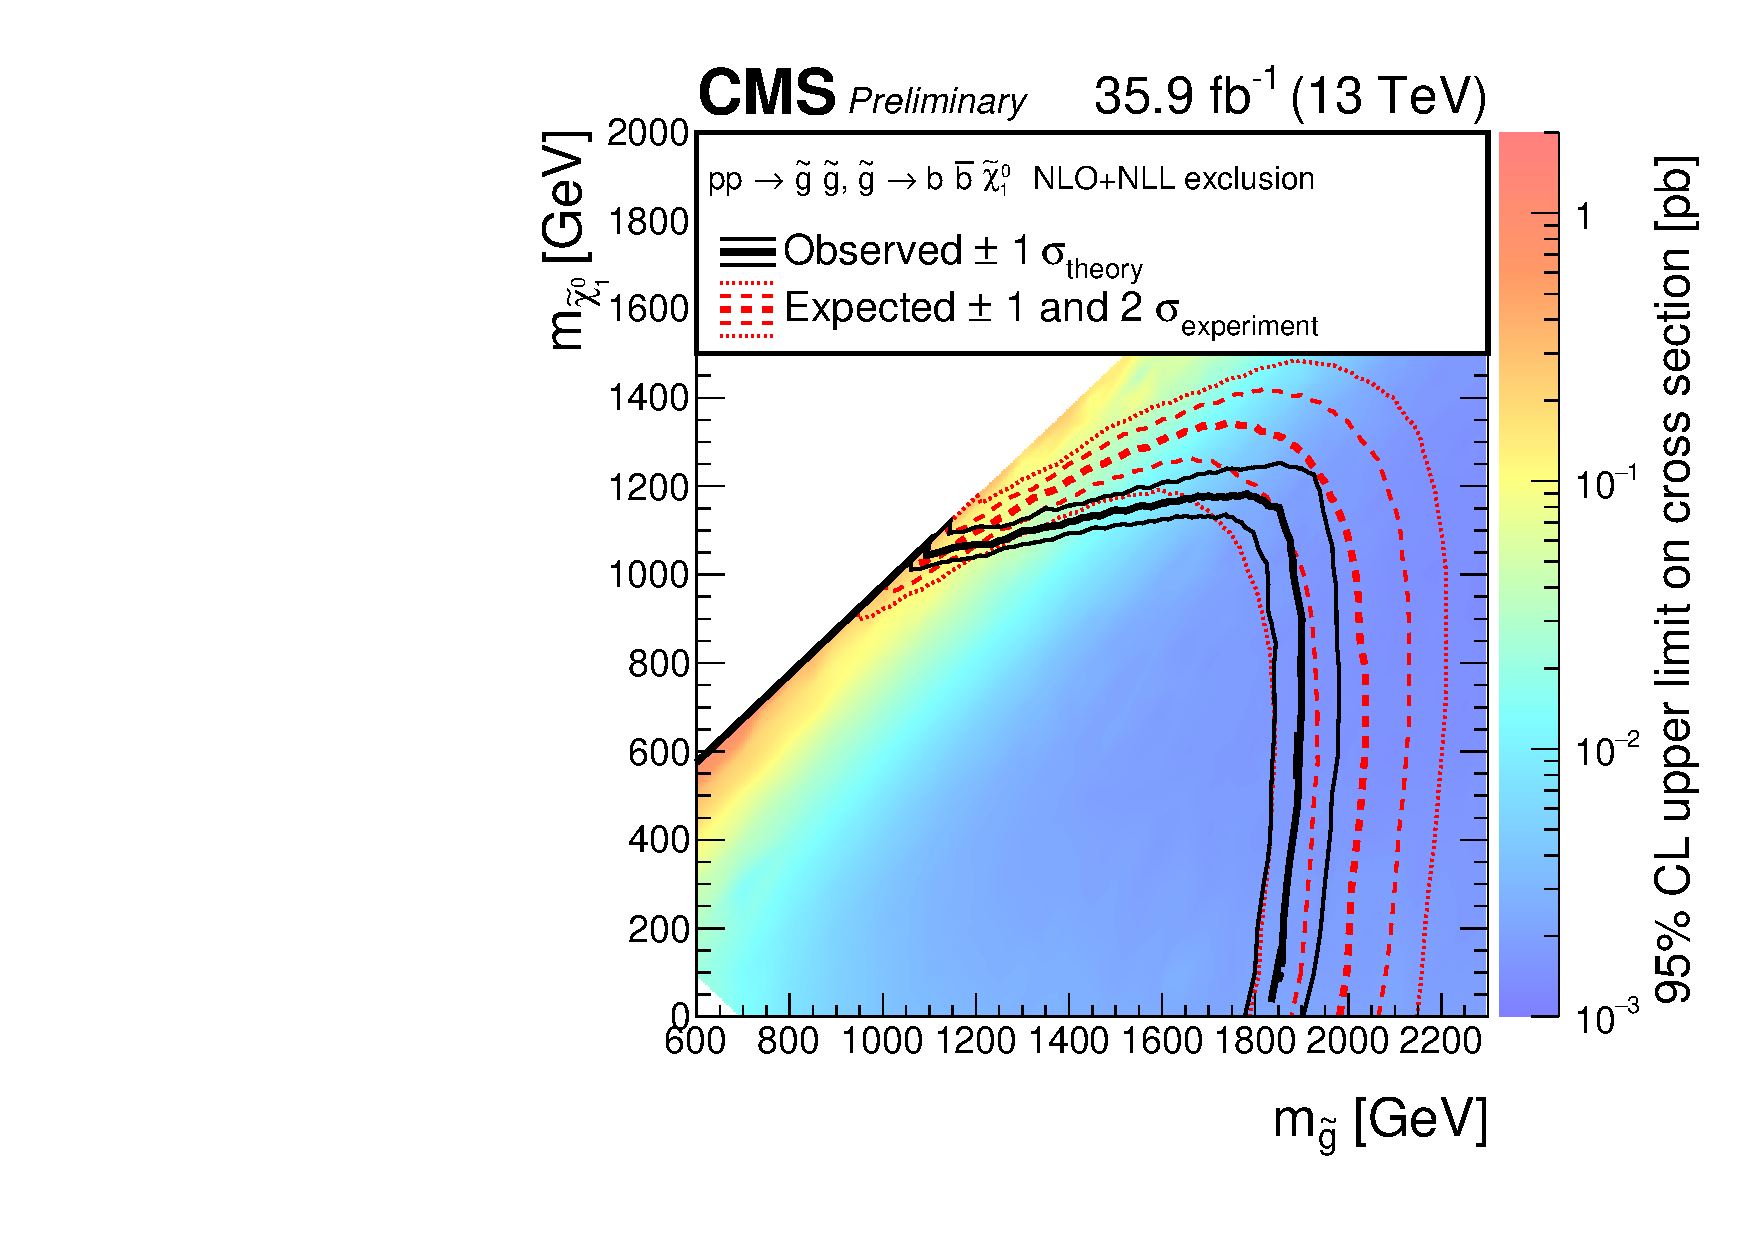
\includegraphics[width=0.6\textwidth]{figures/susyResults/T1bbbbXSEC}
            \label{fig:T1bbbb_excl}
        } \\
        \subfigure[T1bbbb: $\epsilon_{sig}$]{
            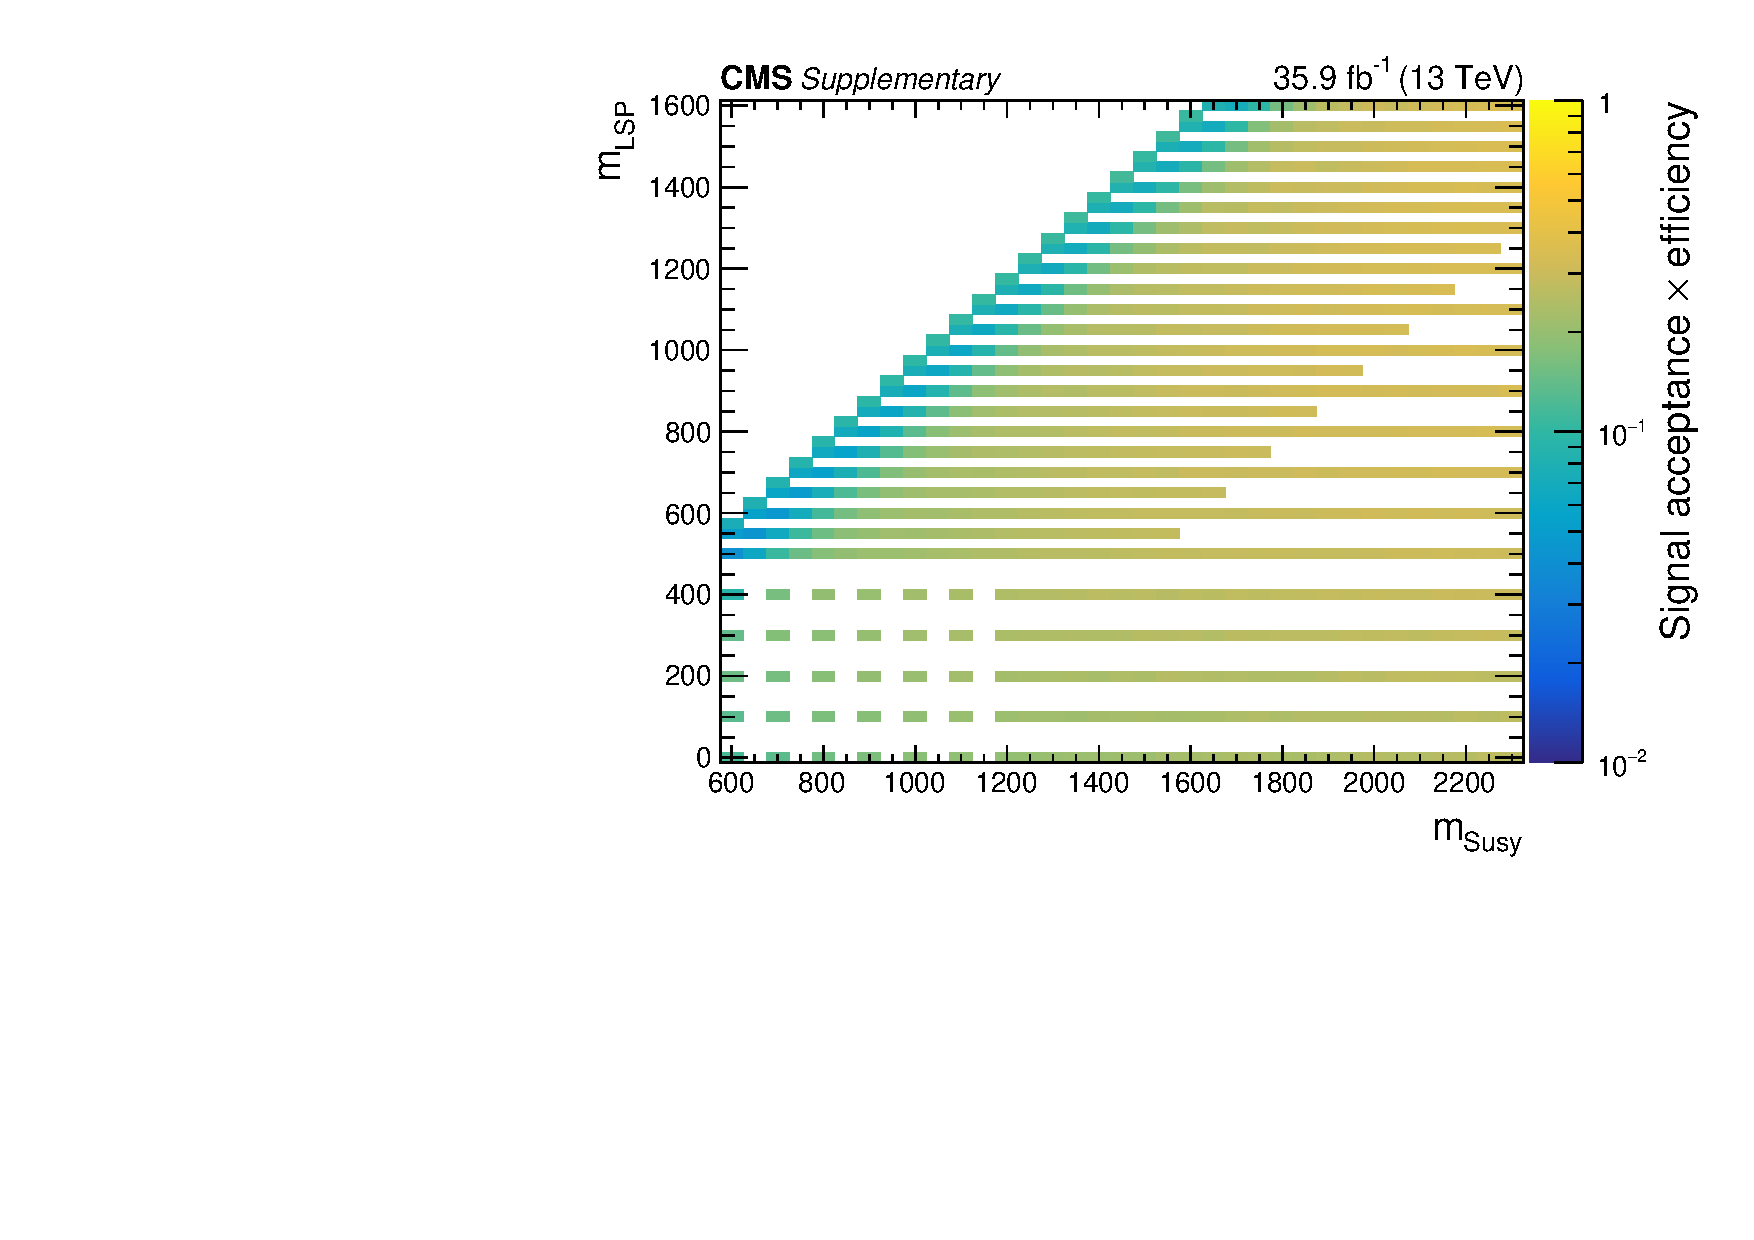
\includegraphics[width=0.45\textwidth]{figures/susyResults/T1bbbb_effs}
            \label{fig:T1bbbb_eff}
        } ~~
        \subfigure[T1bbbb: Most sensitive categories]{
            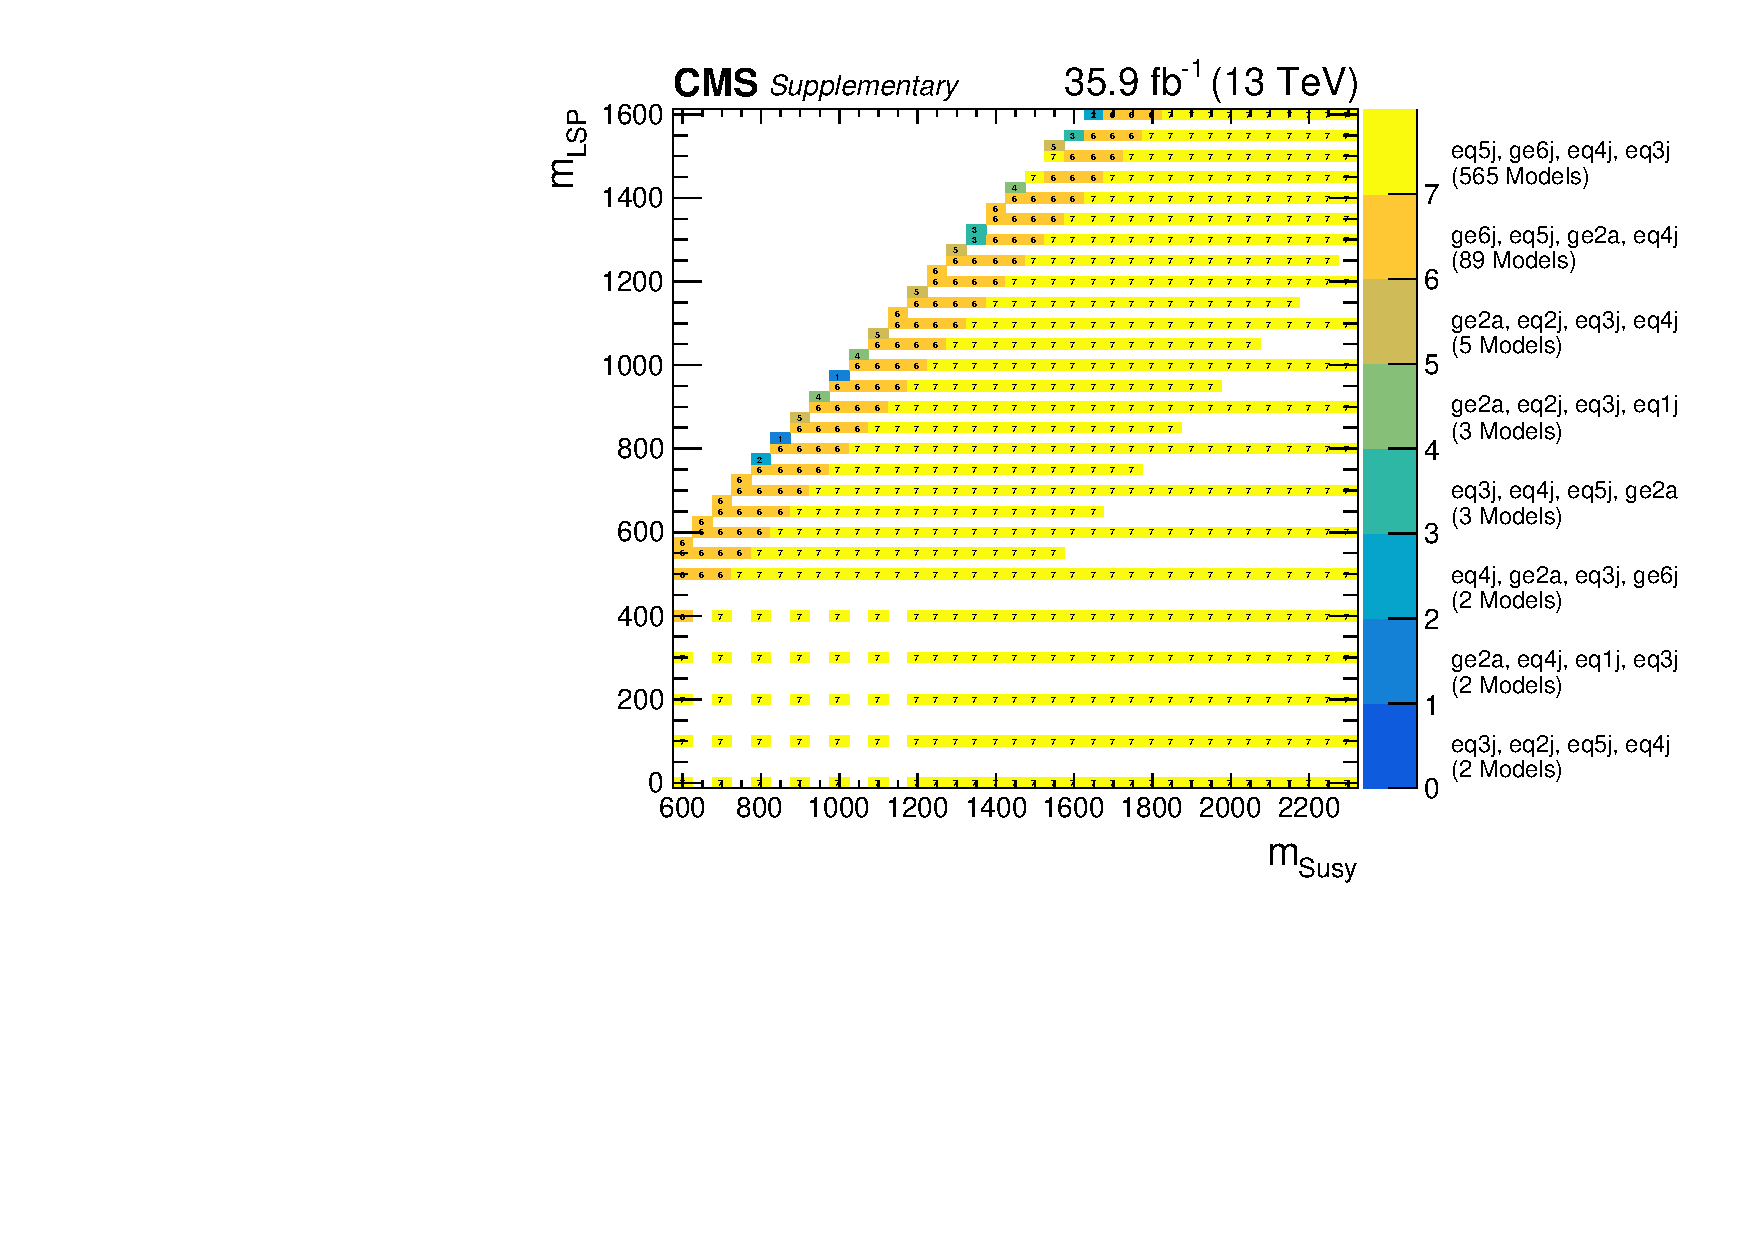
\includegraphics[width=0.45\textwidth]{figures/susyResults/T1bbbb_bitMap}
            \label{fig:T1bbbb_bitMap}
        } ~~
        \caption{Top: the 95\% C.L. observed upper limit on the cross section
            (histogram), with the expected (solid black line) observed
            (solid red line) exclusion contours. Bottom left: signal acceptance
            including all jet categories. Bottom right: bitmap representing the
            most sensitive jet categories for each mass point.}
        \label{fig:T1bbbb}
    \end{center}
\end{figure}

\newpage
\begin{figure}[h!]
    \begin{center}
        \subfigure[T1qqqq: Upper limit on the cross section in the mass plane]{
            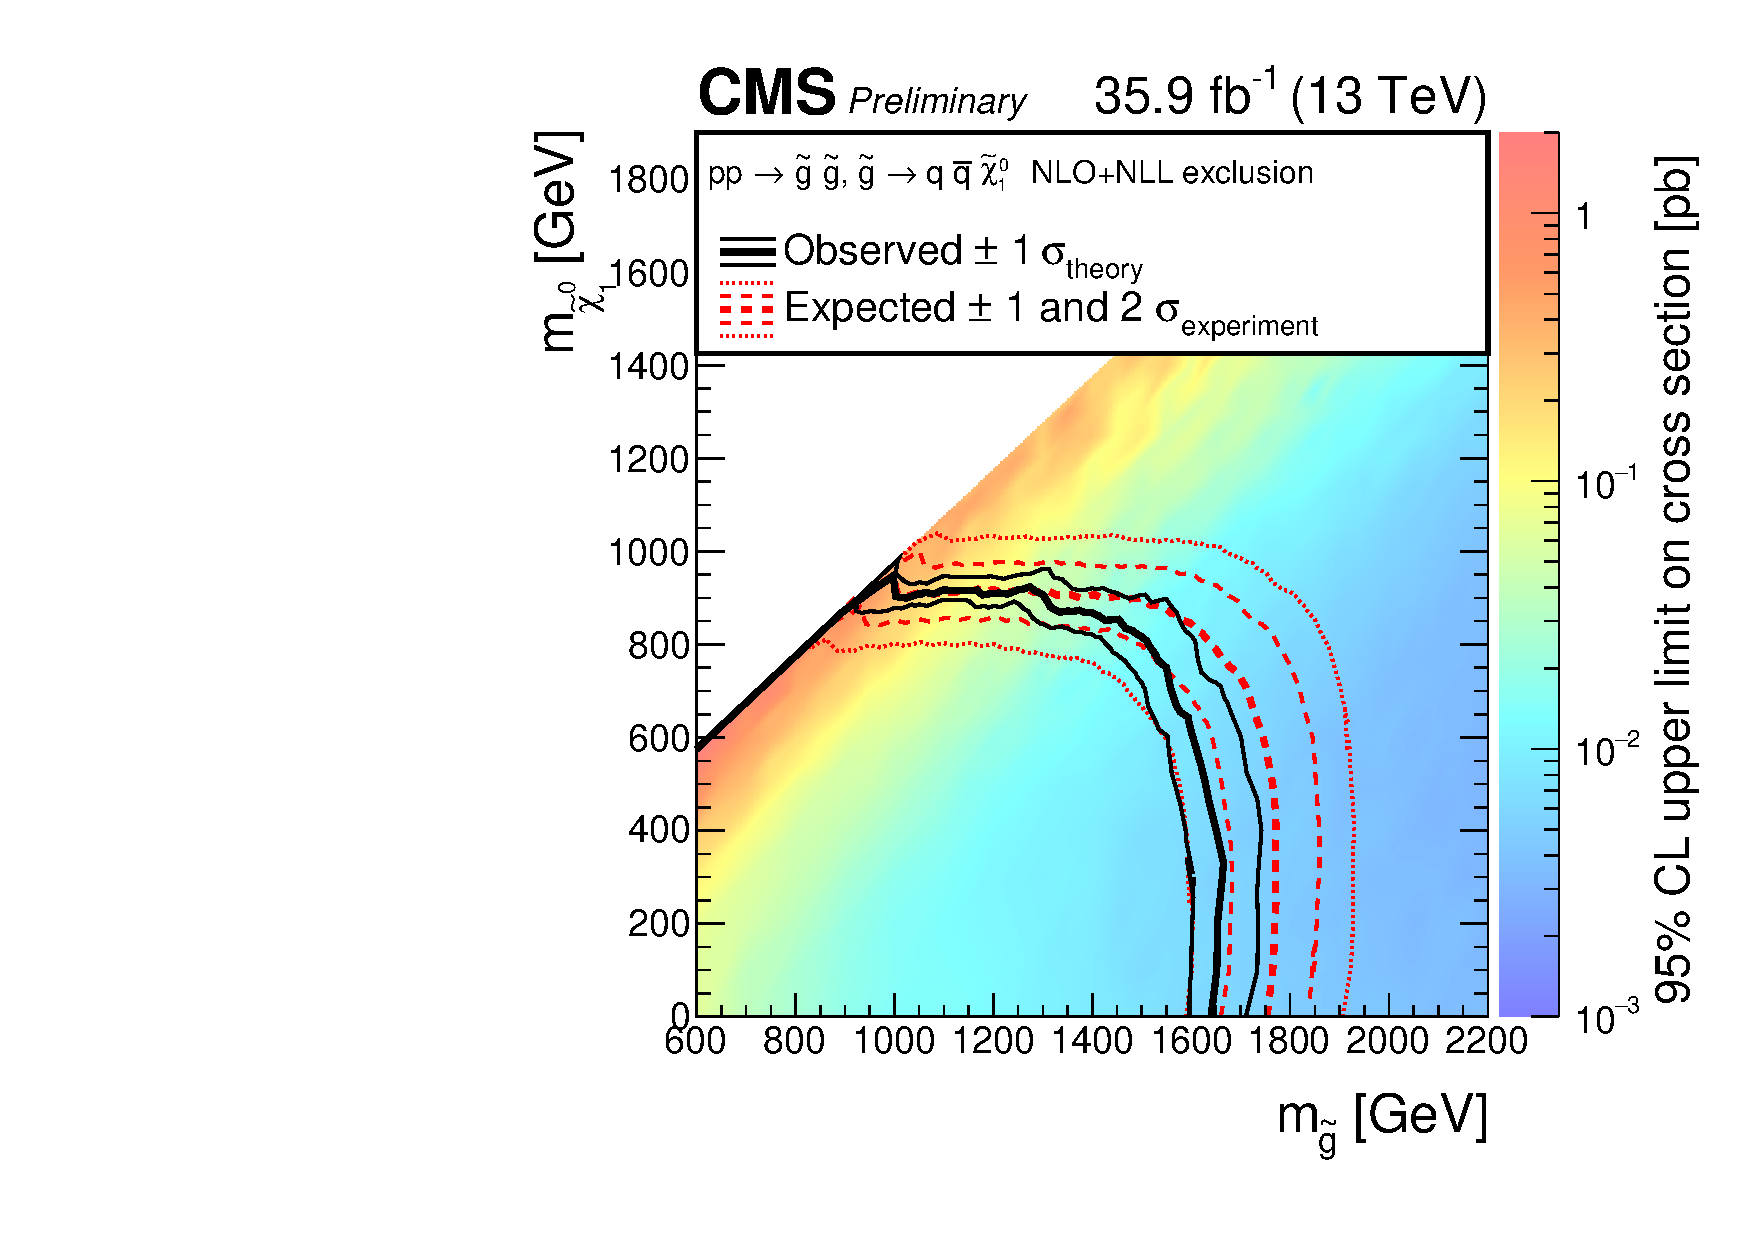
\includegraphics[width=0.6\textwidth]{figures/susyResults/T1qqqqXSEC}
            \label{fig:T1qqqq_excl}
        } \\
        \subfigure[T1qqqq: $\epsilon_{sig}$]{
            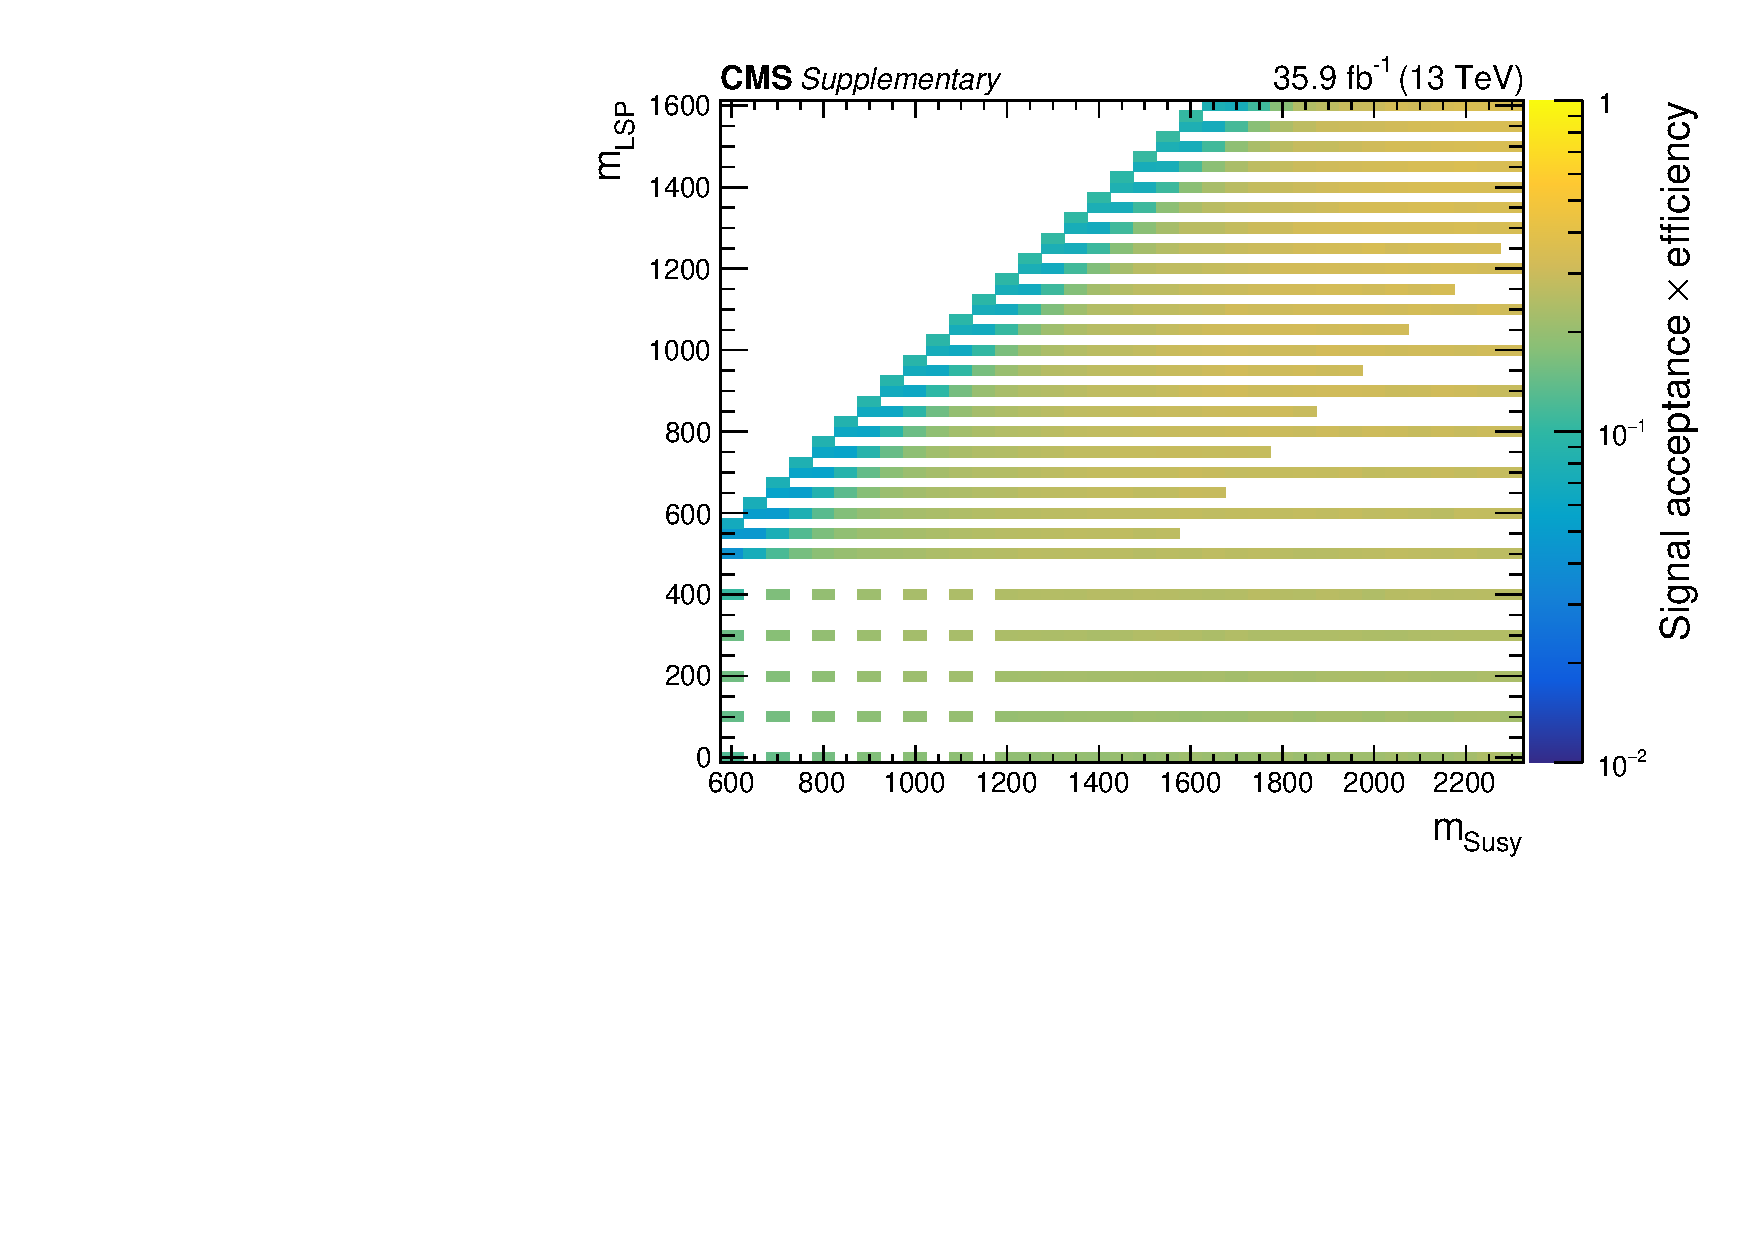
\includegraphics[width=0.45\textwidth]{figures/susyResults/T1qqqq_effs}
            \label{fig:T1qqqq_eff}
        } ~~
        \subfigure[T1qqqq: Most sensitive categories]{
            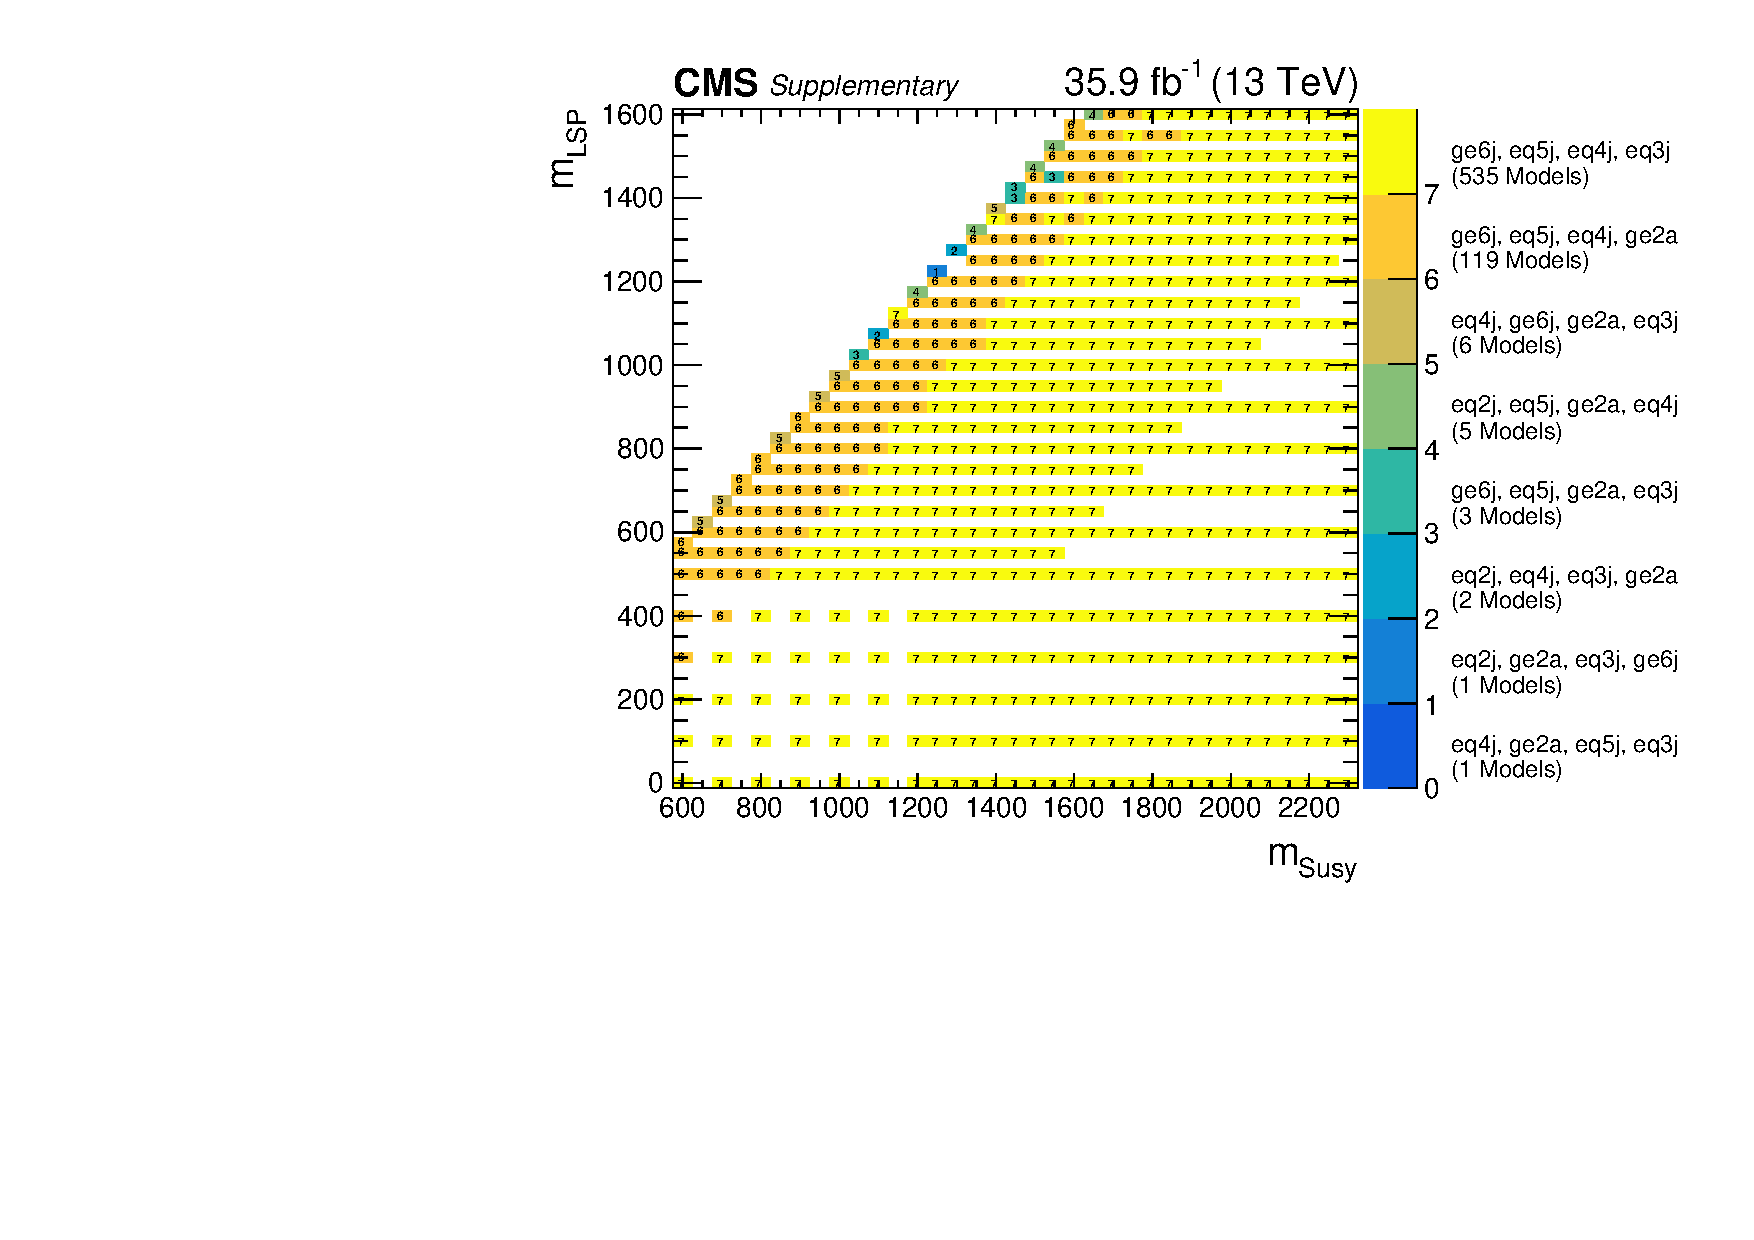
\includegraphics[width=0.45\textwidth]{figures/susyResults/T1qqqq_bitMap}
            \label{fig:T1qqqq_bitMap}
        } ~~
        \caption{Top: the 95\% C.L. observed upper limit on the cross section
            (histogram), with the expected (solid black line) observed
            (solid red line) exclusion contours. Bottom left: signal acceptance
            including all jet categories. Bottom right: bitmap representing the
            most sensitive jet categories for each mass point.}
        \label{fig:T1qqqq}
    \end{center}
\end{figure}

\newpage
\begin{figure}[h!]
    \begin{center}
        \subfigure[T1tttt: Upper limit on the cross section in the mass plane]{
            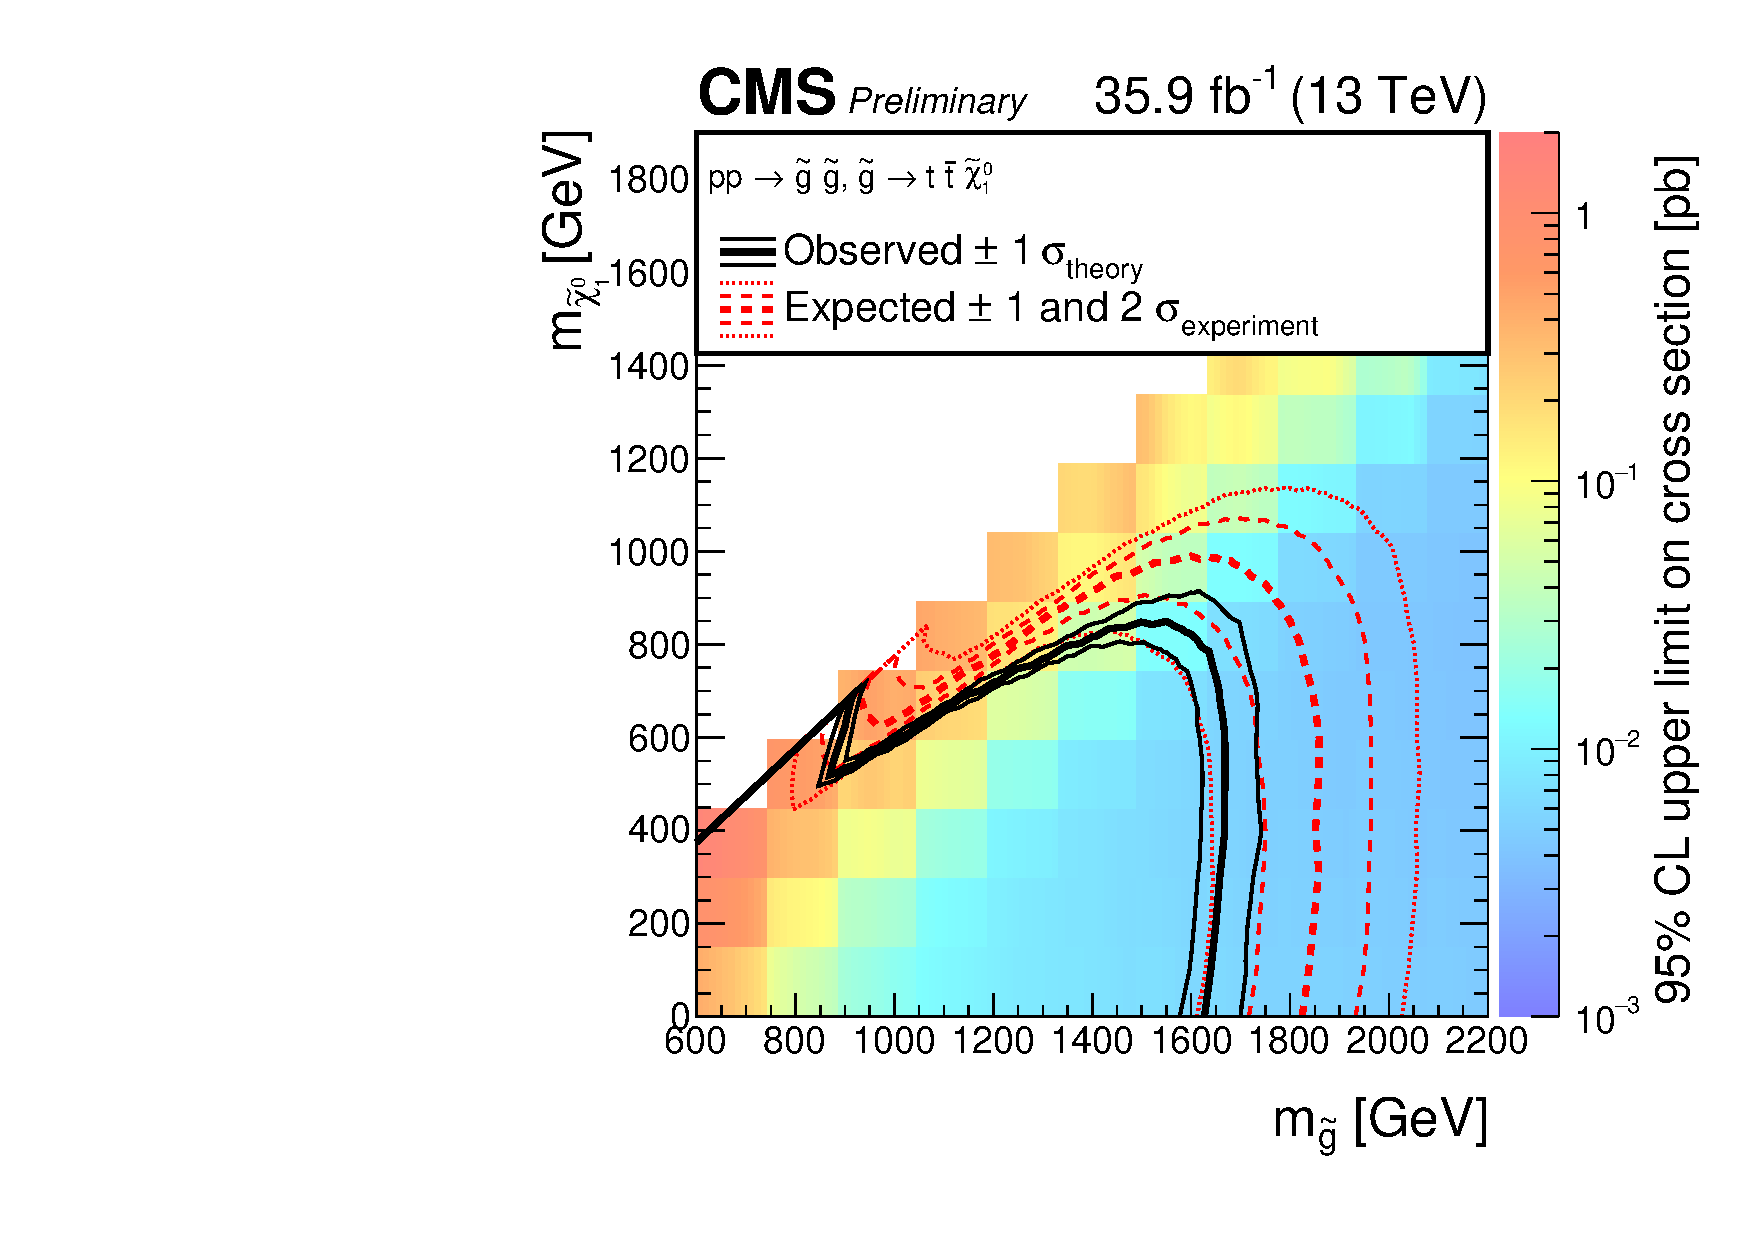
\includegraphics[width=0.6\textwidth]{figures/susyResults/T1ttttXSEC}
            \label{fig:T1tttt_excl}
        } \\
        \subfigure[T1tttt: $\epsilon_{sig}$]{
            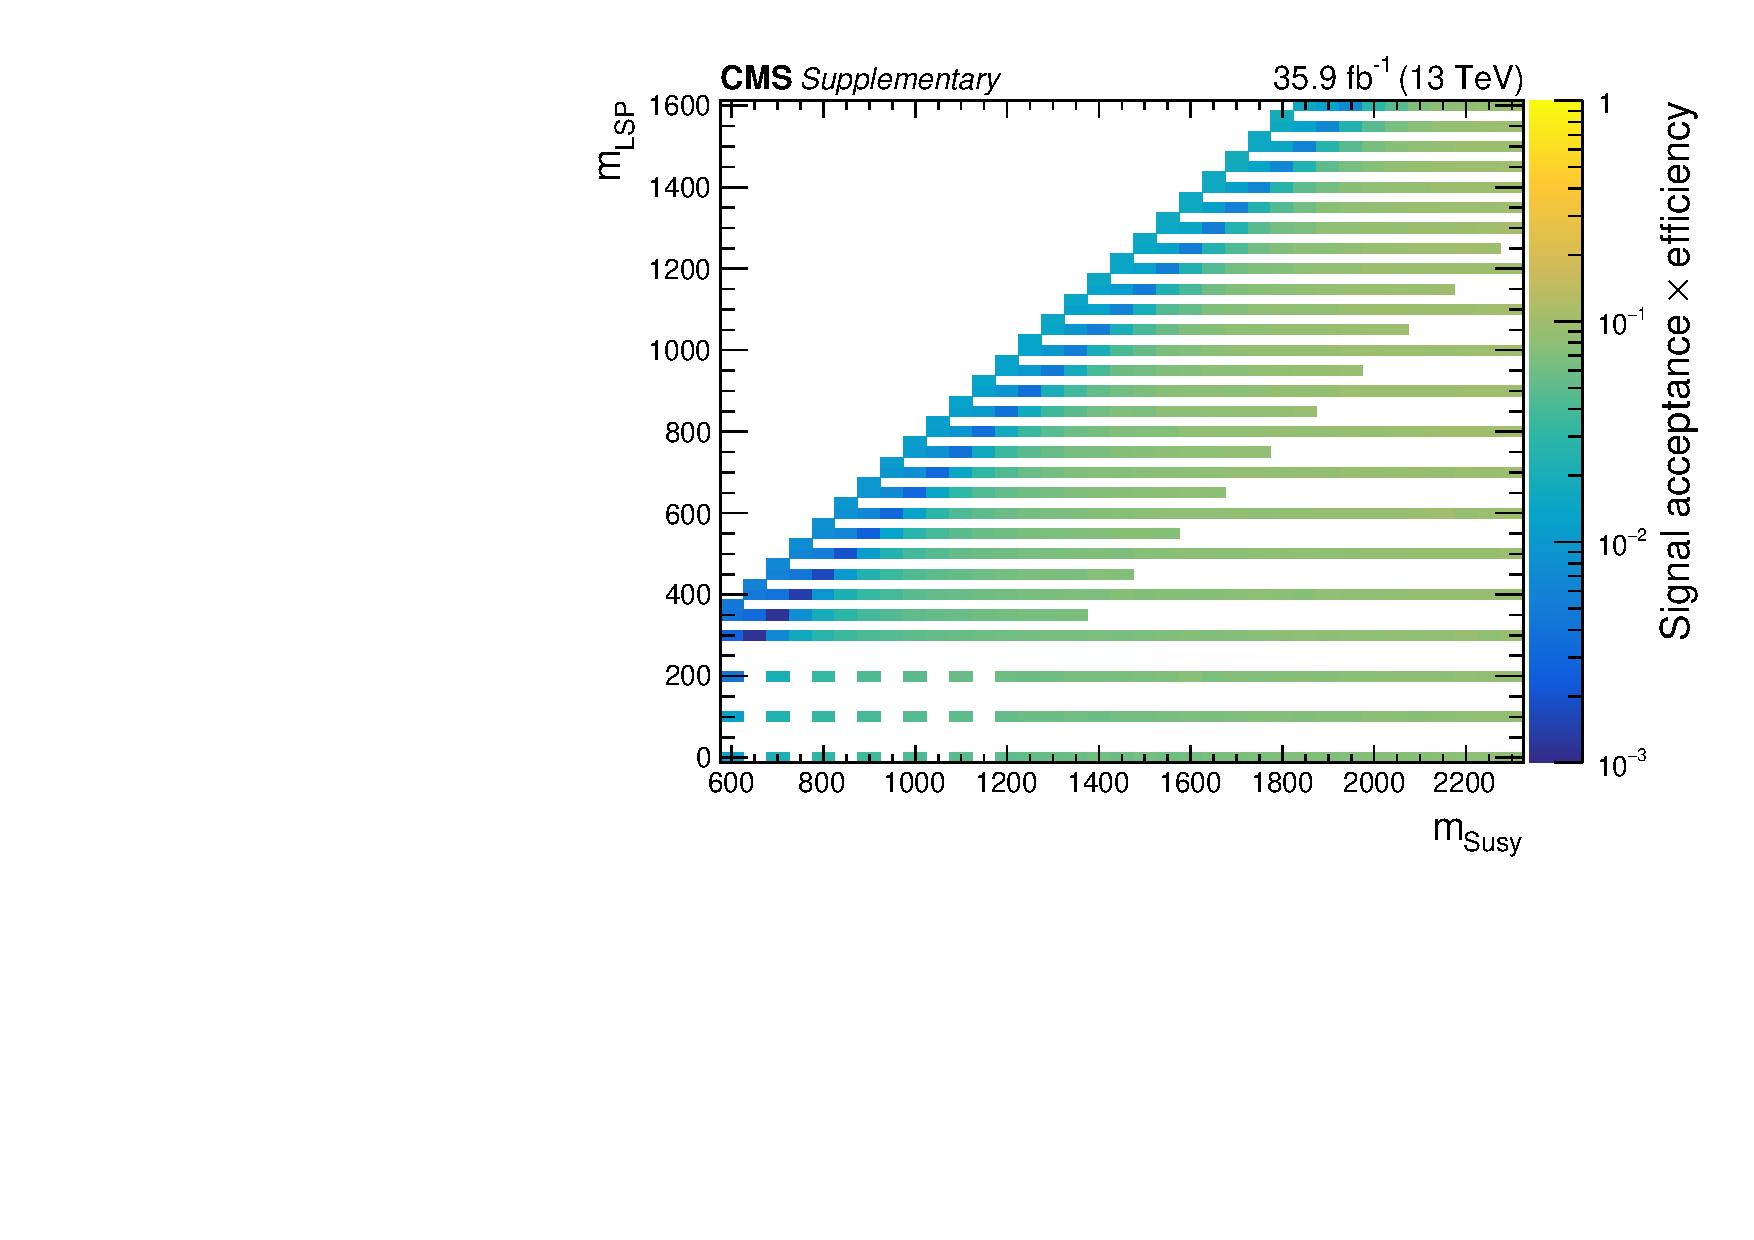
\includegraphics[width=0.45\textwidth]{figures/susyResults/T1tttt_effs}
            \label{fig:T1tttt_eff}
        } ~~
        \subfigure[T1tttt: Most sensitive categories]{
            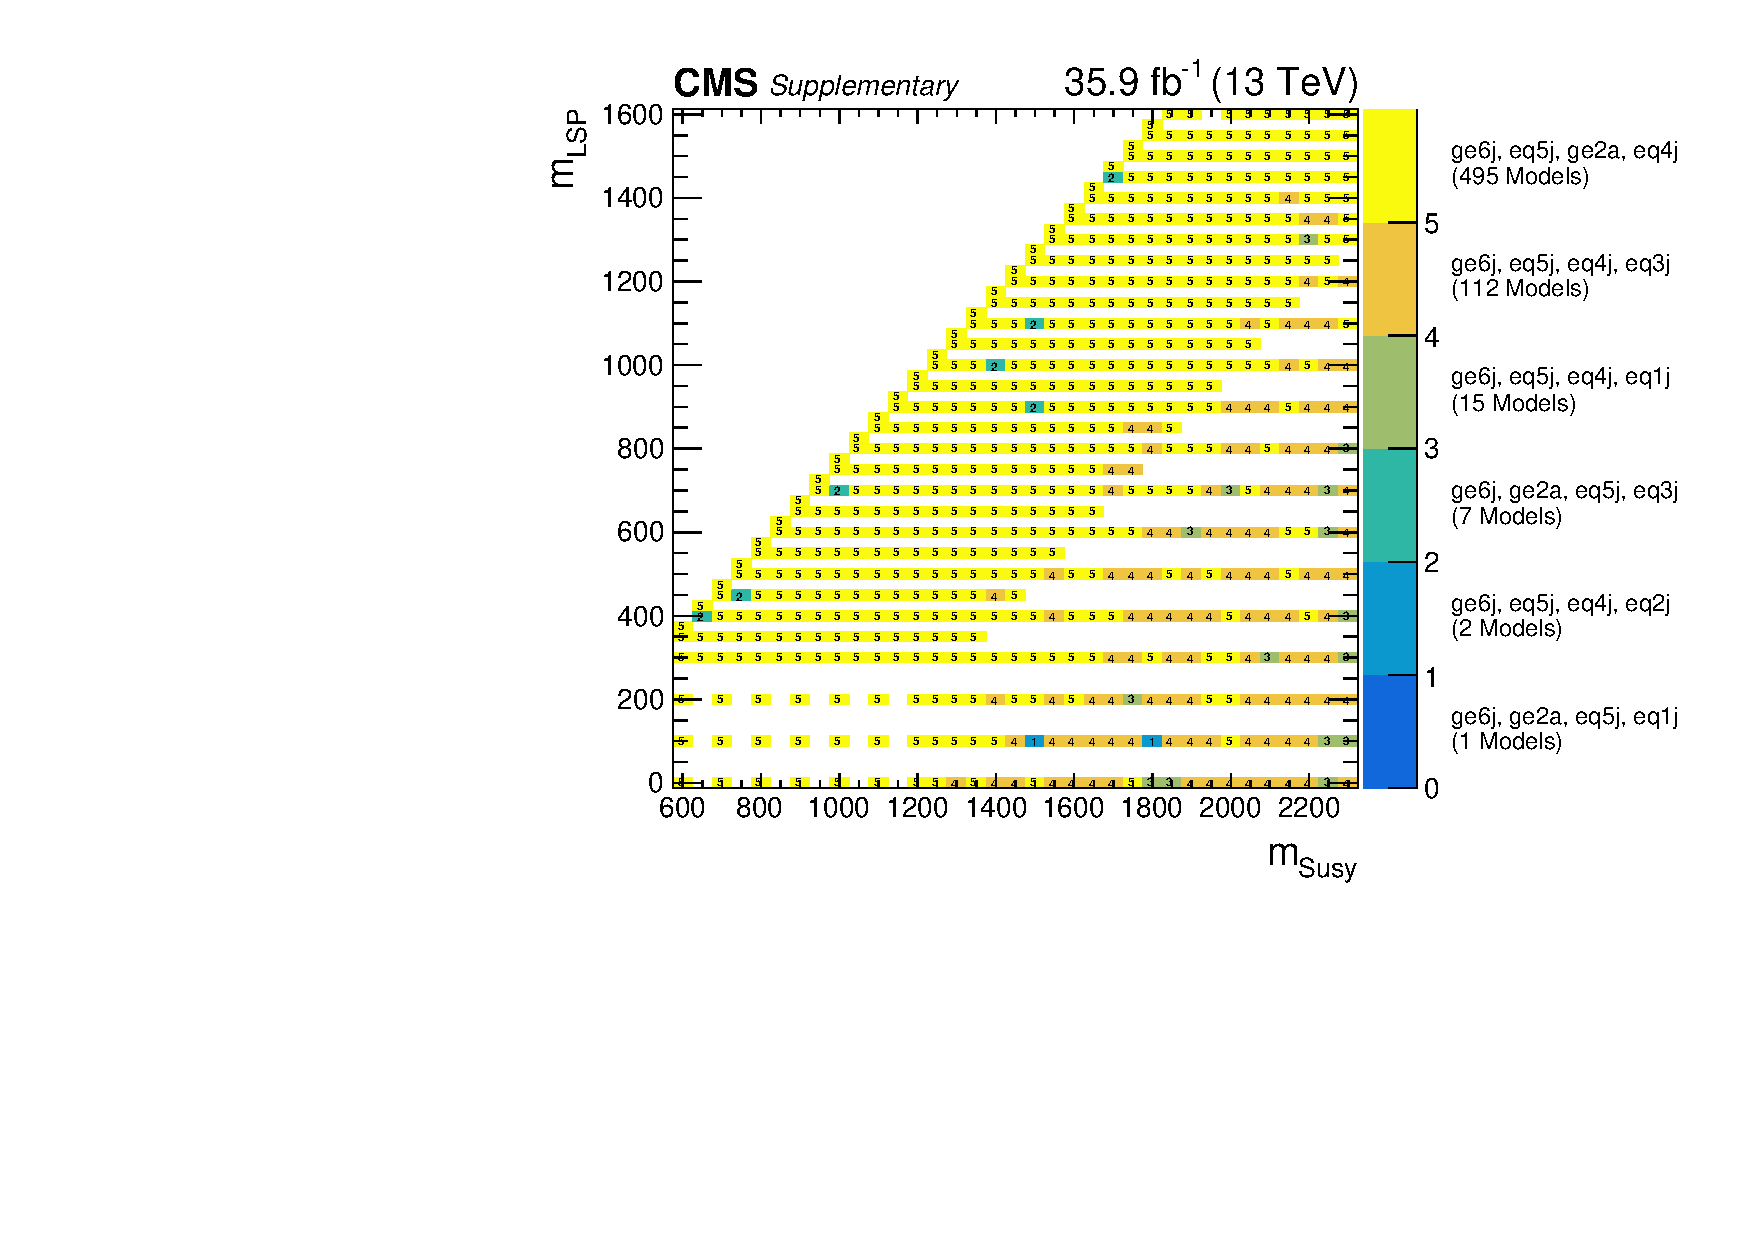
\includegraphics[width=0.45\textwidth]{figures/susyResults/T1tttt_bitMap}
            \label{fig:T1tttt_bitMap}
        } ~~
        \caption{Top: the 95\% C.L. observed upper limit on the cross section
            (histogram), with the expected (solid black line) observed
            (solid red line) exclusion contours. Bottom left: signal acceptance
            including all jet categories. Bottom right: bitmap representing the
            most sensitive jet categories for each mass point.}
        \label{fig:T1tttt}
    \end{center}
\end{figure}

\newpage
\begin{figure}[h!]
    \begin{center}
        \subfigure[T2tt: Upper limit on the cross section in the mass plane]{
            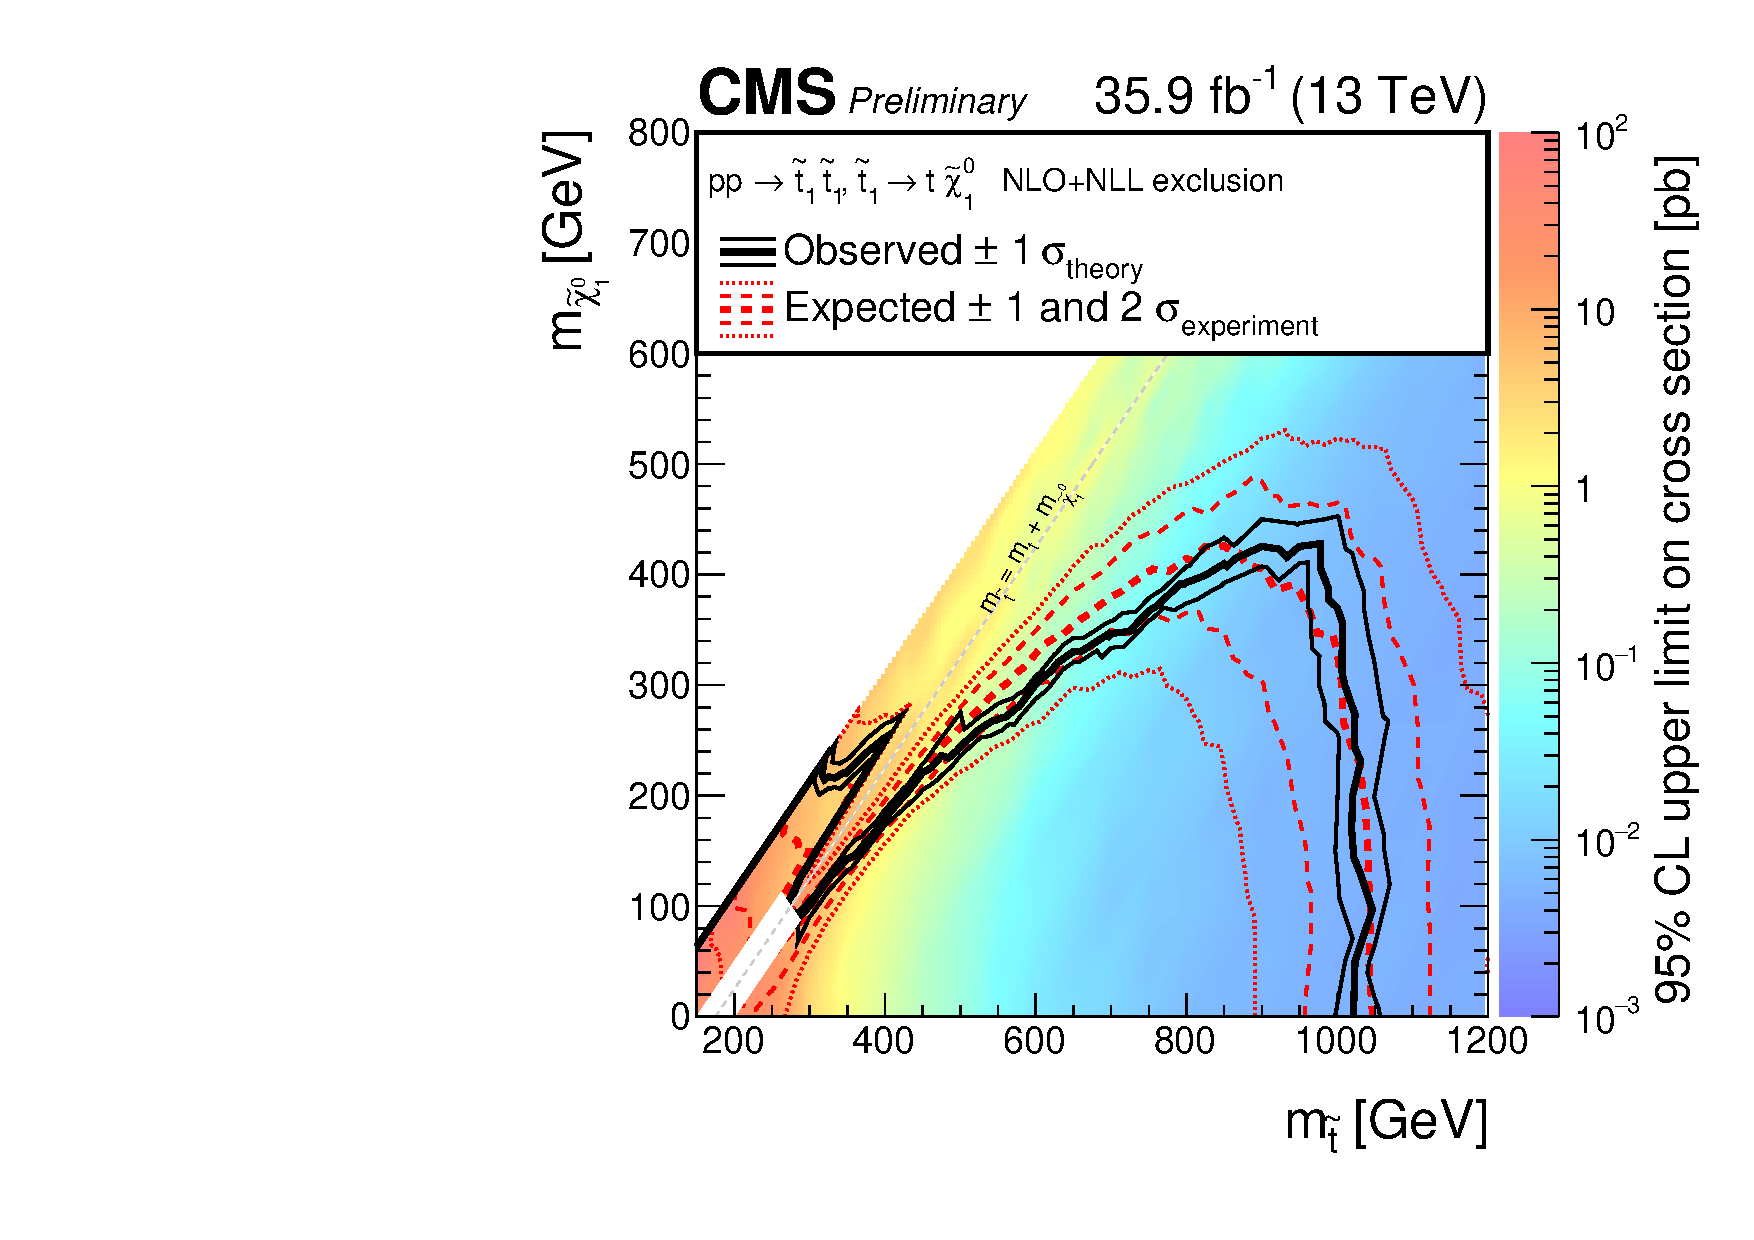
\includegraphics[width=0.6\textwidth]{figures/susyResults/T2ttXSEC}
            \label{fig:T2tt_excl}
        } \\
        \subfigure[T2tt: $\epsilon_{sig}$]{
            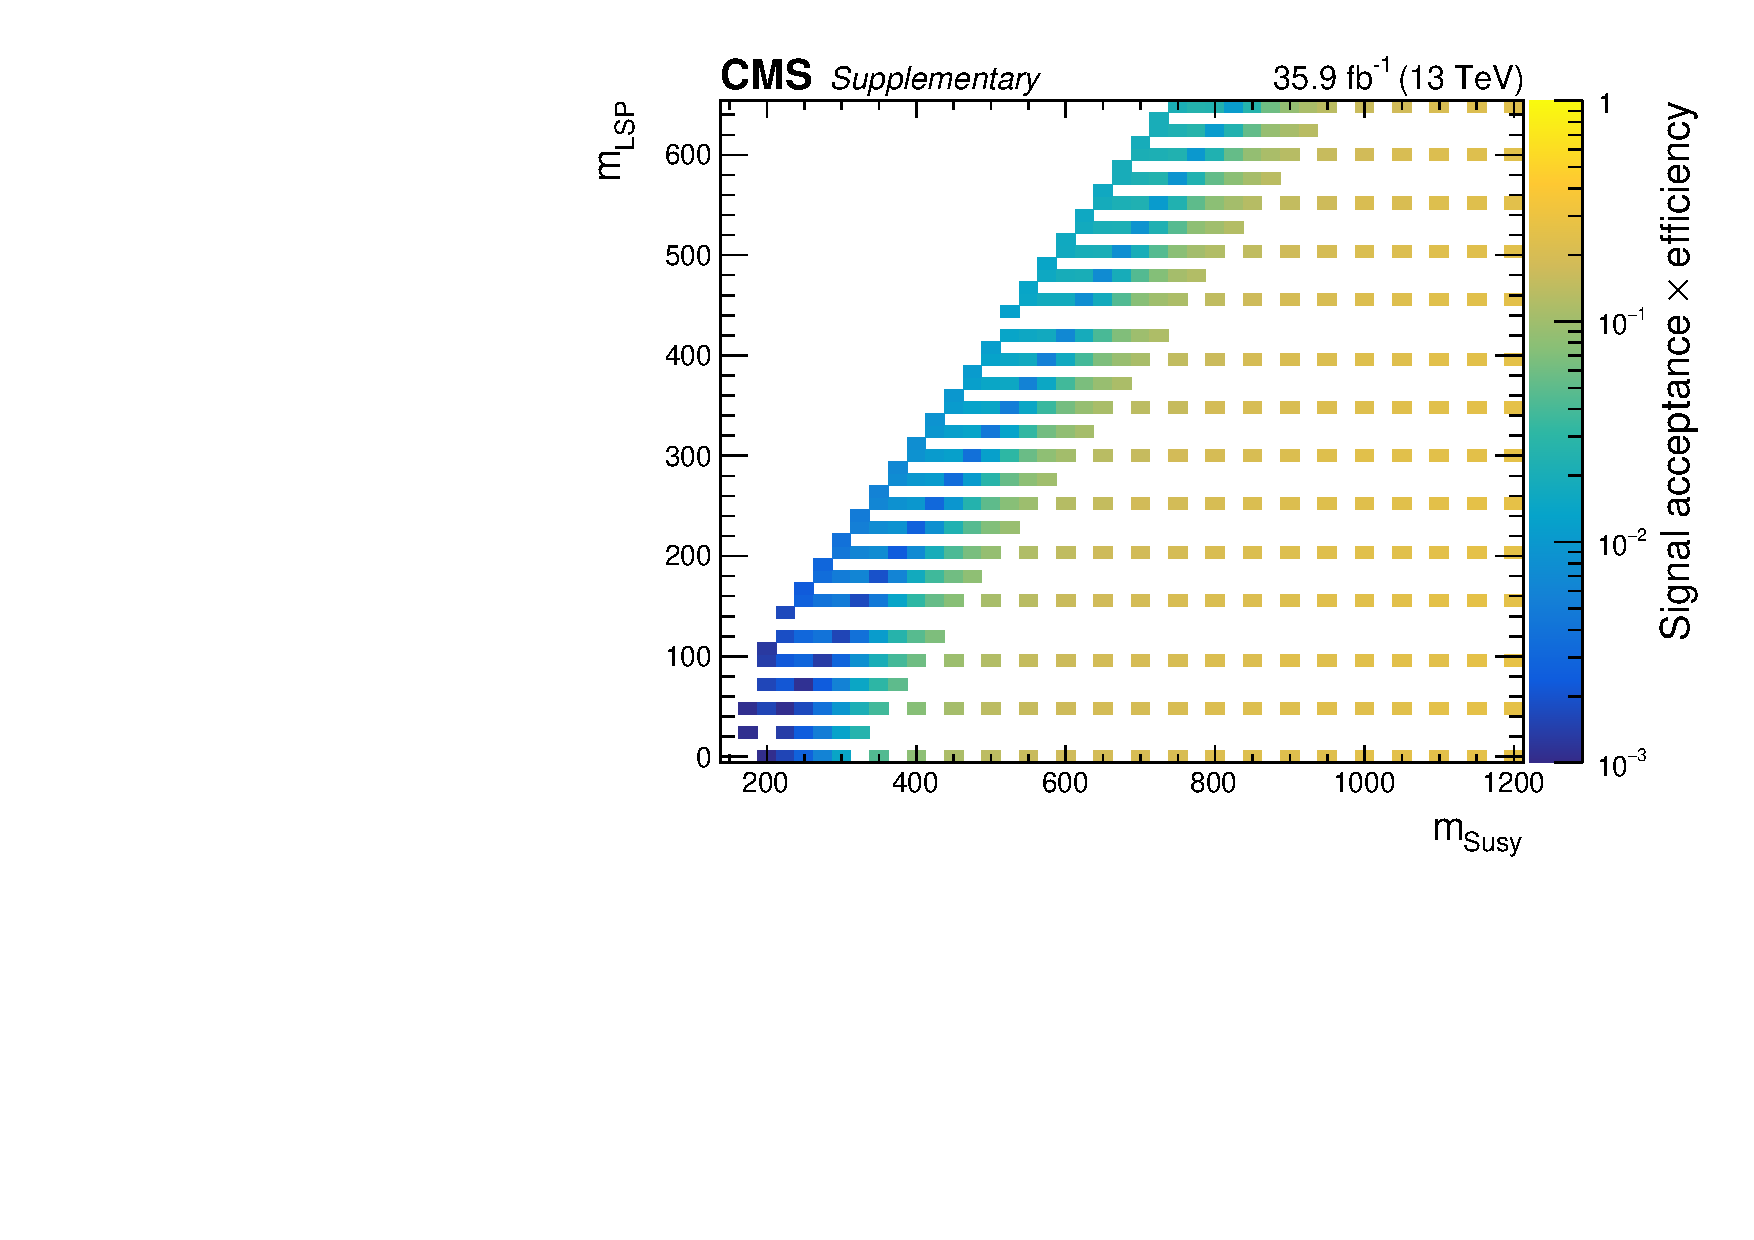
\includegraphics[width=0.45\textwidth]{figures/susyResults/T2tt_effs}
            \label{fig:T2tt_eff}
        } ~~
        \subfigure[T2tt: Most sensitive categories]{
            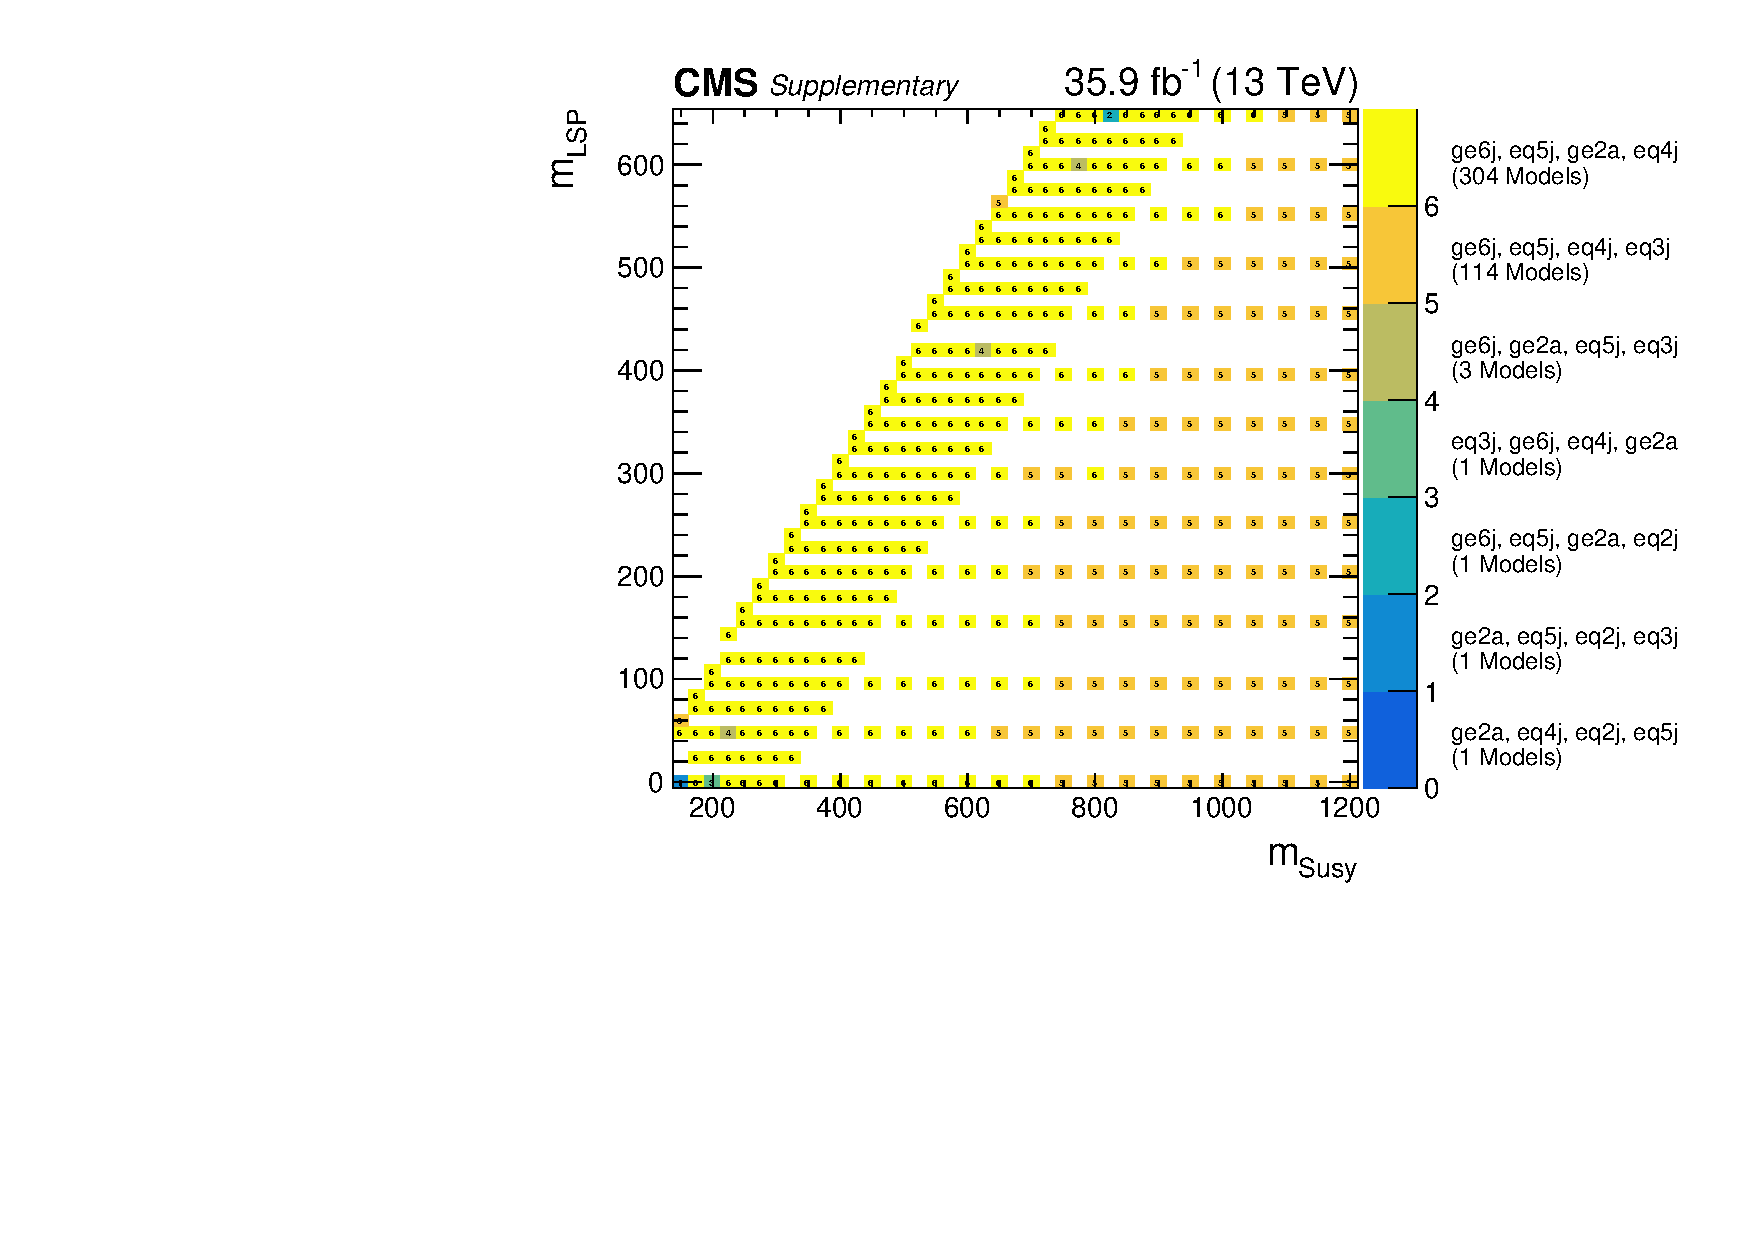
\includegraphics[width=0.45\textwidth]{figures/susyResults/T2tt_bitMap}
            \label{fig:T2tt_bitMap}
        } ~~
        \caption{Top: the 95\% C.L. observed upper limit on the cross section
            (histogram), with the expected (solid black line) observed
            (solid red line) exclusion contours. Bottom left: signal acceptance
            including all jet categories. Bottom right: bitmap representing the
            most sensitive jet categories for each mass point.}
        \label{fig:T2tt}
    \end{center}
\end{figure}

\newpage
\begin{figure}[h!]
    \begin{center}
        \subfigure[T2cc: Upper limit on the cross section in the mass plane]{
            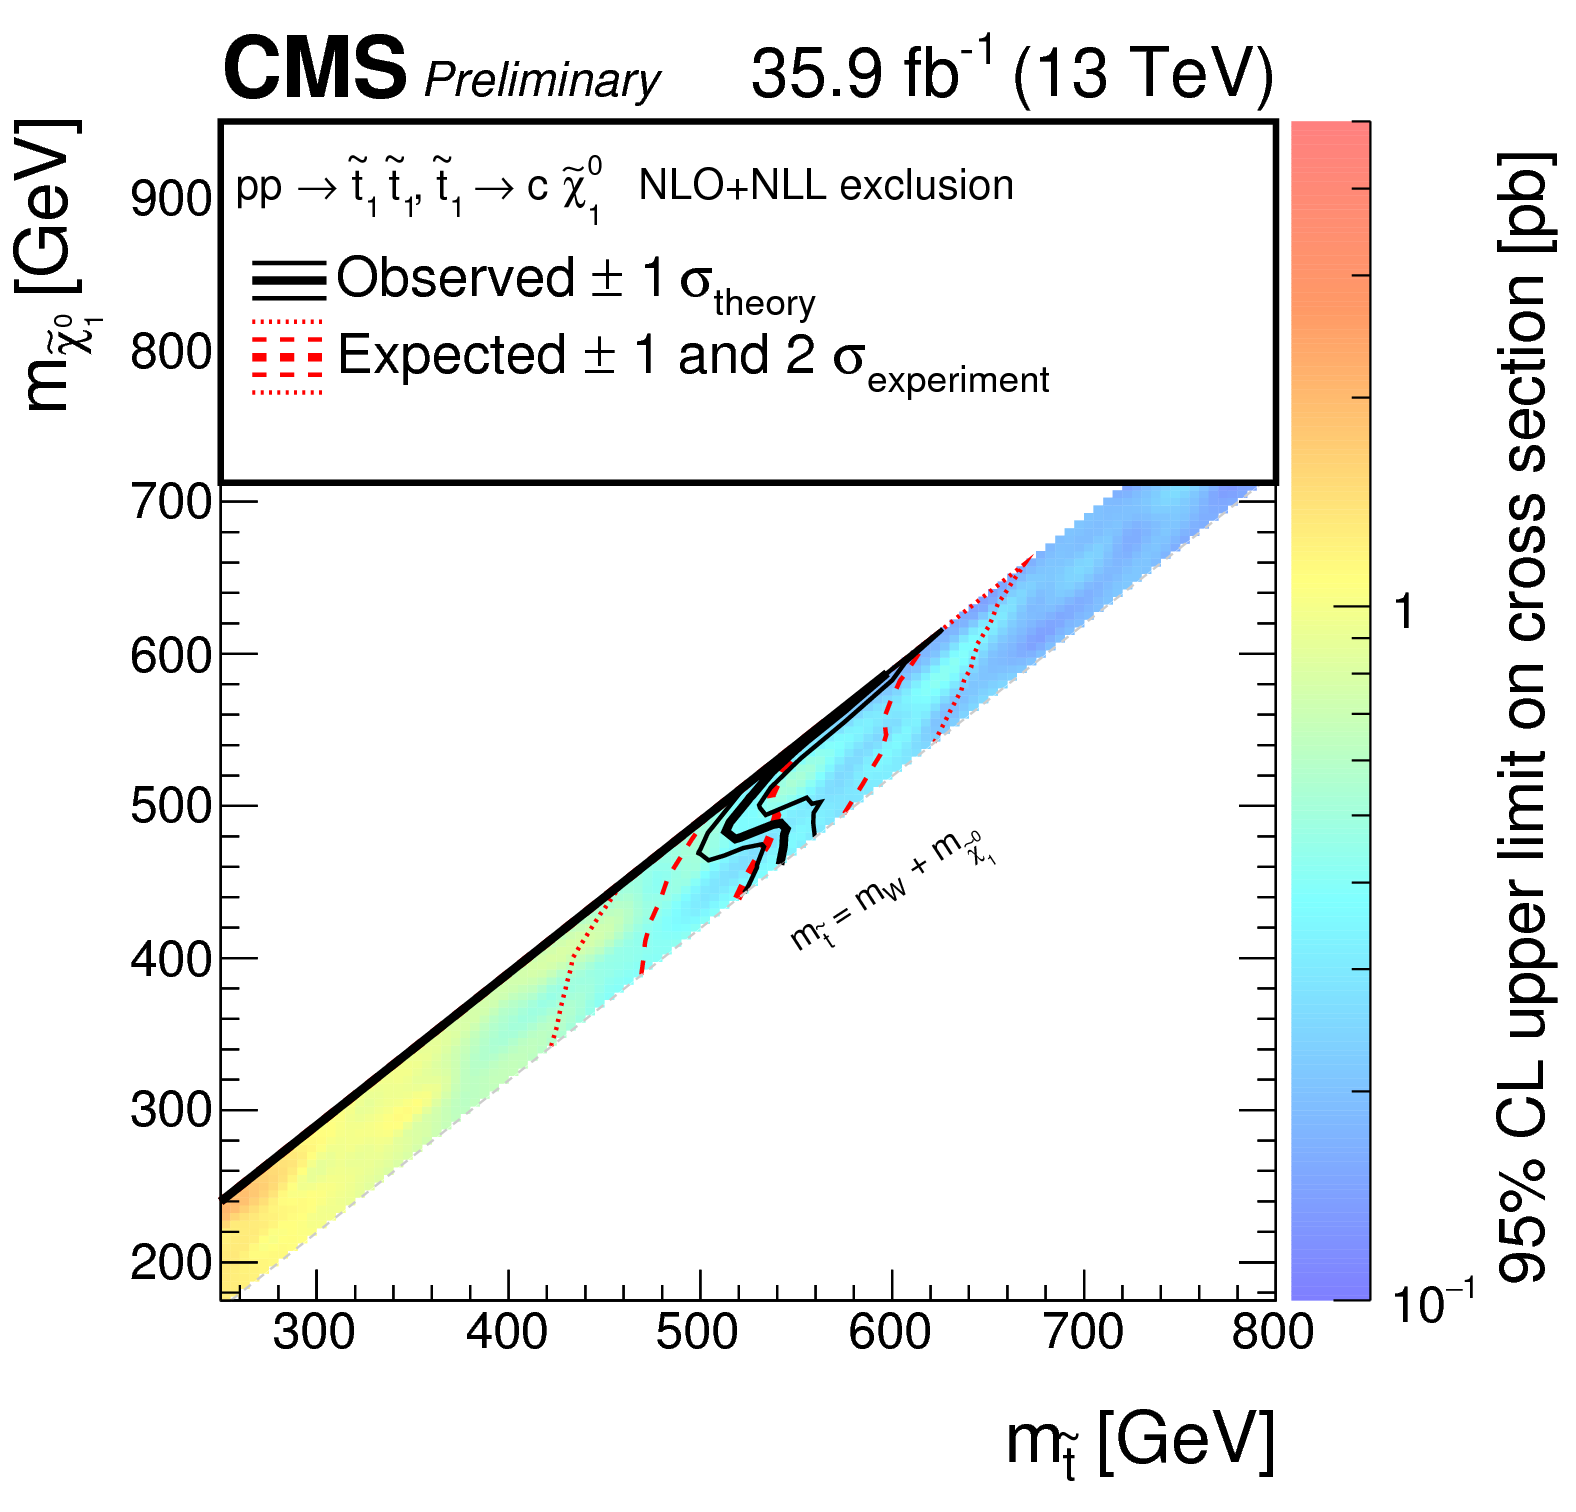
\includegraphics[width=0.6\textwidth]{figures/susyResults/T2ccXSEC}
            \label{fig:T2cc_excl}
        } \\
        \subfigure[T2cc: $\epsilon_{sig}$]{
            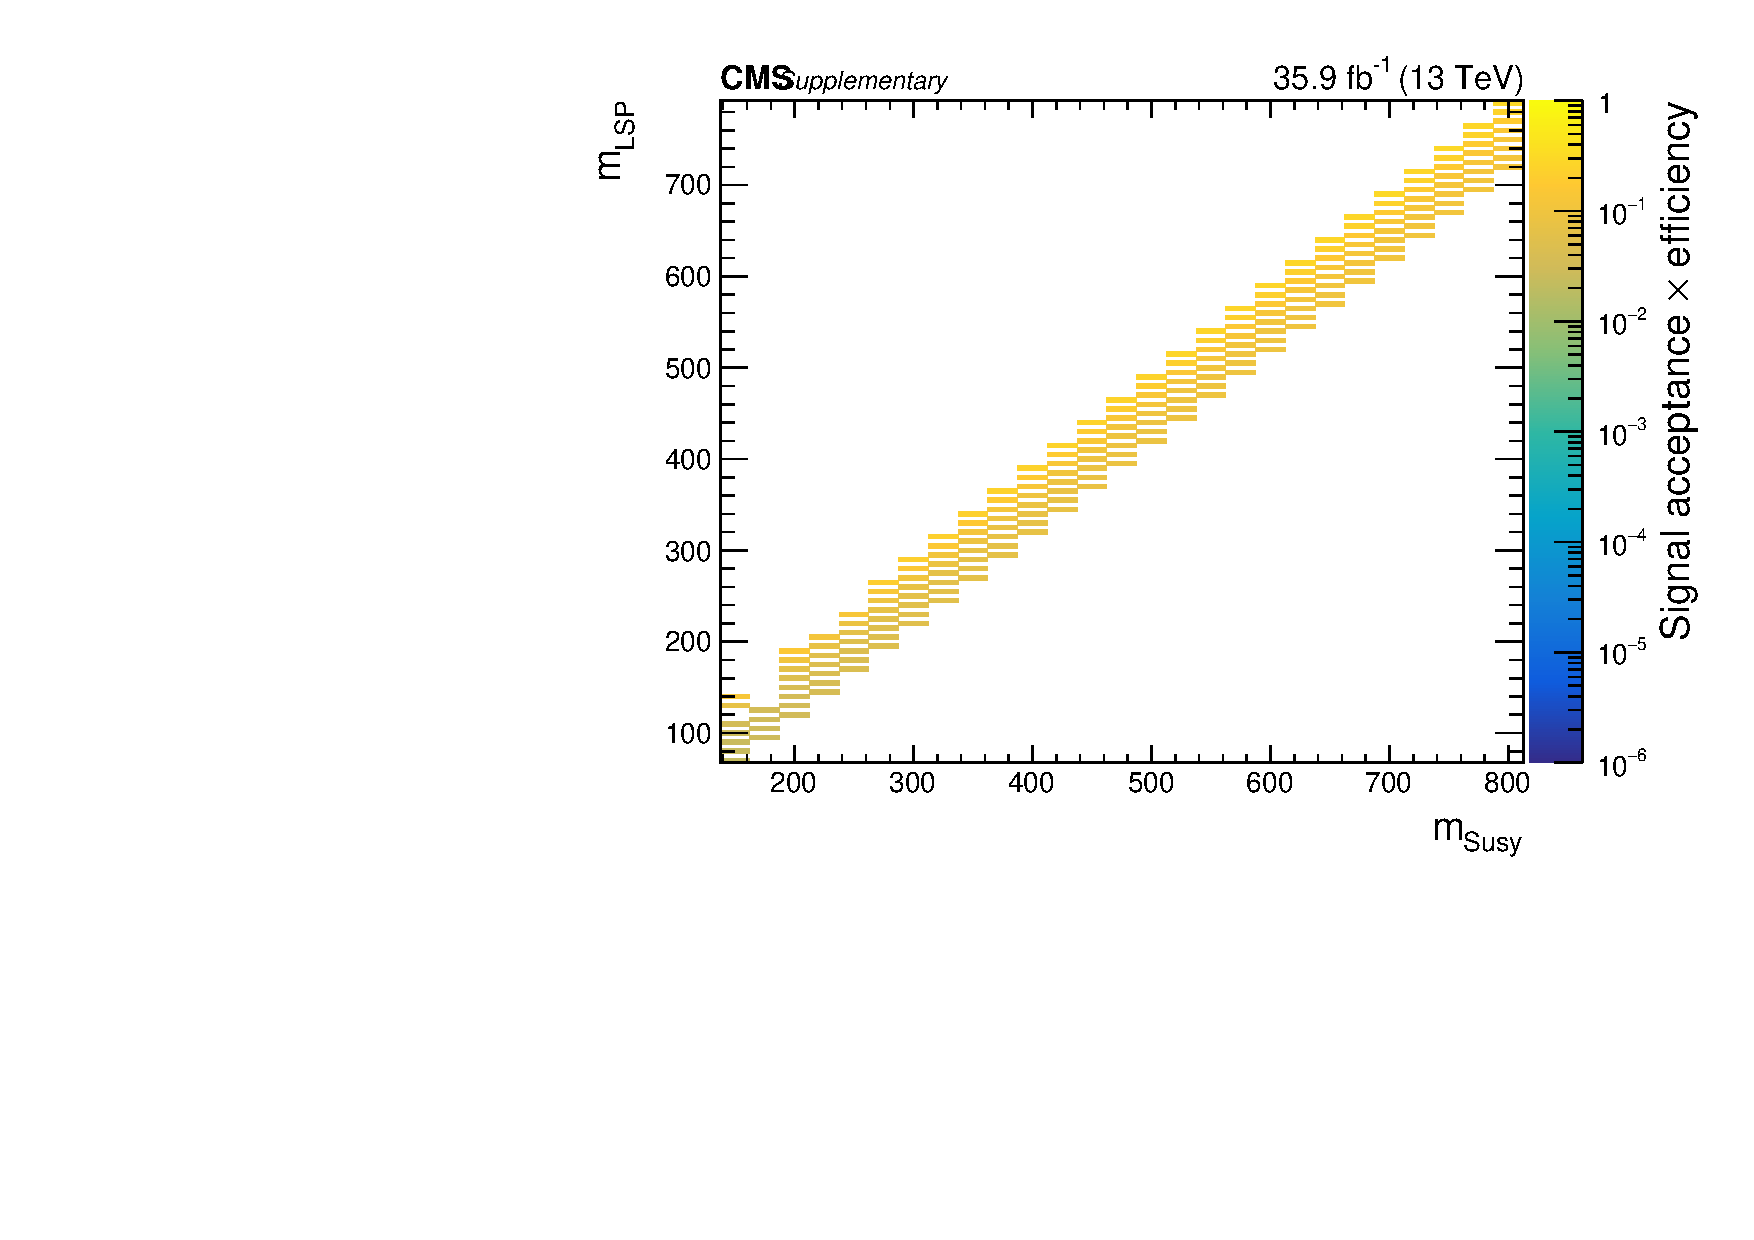
\includegraphics[width=0.45\textwidth]{figures/susyResults/T2cc_effs}
            \label{fig:T2cc_eff}
        } ~~
        \subfigure[T2cc: Most sensitive categories]{
            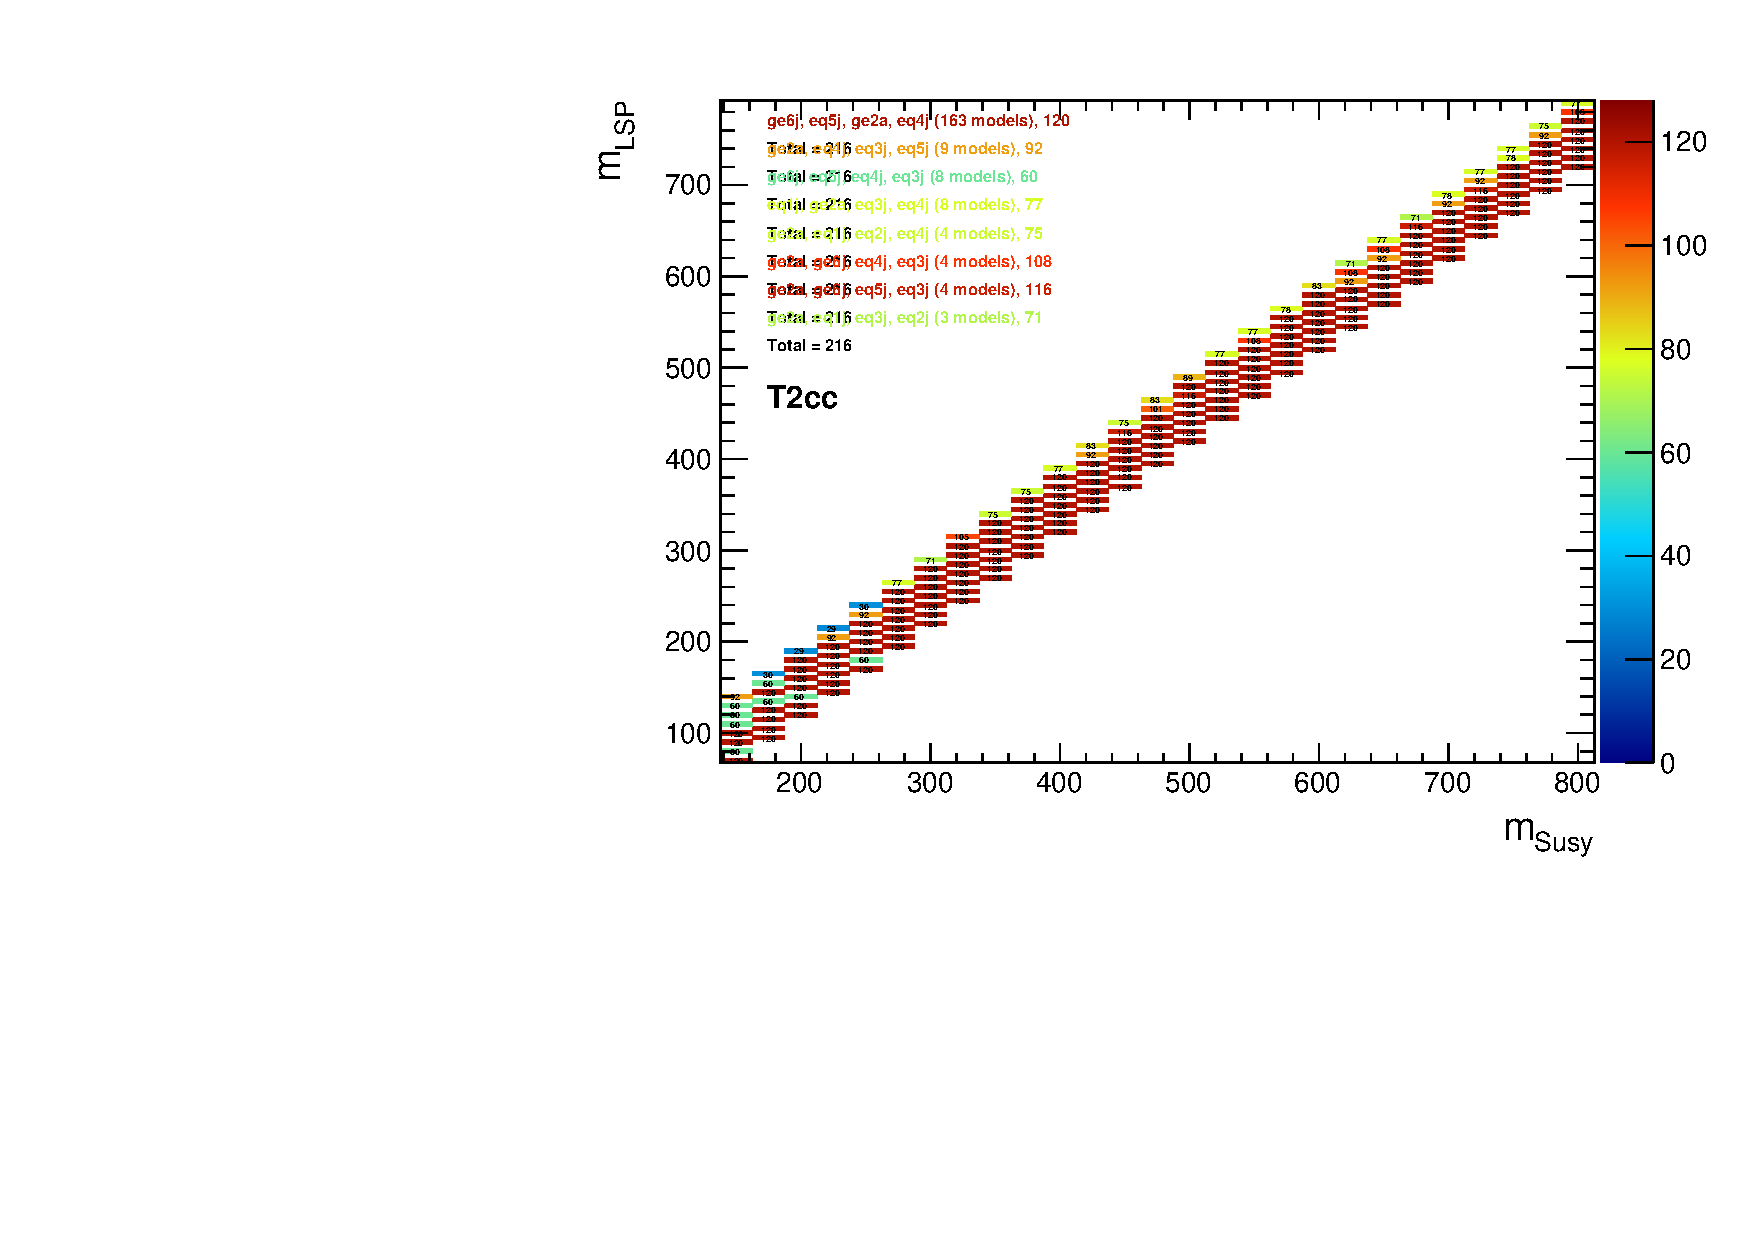
\includegraphics[width=0.45\textwidth]{figures/susyResults/T2cc_bitMap}
            \label{fig:T2cc_bitMap}
        } ~~
        \caption{Top: the 95\% C.L. observed upper limit on the cross section
            (histogram), with the expected (solid black line) observed
            (solid red line) exclusion contours. Bottom left: signal acceptance
            including all jet categories. Bottom right: bitmap representing the
            most sensitive jet categories for each mass point.}
        \label{fig:T2cc}
    \end{center}
\end{figure}

\newpage
\begin{figure}[h!]
    \begin{center}
        \subfigure[T2bb: Upper limit on the cross section in the mass plane]{
            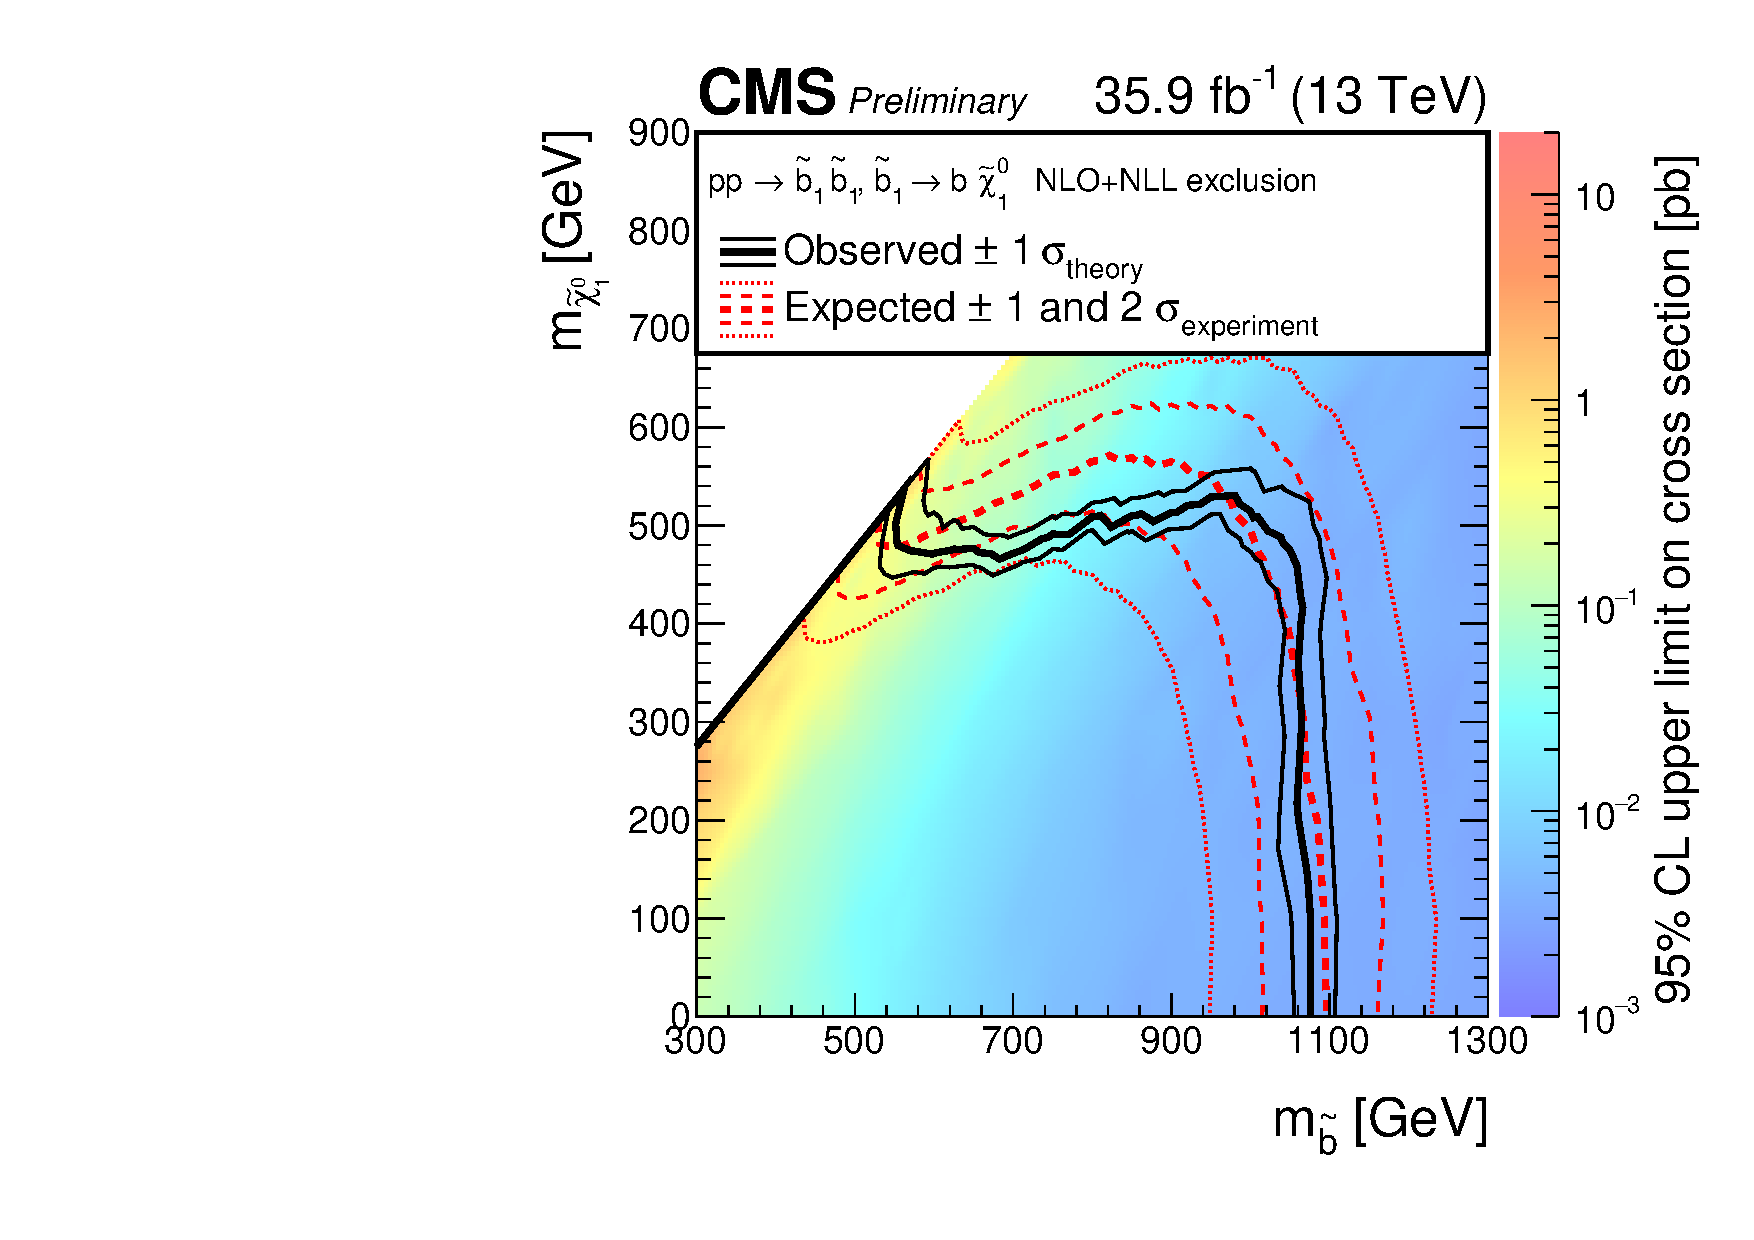
\includegraphics[width=0.6\textwidth]{figures/susyResults/T2bbXSEC}
            \label{fig:T2bb_excl}
        } \\
        \subfigure[T2bb: $\epsilon_{sig}$]{
            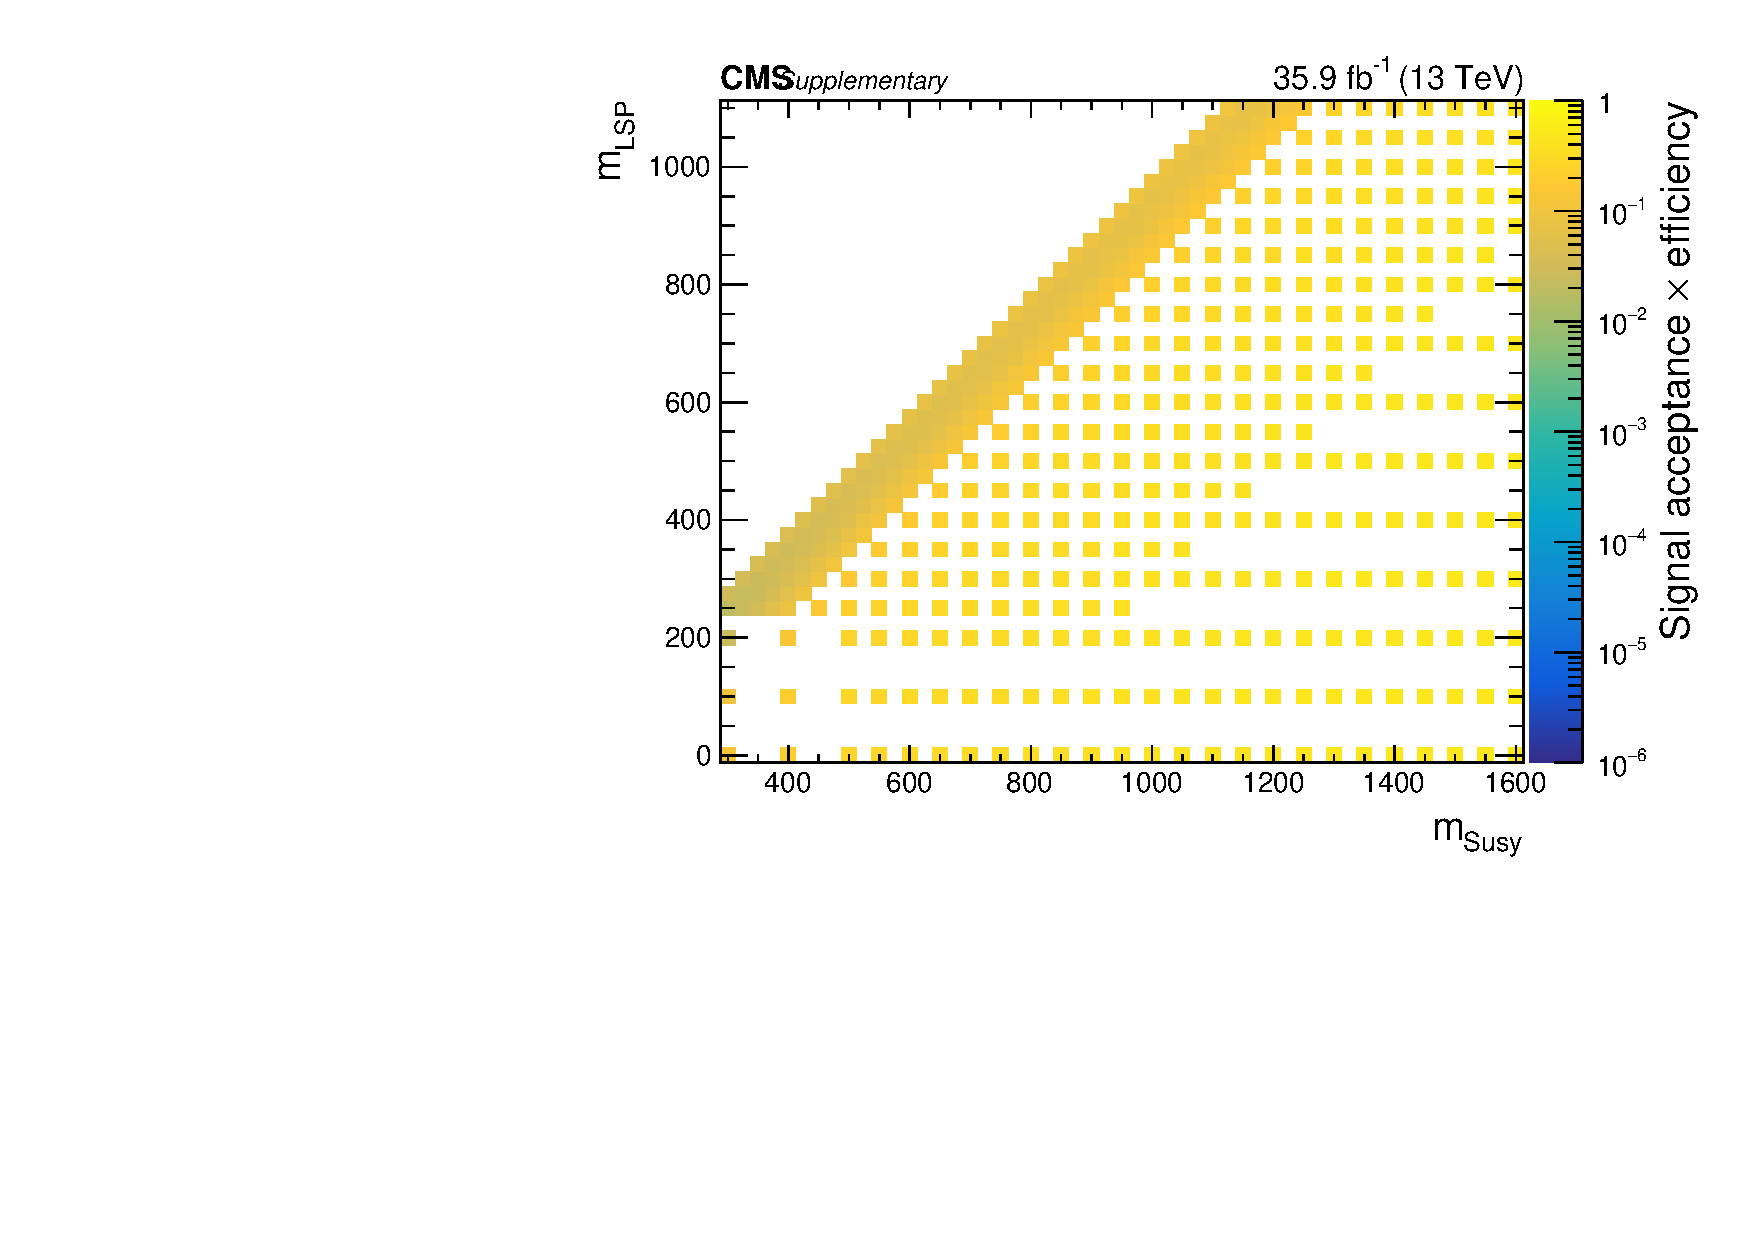
\includegraphics[width=0.45\textwidth]{figures/susyResults/T2bb_effs}
            \label{fig:T2bb_eff}
        } ~~
        \subfigure[T2bb: Most sensitive categories]{
            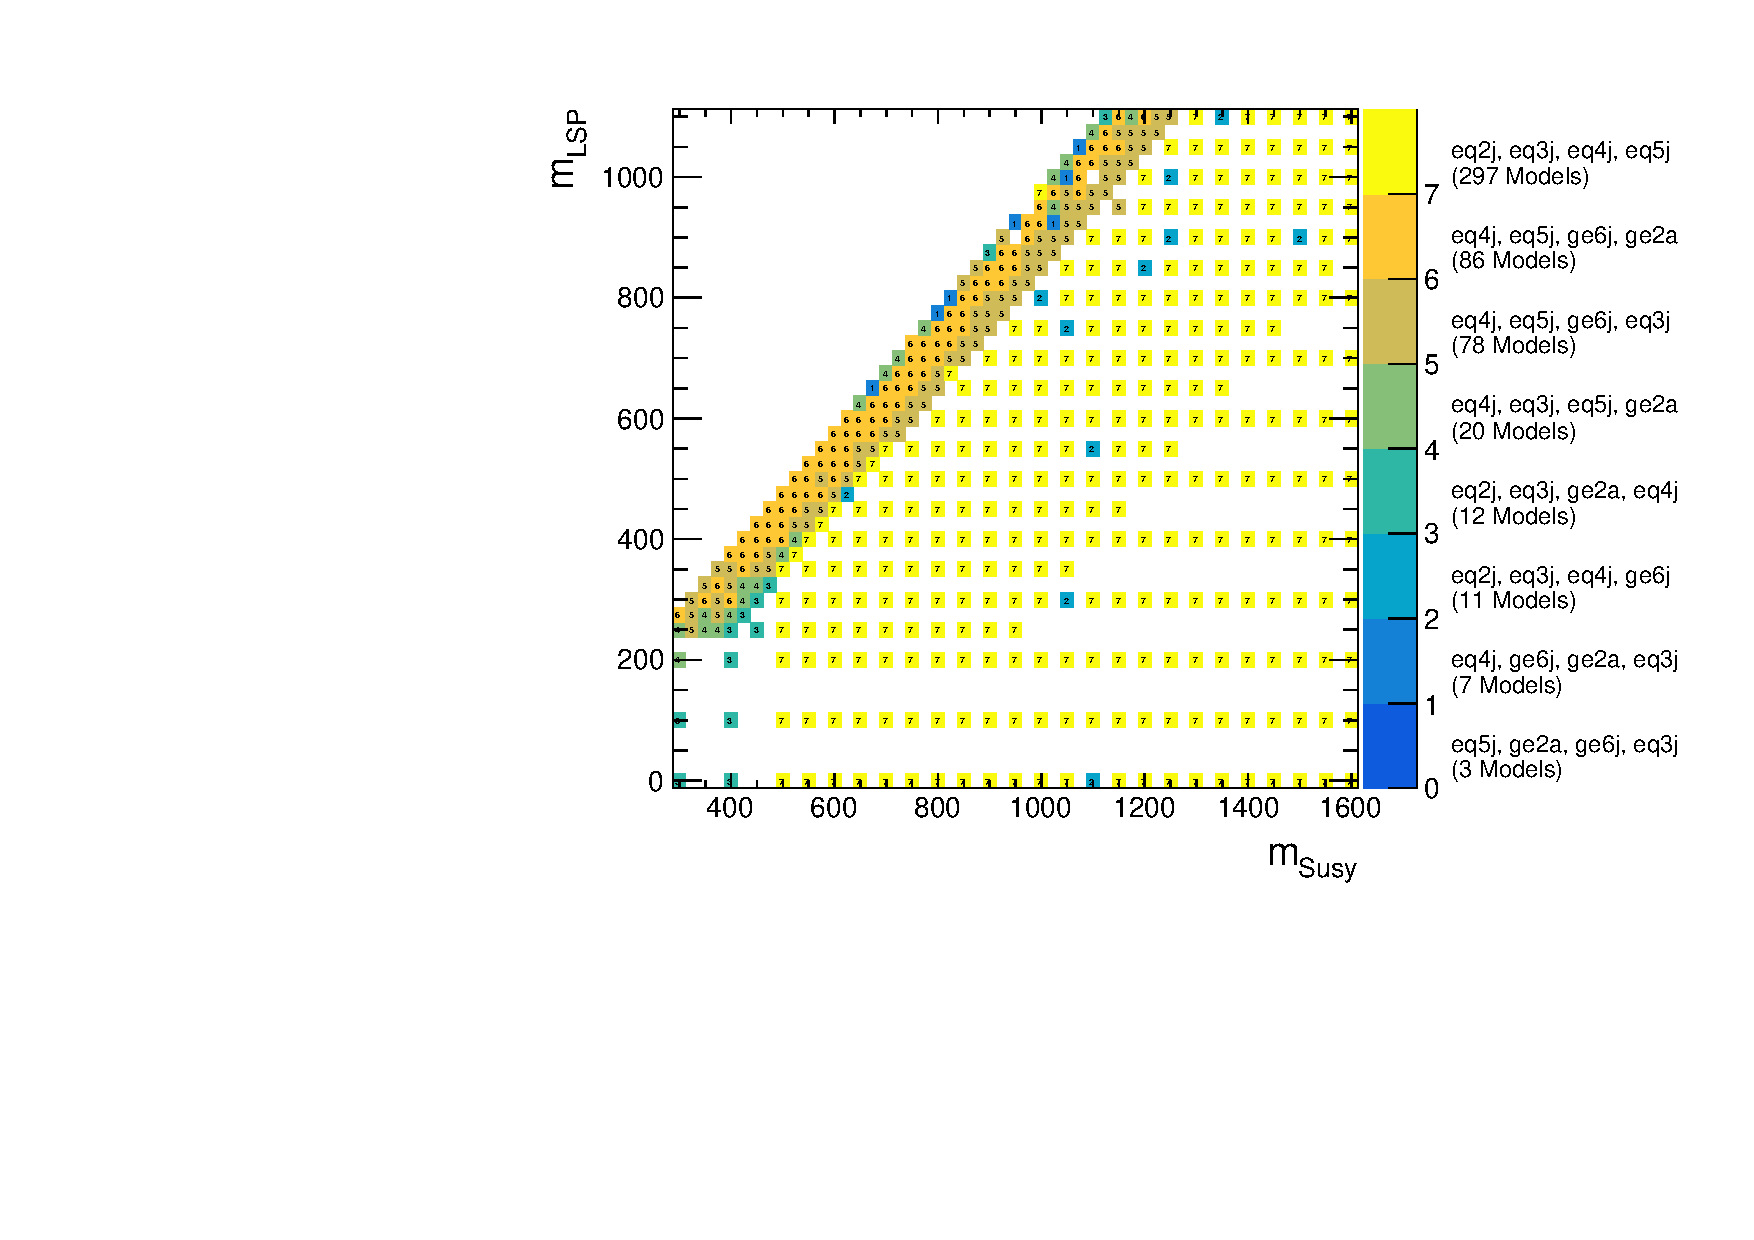
\includegraphics[width=0.45\textwidth]{figures/susyResults/T2bb_bitMap}
            \label{fig:T2bb_bitMap}
        } ~~
        \caption{Top: the 95\% C.L. observed upper limit on the cross section
            (histogram), with the expected (solid black line) observed
            (solid red line) exclusion contours. Bottom left: signal acceptance
            including all jet categories. Bottom right: bitmap representing the
            most sensitive jet categories for each mass point.}
        \label{fig:T2bb}
    \end{center}
\end{figure}

\newpage
\begin{figure}[h!]
    \begin{center}
        \subfigure[T2qq: Upper limit on the cross section in the mass plane]{
            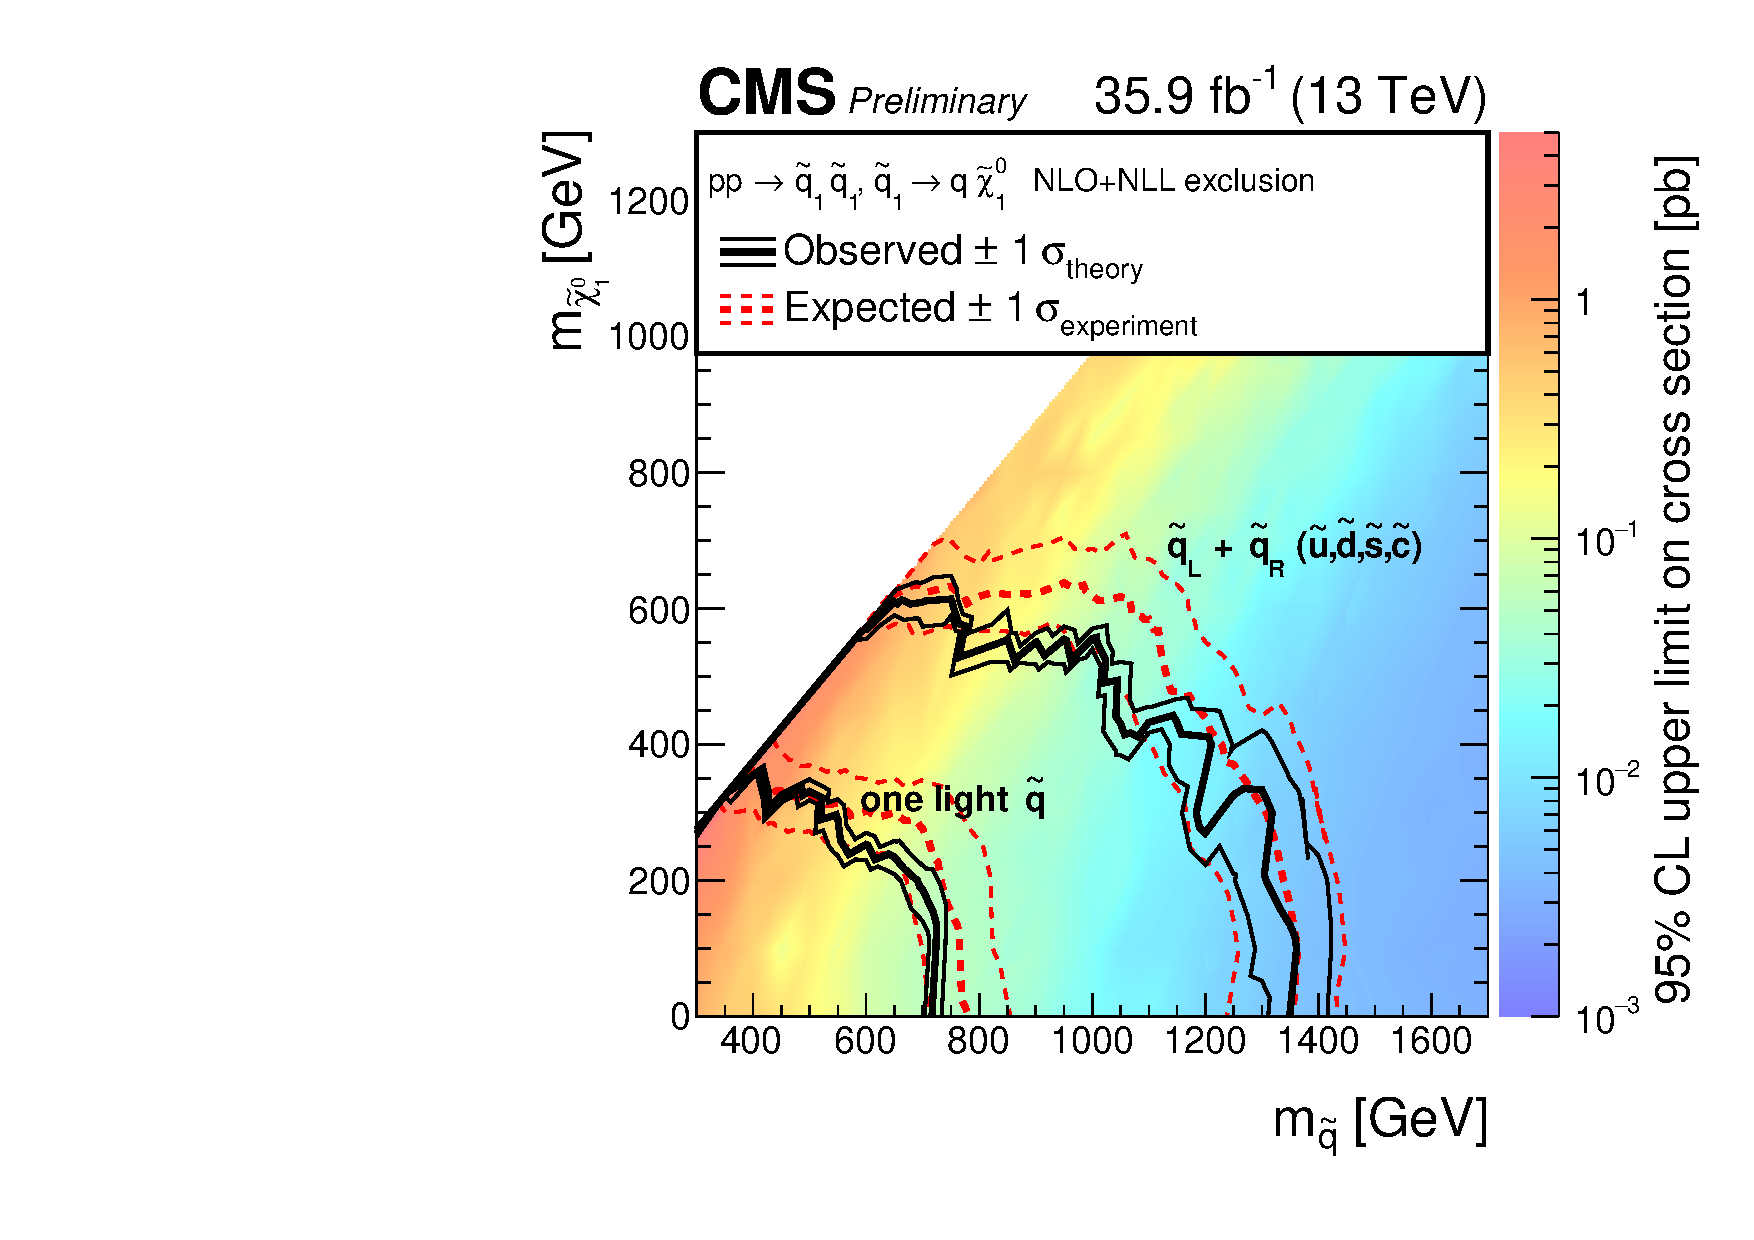
\includegraphics[width=0.6\textwidth]{figures/susyResults/T2qqXSEC}
            \label{fig:T2qq_excl}
        } \\
        \subfigure[T2qq: $\epsilon_{sig}$]{
            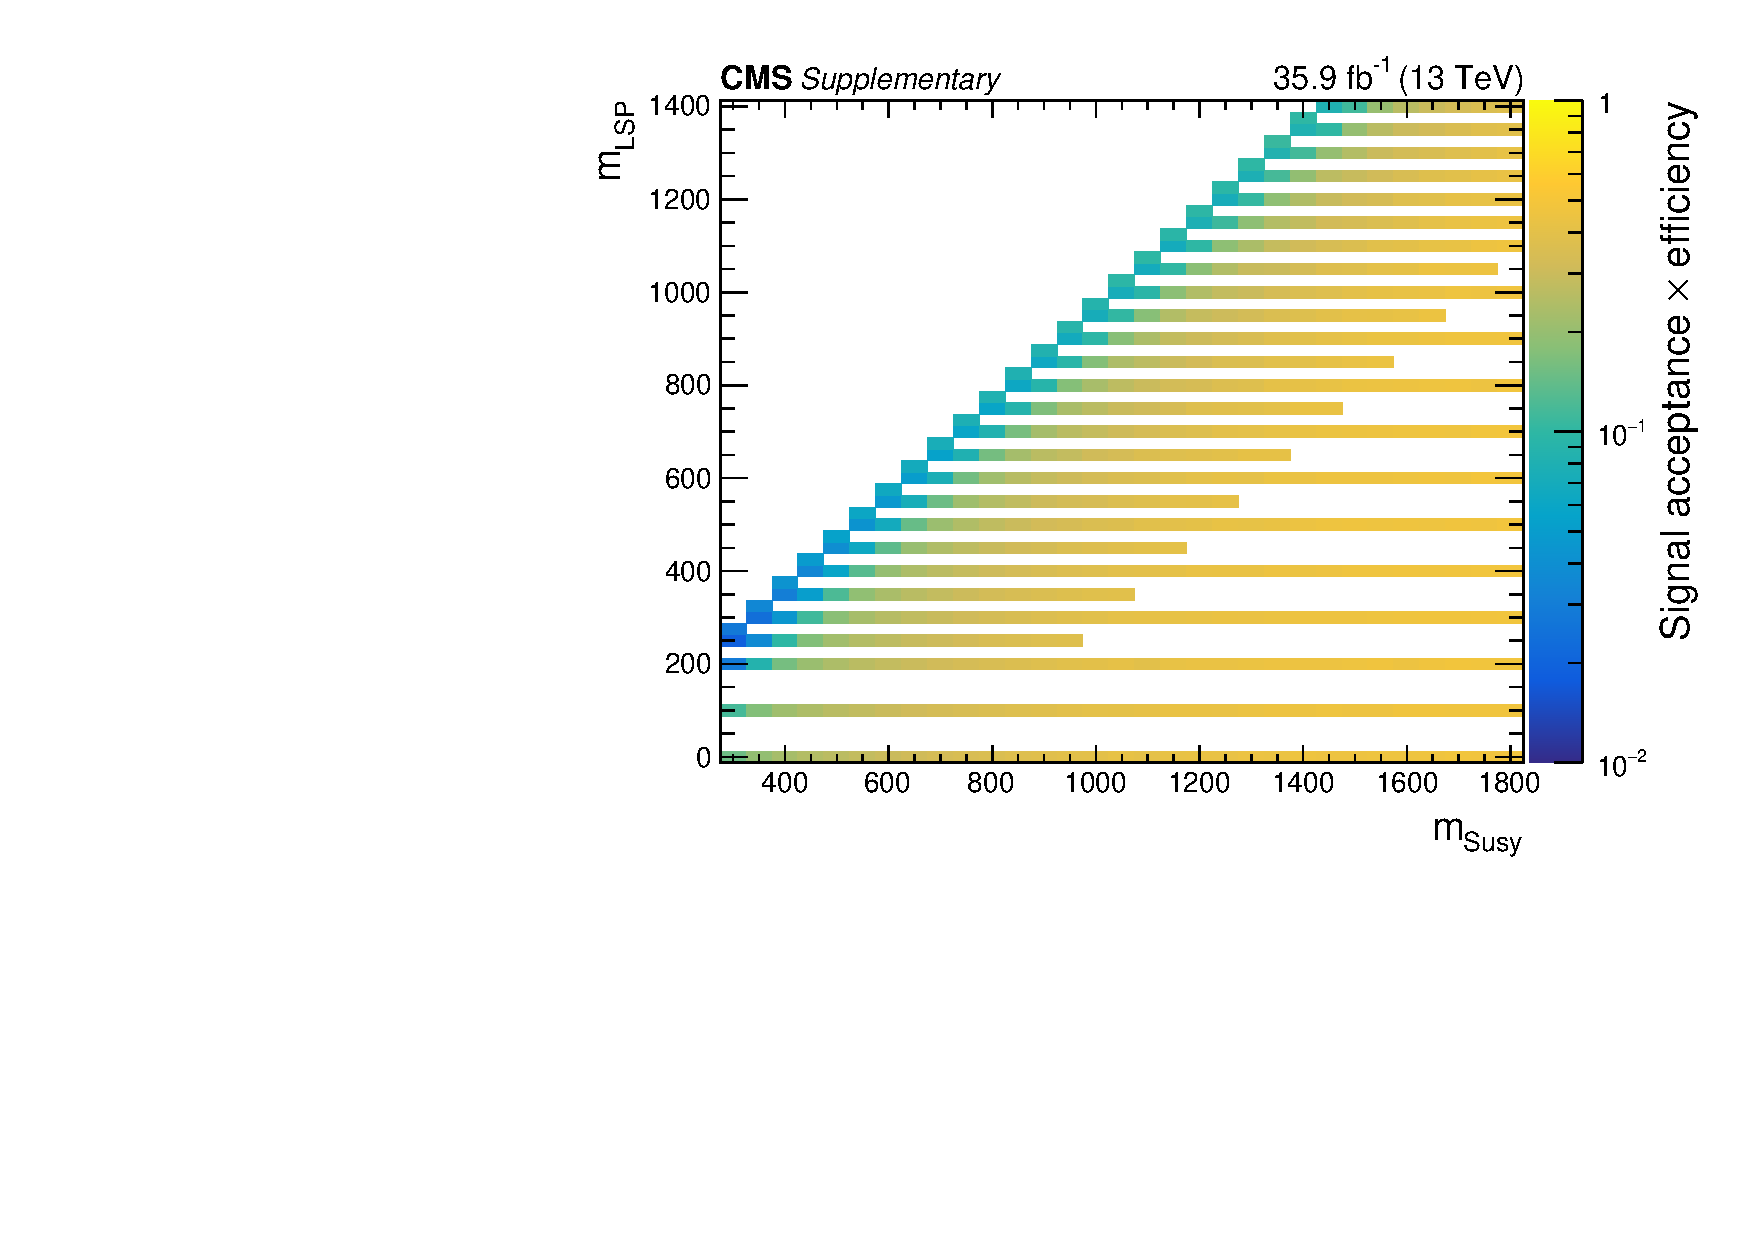
\includegraphics[width=0.45\textwidth]{figures/susyResults/T2qq_effs}
            \label{fig:T2qq_eff}
        } ~~
        \subfigure[T2qq: Most sensitive categories]{
            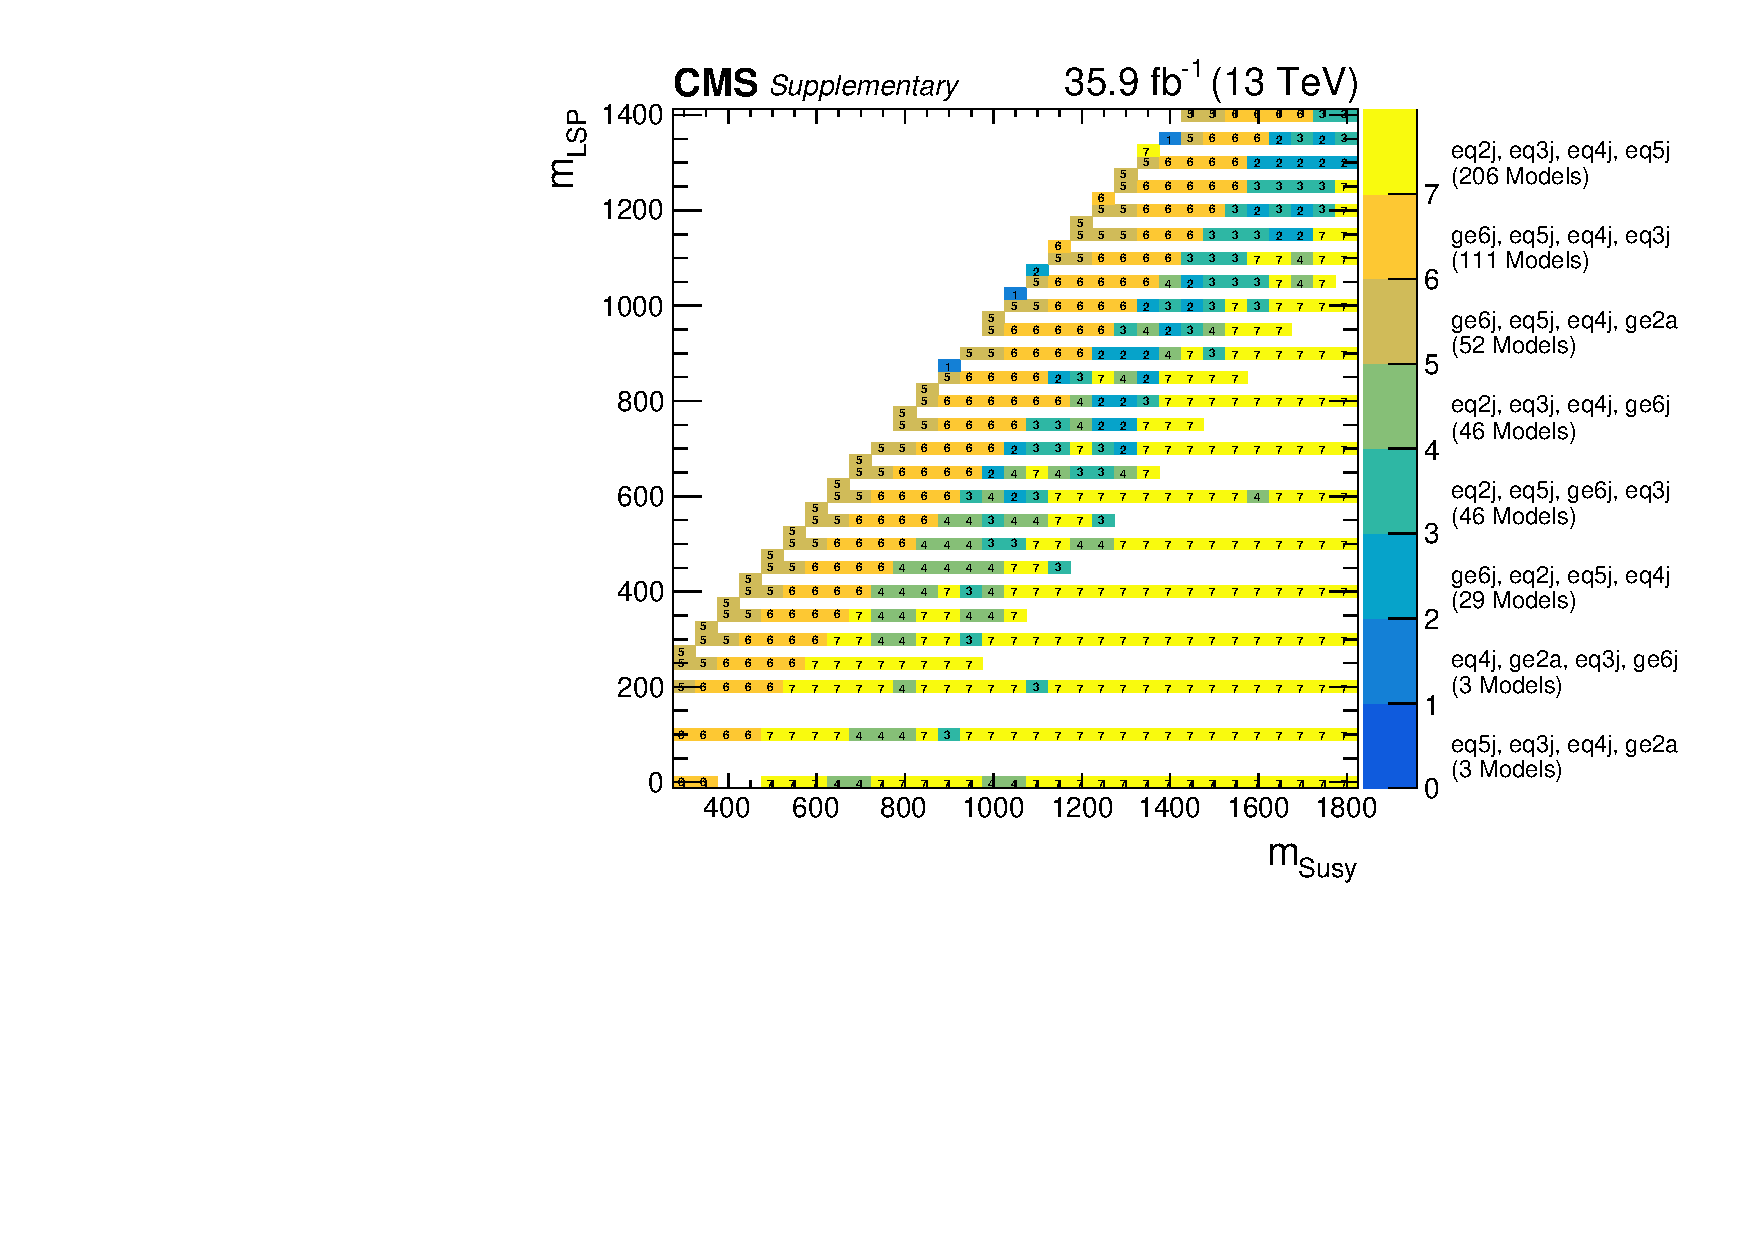
\includegraphics[width=0.45\textwidth]{figures/susyResults/T2qq_bitMap}
            \label{fig:T2qq_bitMap}
        } ~~
        \caption{Top: the 95\% C.L. observed upper limit on the cross section
            (histogram), with the expected (solid black line) observed
            (solid red line) exclusion contours. Bottom left: signal acceptance
            including all jet categories. Bottom right: bitmap representing the
            most sensitive jet categories for each mass point.}
        \label{fig:T2qq}
    \end{center}
\end{figure}


%\begin{figure*}[thp!]
%    \begin{center}
%        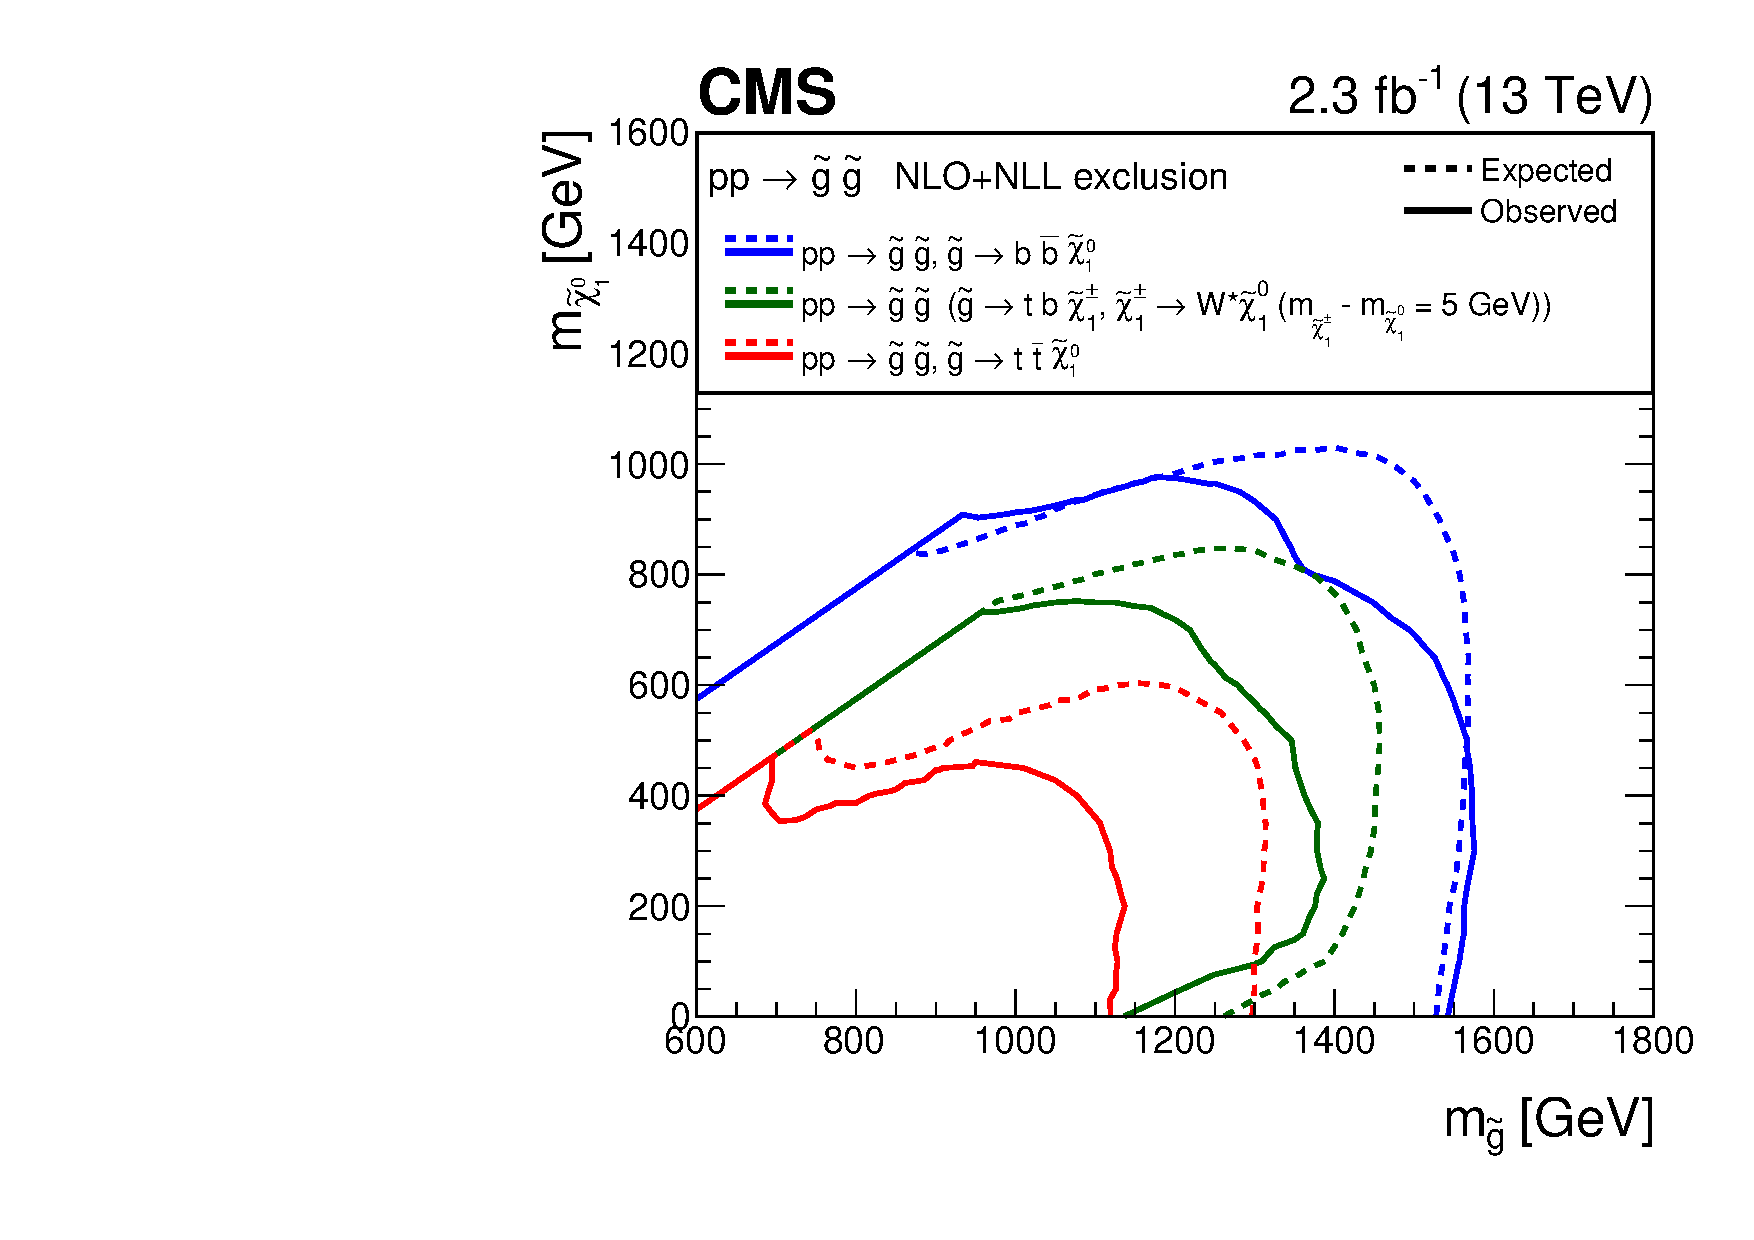
\includegraphics[width=0.49\textwidth]{figures/susyResults/gluinoSUMMARY.pdf} \\
%        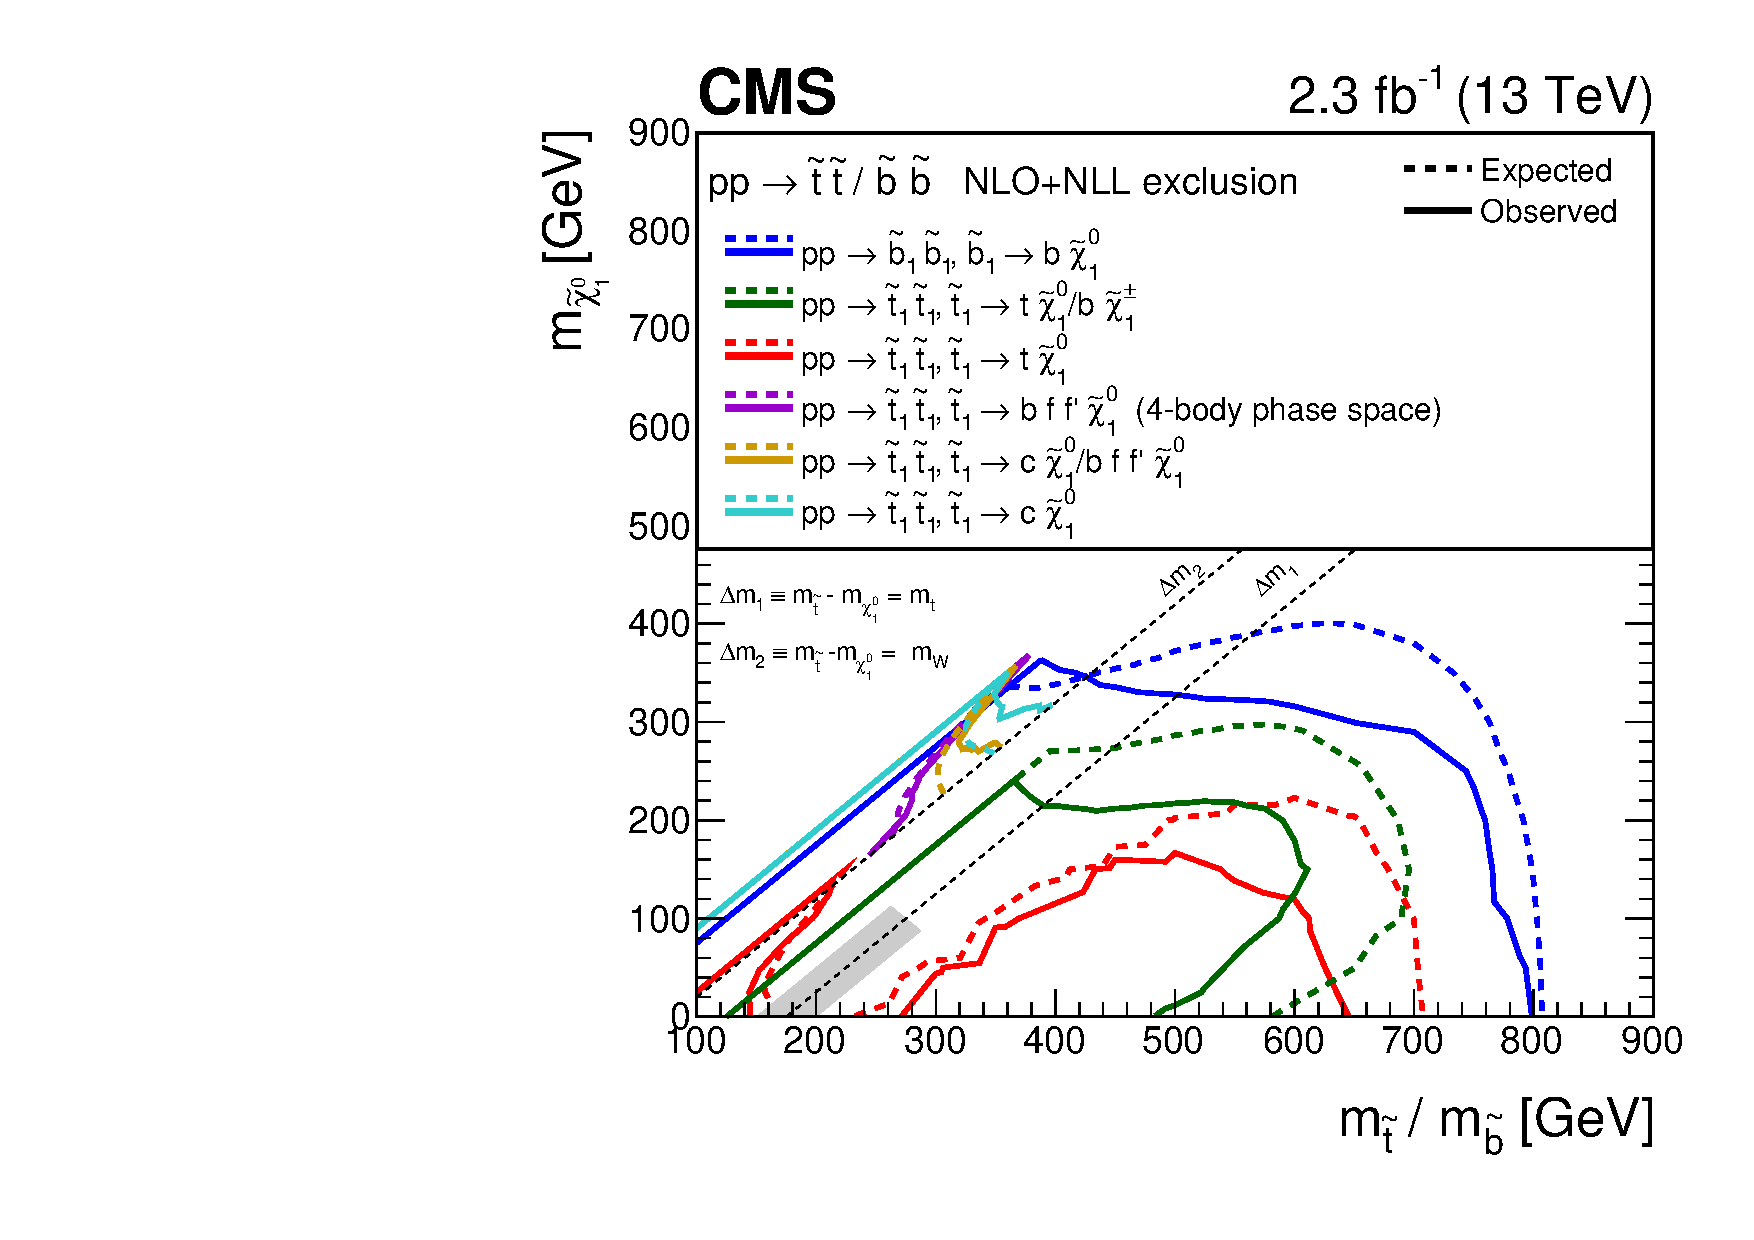
\includegraphics[width=0.49\textwidth]{figures/susyResults/allThirdGenSUMMARY.pdf} \\
%        \caption{Summary for the observed (solid lines) and expected
%            (dashed lines) exclusions in the $m_{\mathrm{Susy}},m_{\mathrm{LSP}}$
%            plane for the models considered in the analysis.Exclusion contours
%            are grouped into 4 summary plots according to the categorisation
%            presented at the begin of Sec.~\ref{sec:susy_results}:
%            ``Gluino-mediated production of off-shell (decoupled) 3rd generation
%                squarks'' (top right),
%            ``Direct production of 3rd generation squarks'' (bottom right).
%        \label{fig:summary-excl-plots} }
%    \end{center}
%\end{figure*}

\newpage
Gluino masses up to $\sim$2050 GeV are excluded (T1bbbb). Stop production is
excluded up to $\sim$1050 GeV in the 2-body decay to top quarks (T2tt), and up
to $\sim$550 GeV in the compressed region, in the decay to charm quarks (T2cc).
Sbottom (squark) masses smaller than $\sim$1100 GeV are excluded for small LSP
masses (T2bb,T2qq). For the models considered, the exclusion exceeds the one of
the 13 TeV ICHEP data.

%%____________________________________________________________________________||
